\section{Usage Characteristics}
\label{sec:character}


\subsection{Experiment Distributions} 
\begin{figure}[htbp] \begin{center}
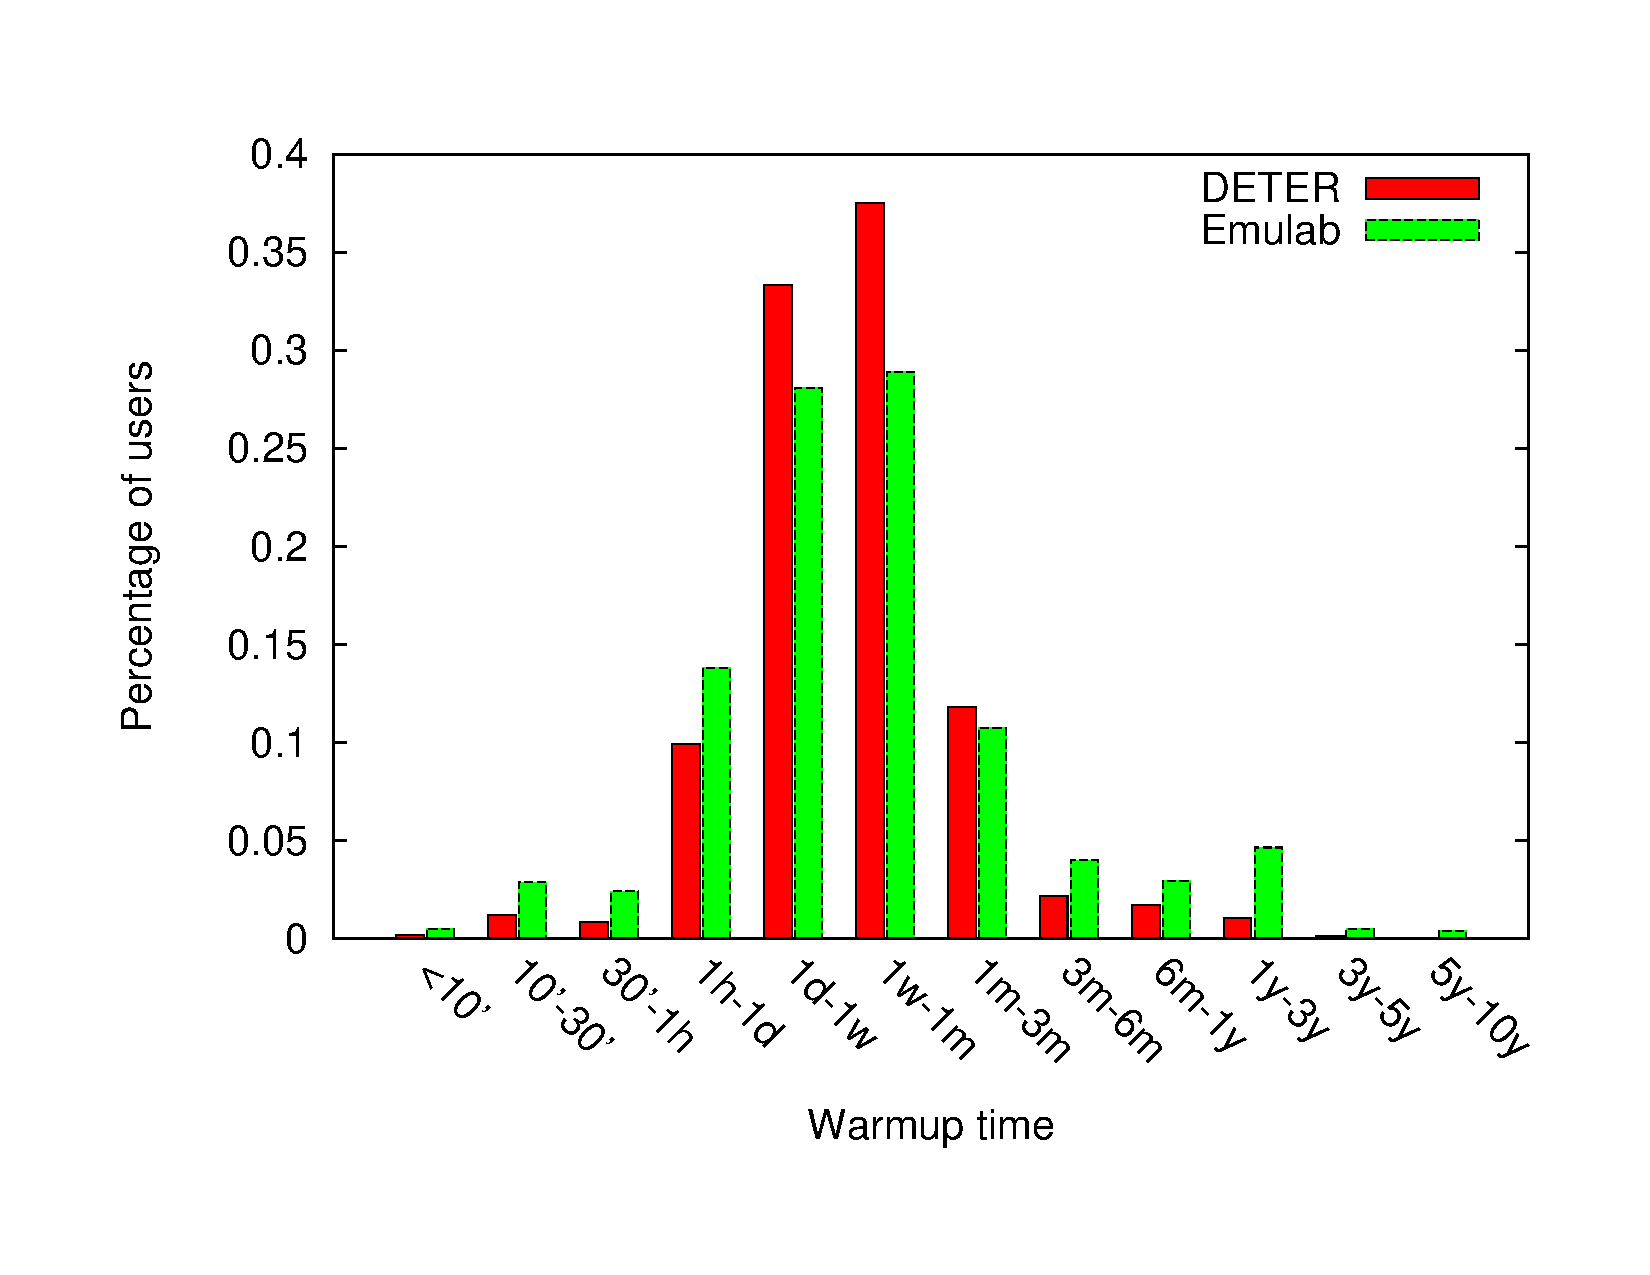
\includegraphics[width=3in]{figs/warmup_user.pdf} 
\caption{User warmup time in DETER and Emulab} 
\label{warmupus} \end{center} \end{figure}

\begin{figure}[htbp] \begin{center}
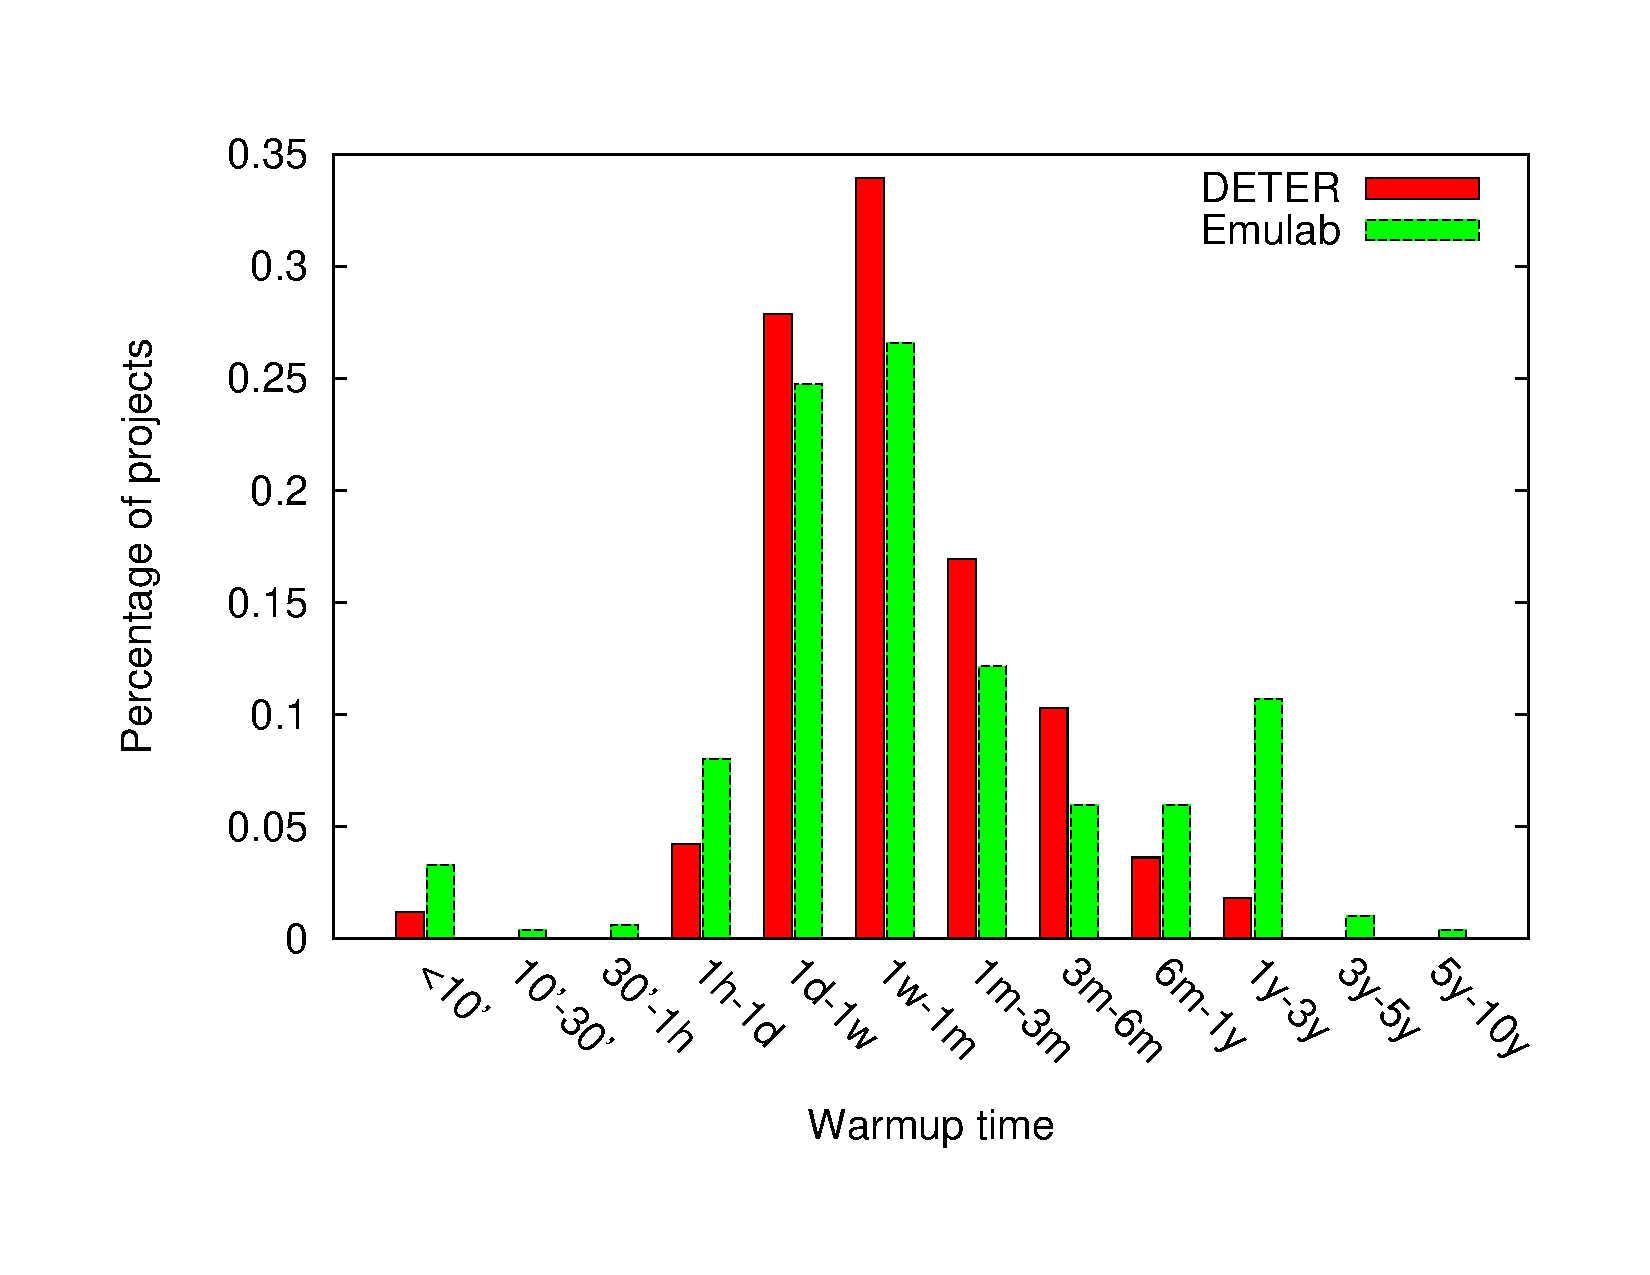
\includegraphics[width=3in]{figs/warmup_proj.pdf} 
\caption{Project warmup time in DETER and Emulab} \label{warmuppr} \end{center}
\end{figure}


\begin{figure}[htbp] \begin{center}
\includegraphics[width=3in]{figs/warmup_inact_user.pdf} 
\caption{User warmup and inactive time} \label{warmupinus} \end{center} \end{figure}


\begin{figure}[htbp] \begin{center}
\includegraphics[width=3in]{figs/warmup_inact_proj.pdf} \caption{Project
warmup and inactive time} \label{warmupinpr} \end{center} \end{figure}

If we use the maximum value of the warmup time for the threshold then
the starred rows in the table \ref{cleaning} apply.

We now look at number of projects per research category. This is shown
in table \ref{projrc}. We took DDoS, worm and botnet out of attack
category because they are popular topics in recent years.

\begin{table}[htdp] \begin{center} \begin{tabular}{|c|c|} \hline
Research category & Projects \\\hline Attacks & 48  \\ DDoS & 18 \\
Architecture & 14\\ Infrastructure & 12 \\ Testbeds & 12 \\ Worms & 11
\\ Evaluation & 8 \\ Privacy & 6 \\ Botnets & 4 \\ \hline \end{tabular}
\end{center} \caption{Projects per research category} \label{projrc}
\end{table}%



Say exps from outcome projects follow same trends as all so we don't
show them here.

\begin{figure}[htbp] \begin{center}
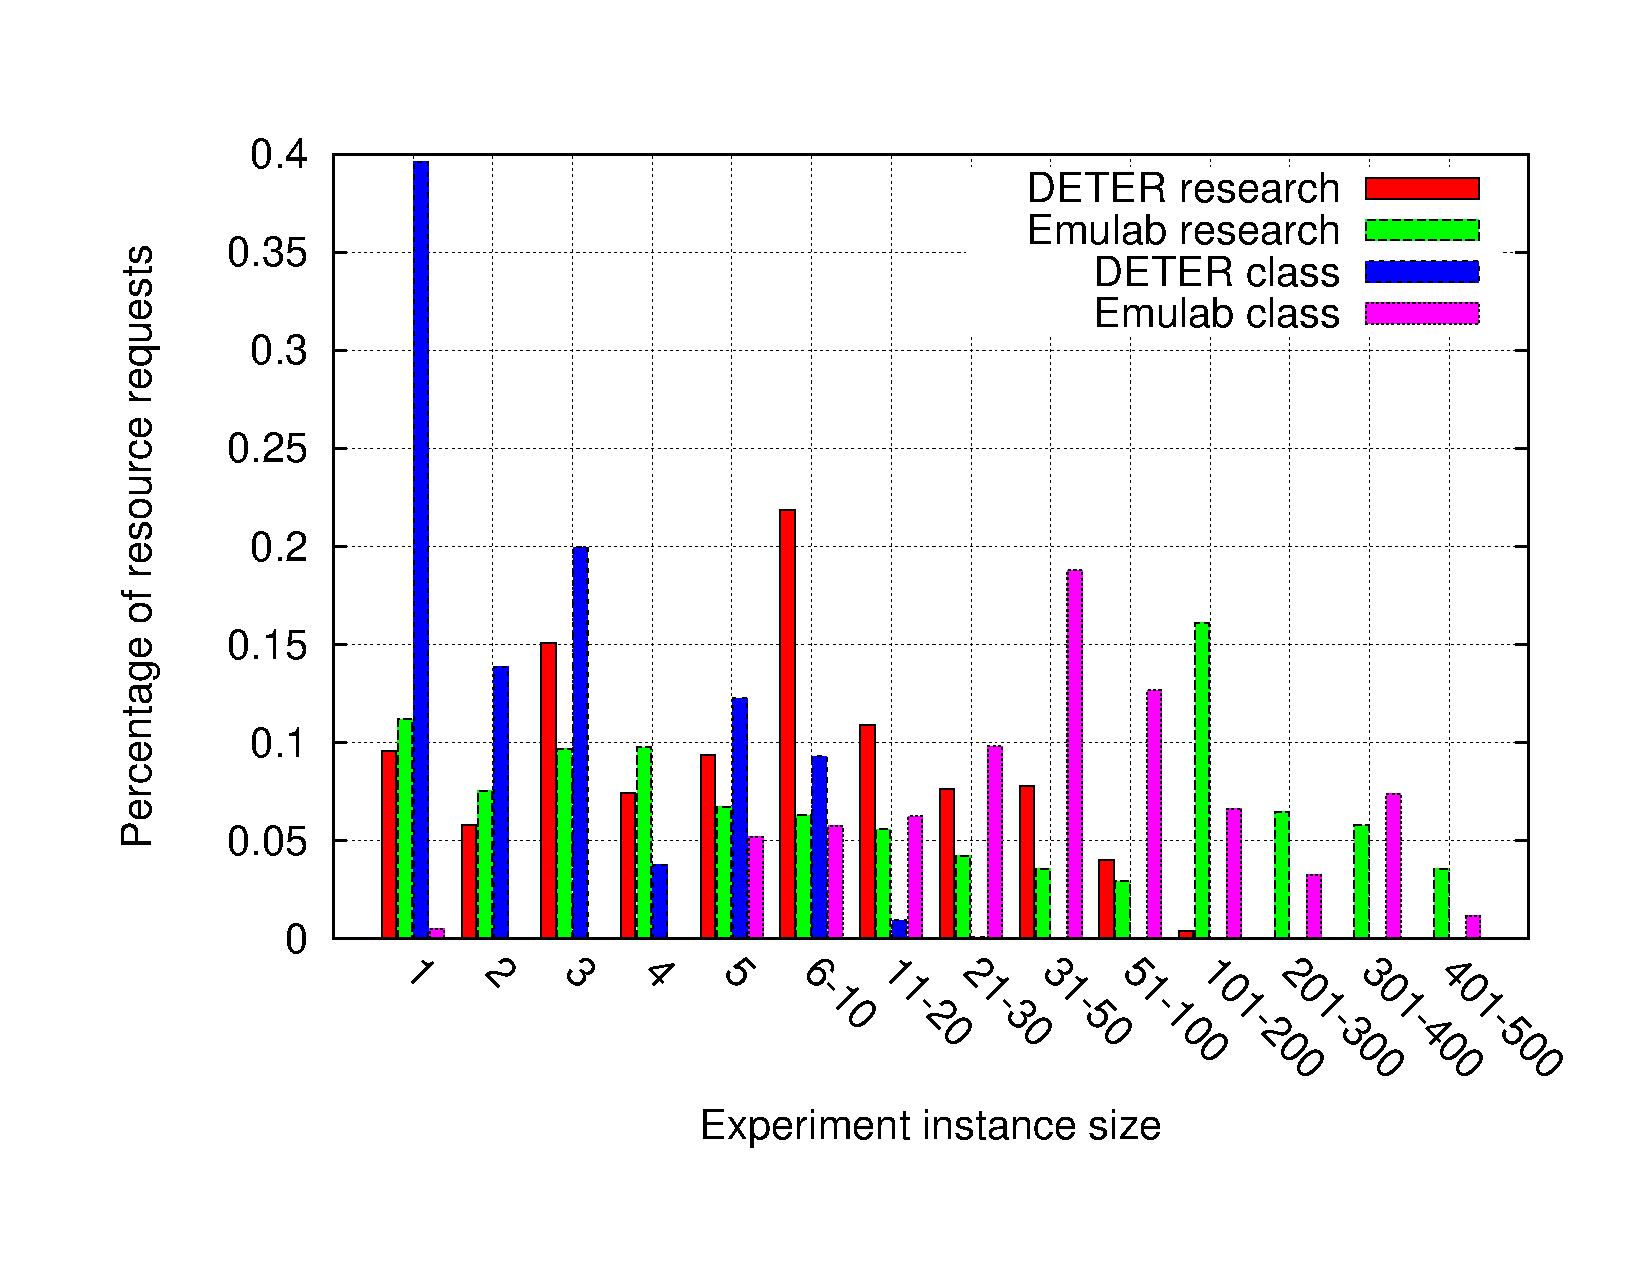
\includegraphics[width=3in,type=pdf,ext=.pdf,read=.pdf]
{figs/exp.size.gnu} \caption{Experiment instance size} \label{expsize} \end{center}
\end{figure}

\begin{figure}[htbp] \begin{center}
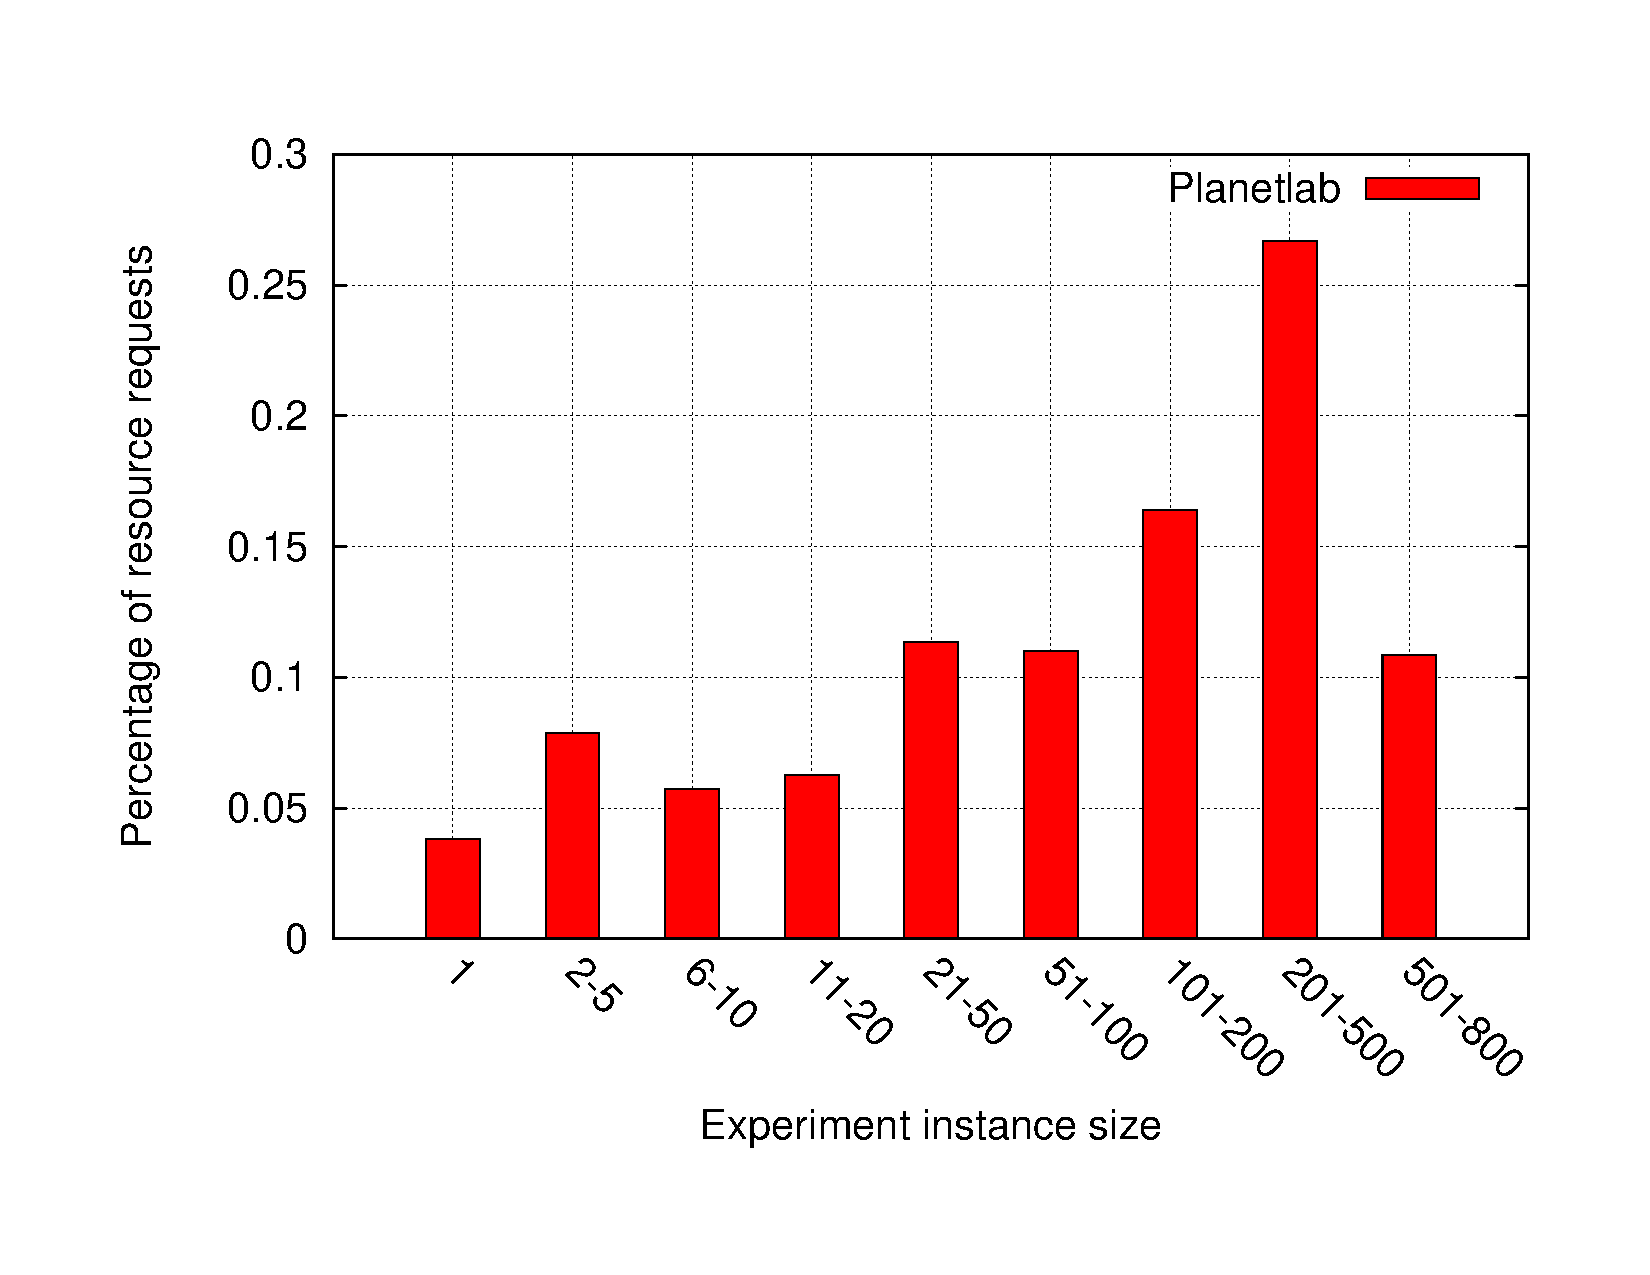
\includegraphics[width=3in,type=pdf,ext=.pdf,read=.pdf]
{figs/planet.size.gnu} \caption{Experiment instance size in Planetlab} \label{expsize}
\end{center} \end{figure}

\begin{figure}[htbp] \begin{center} 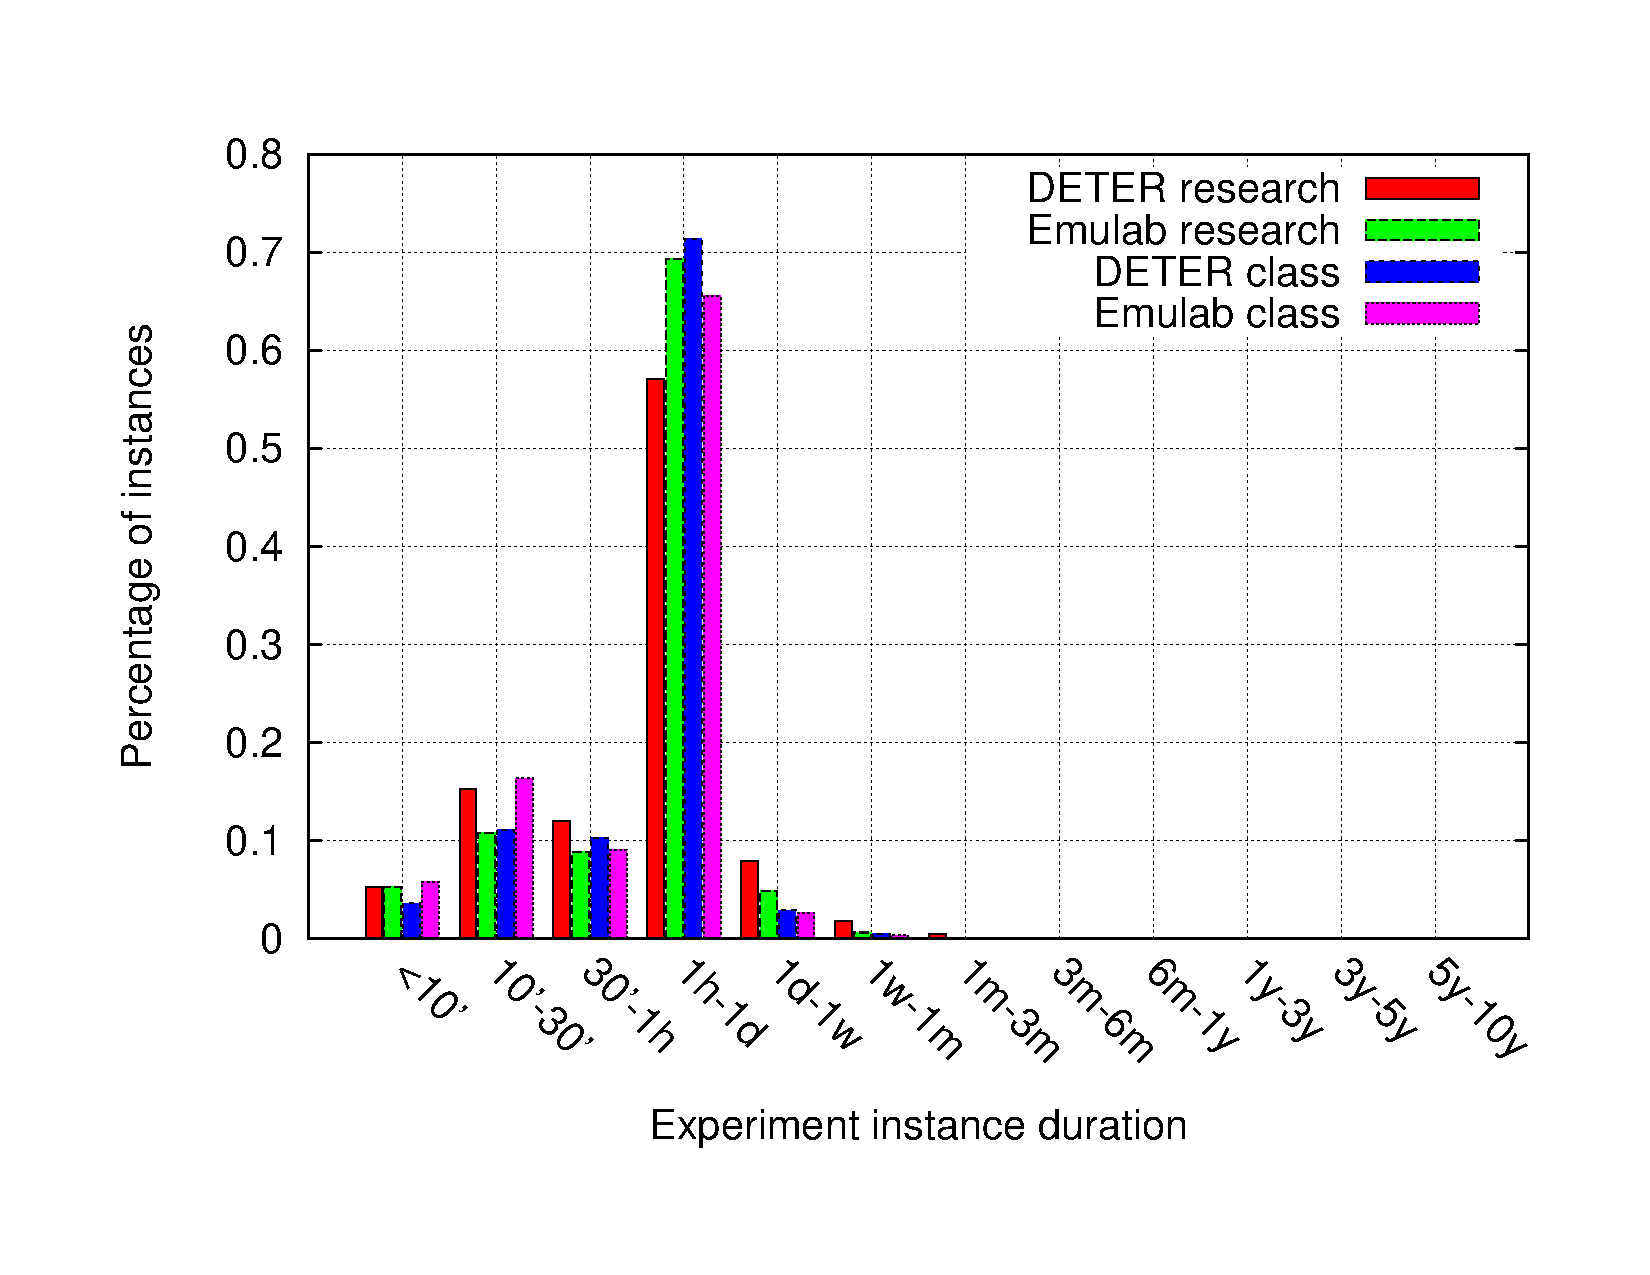
\includegraphics[width=3in,
type=pdf,ext=.pdf,read=.pdf]{figs/exp.dur.gnu} \caption{Experiment
instance duration} \label{expdur} \end{center} \end{figure}

\begin{figure}[htbp] \begin{center} 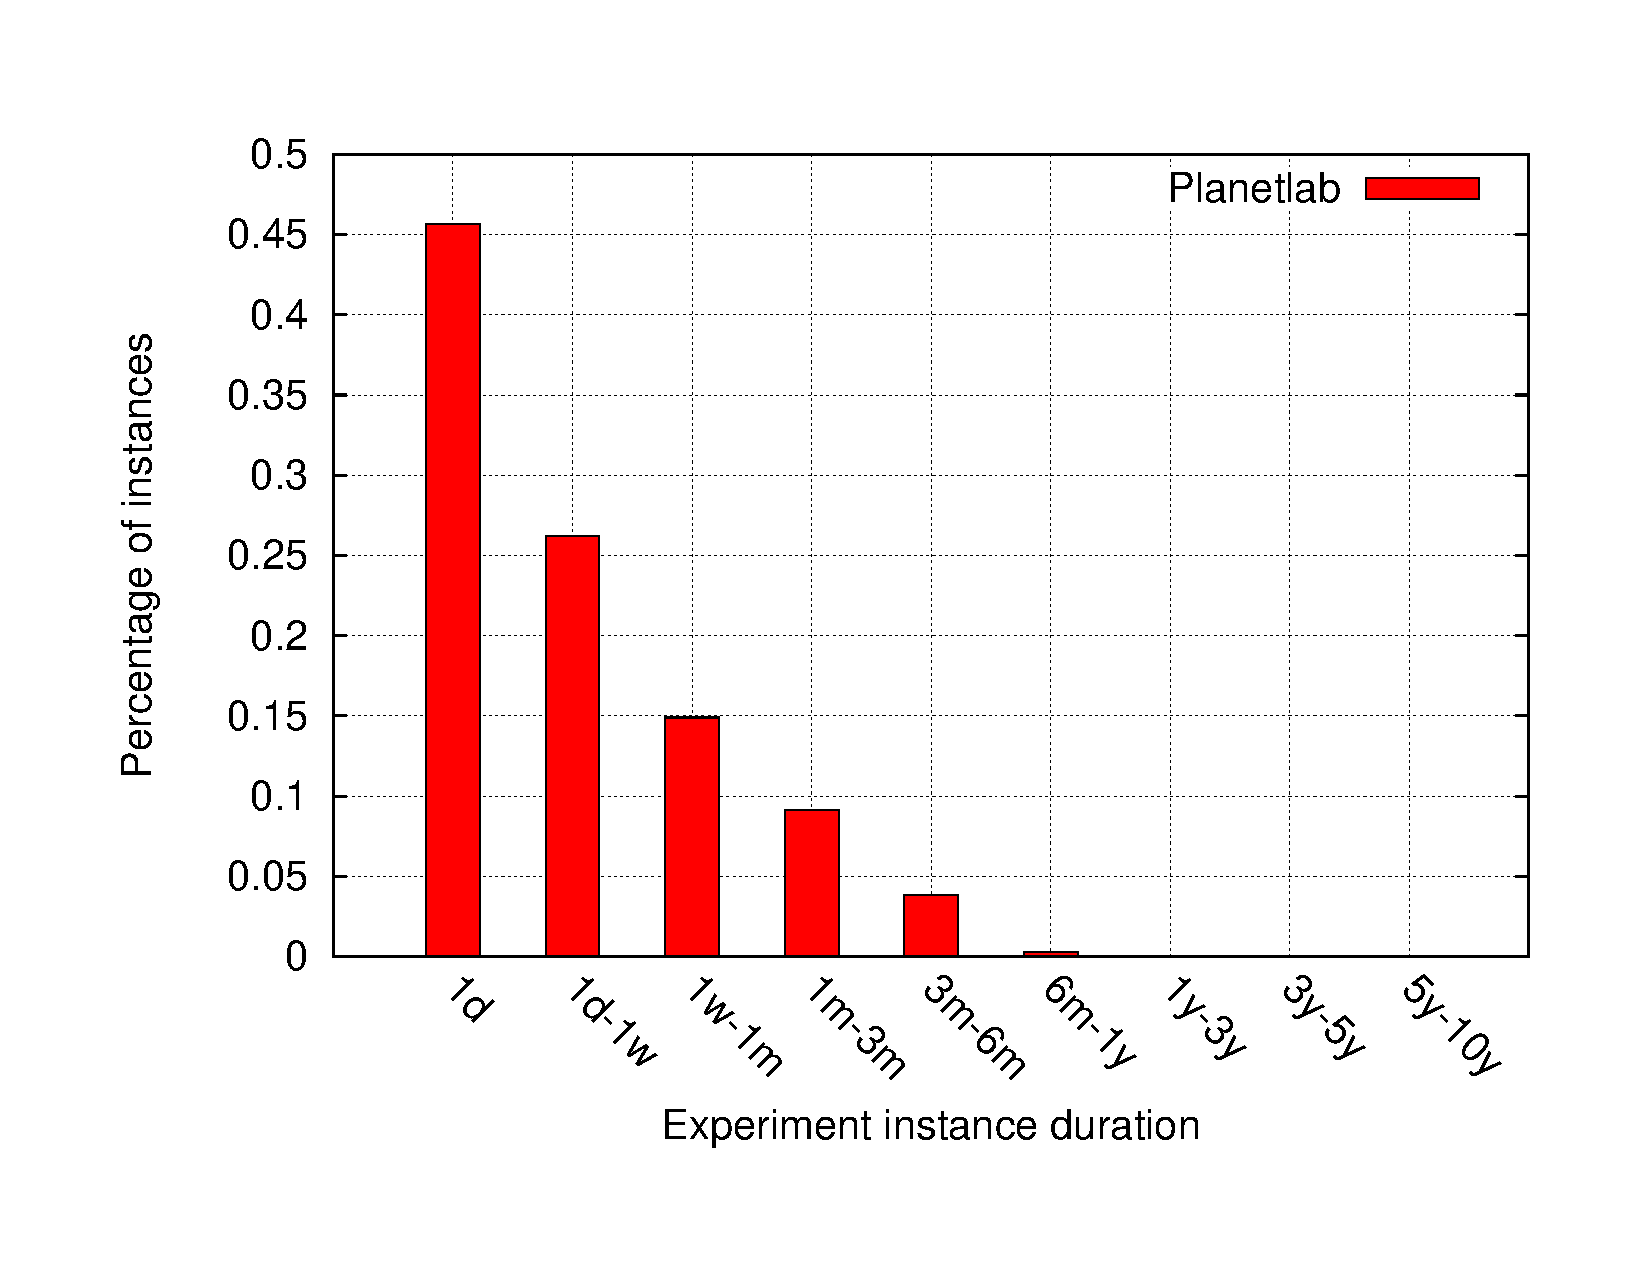
\includegraphics[width=3in,
type=pdf,ext=.pdf,read=.pdf]{figs/planet.dur.gnu} \caption{Experiment
instance duration in Planetlab} \label{expdur} \end{center} \end{figure}

\begin{figure}[htbp] \begin{center} 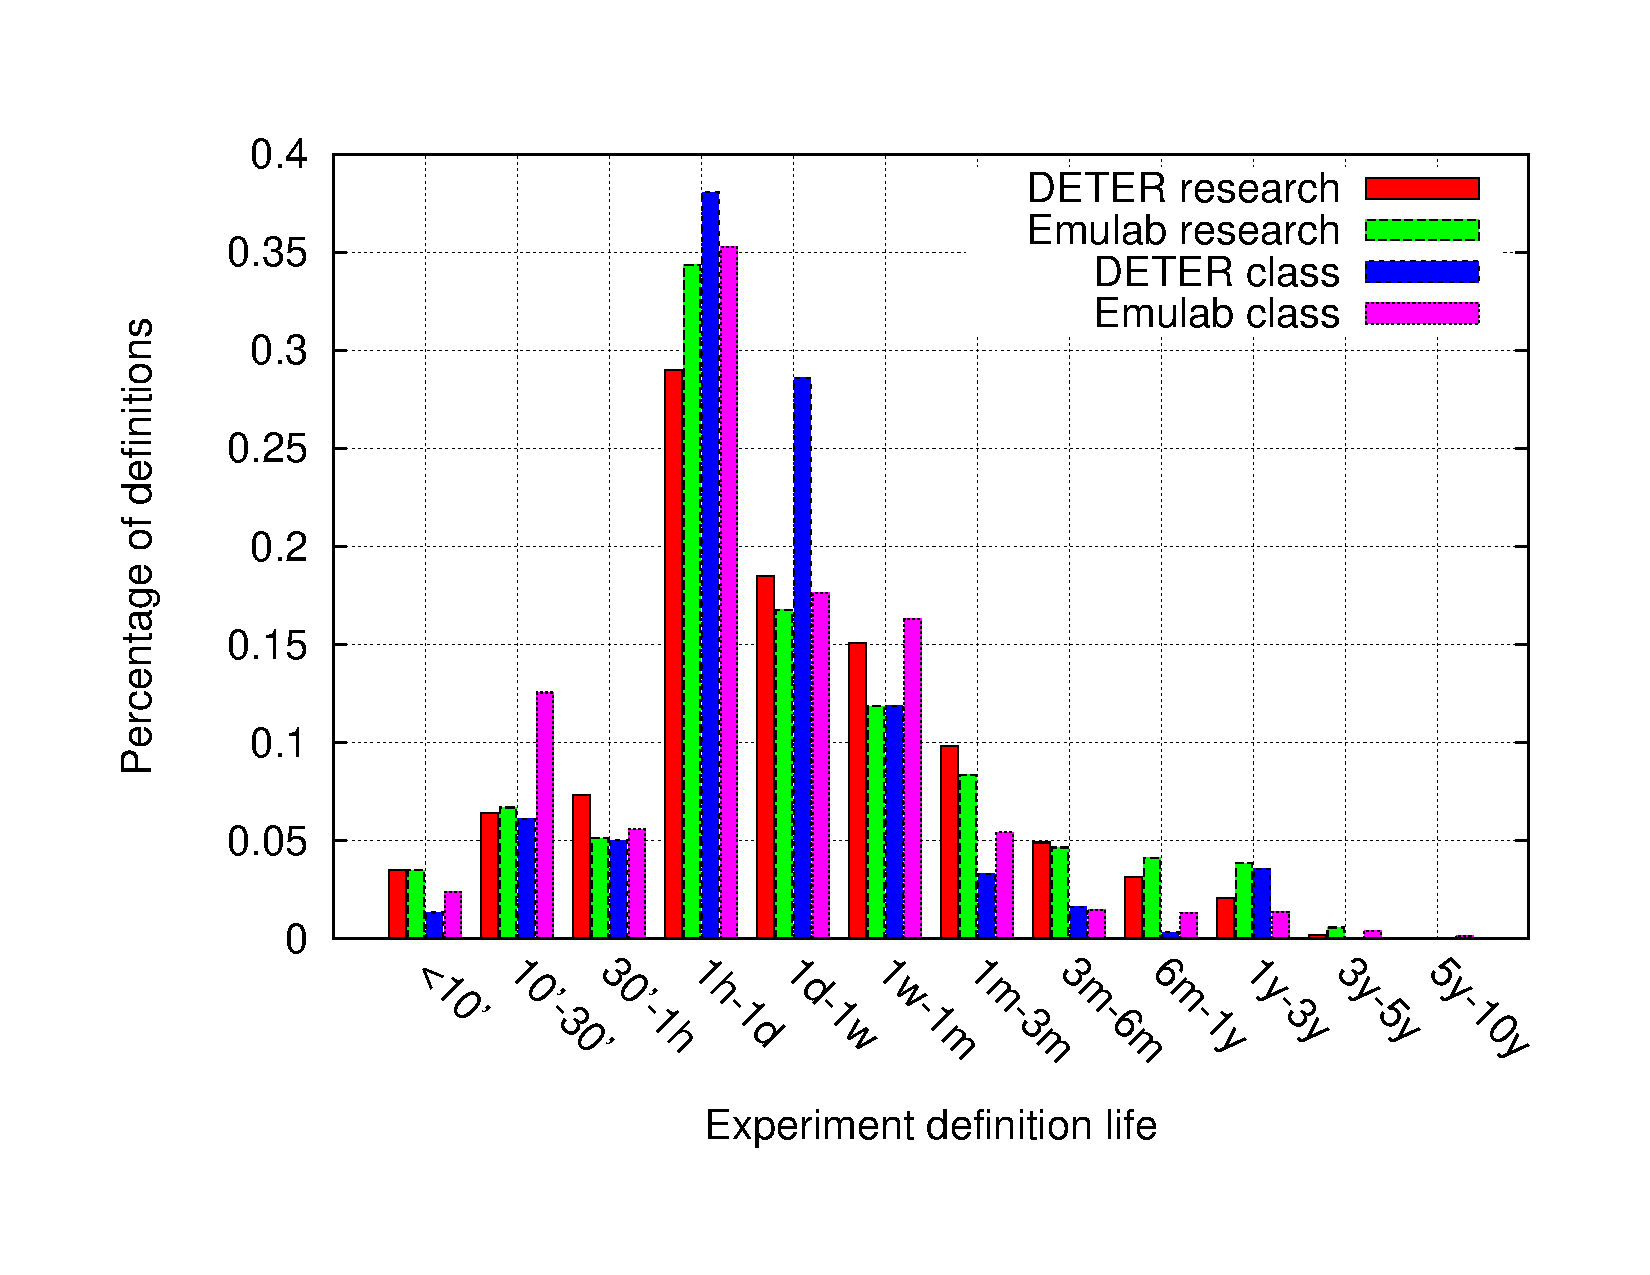
\includegraphics[width=3in,
type=pdf,ext=.pdf,read=.pdf]{figs/exp.life.gnu} \caption{Experiment
definition life} \label{explife} \end{center} \end{figure}

\begin{figure}[htbp] \begin{center} 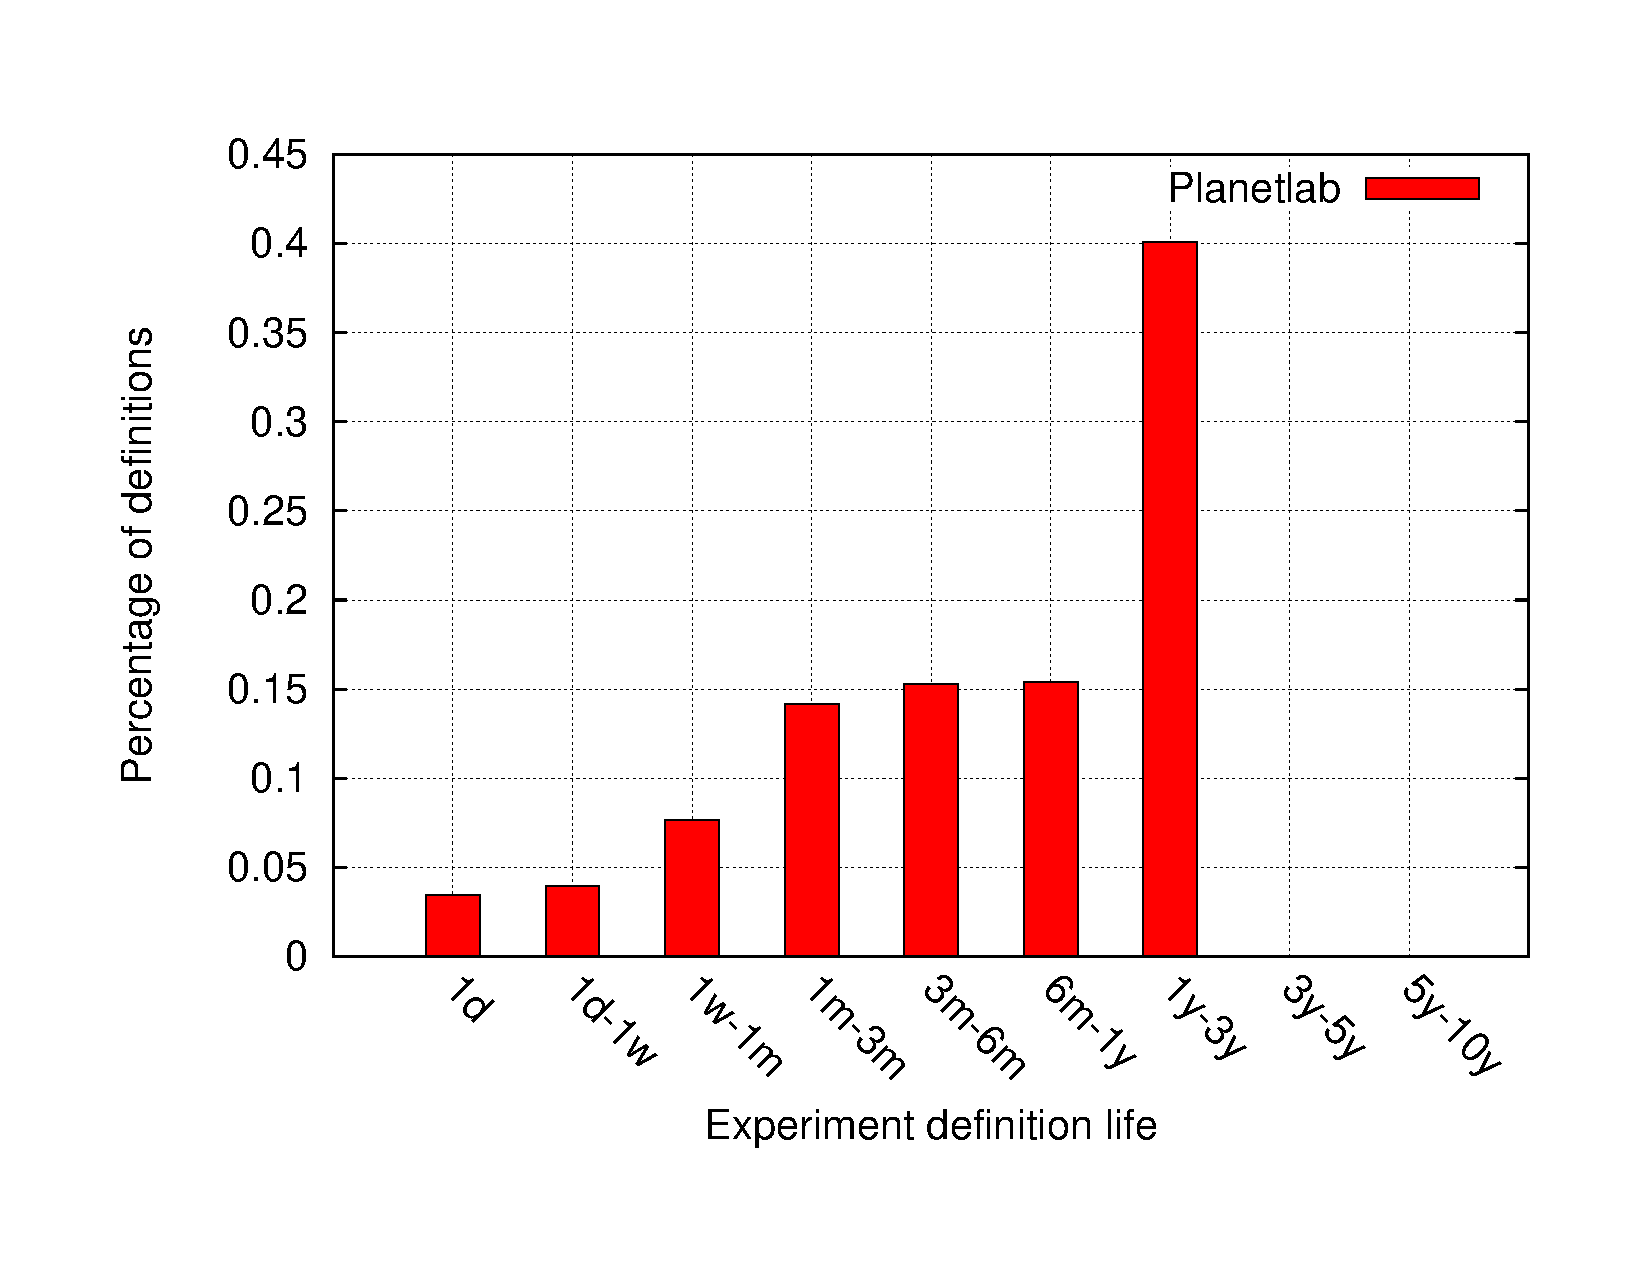
\includegraphics[width=3in,
type=pdf,ext=.pdf,read=.pdf]{figs/planet.life.gnu} \caption{Experiment
definition life in Planetlab} \label{explife} \end{center} \end{figure}

\begin{figure}[htbp] \begin{center} 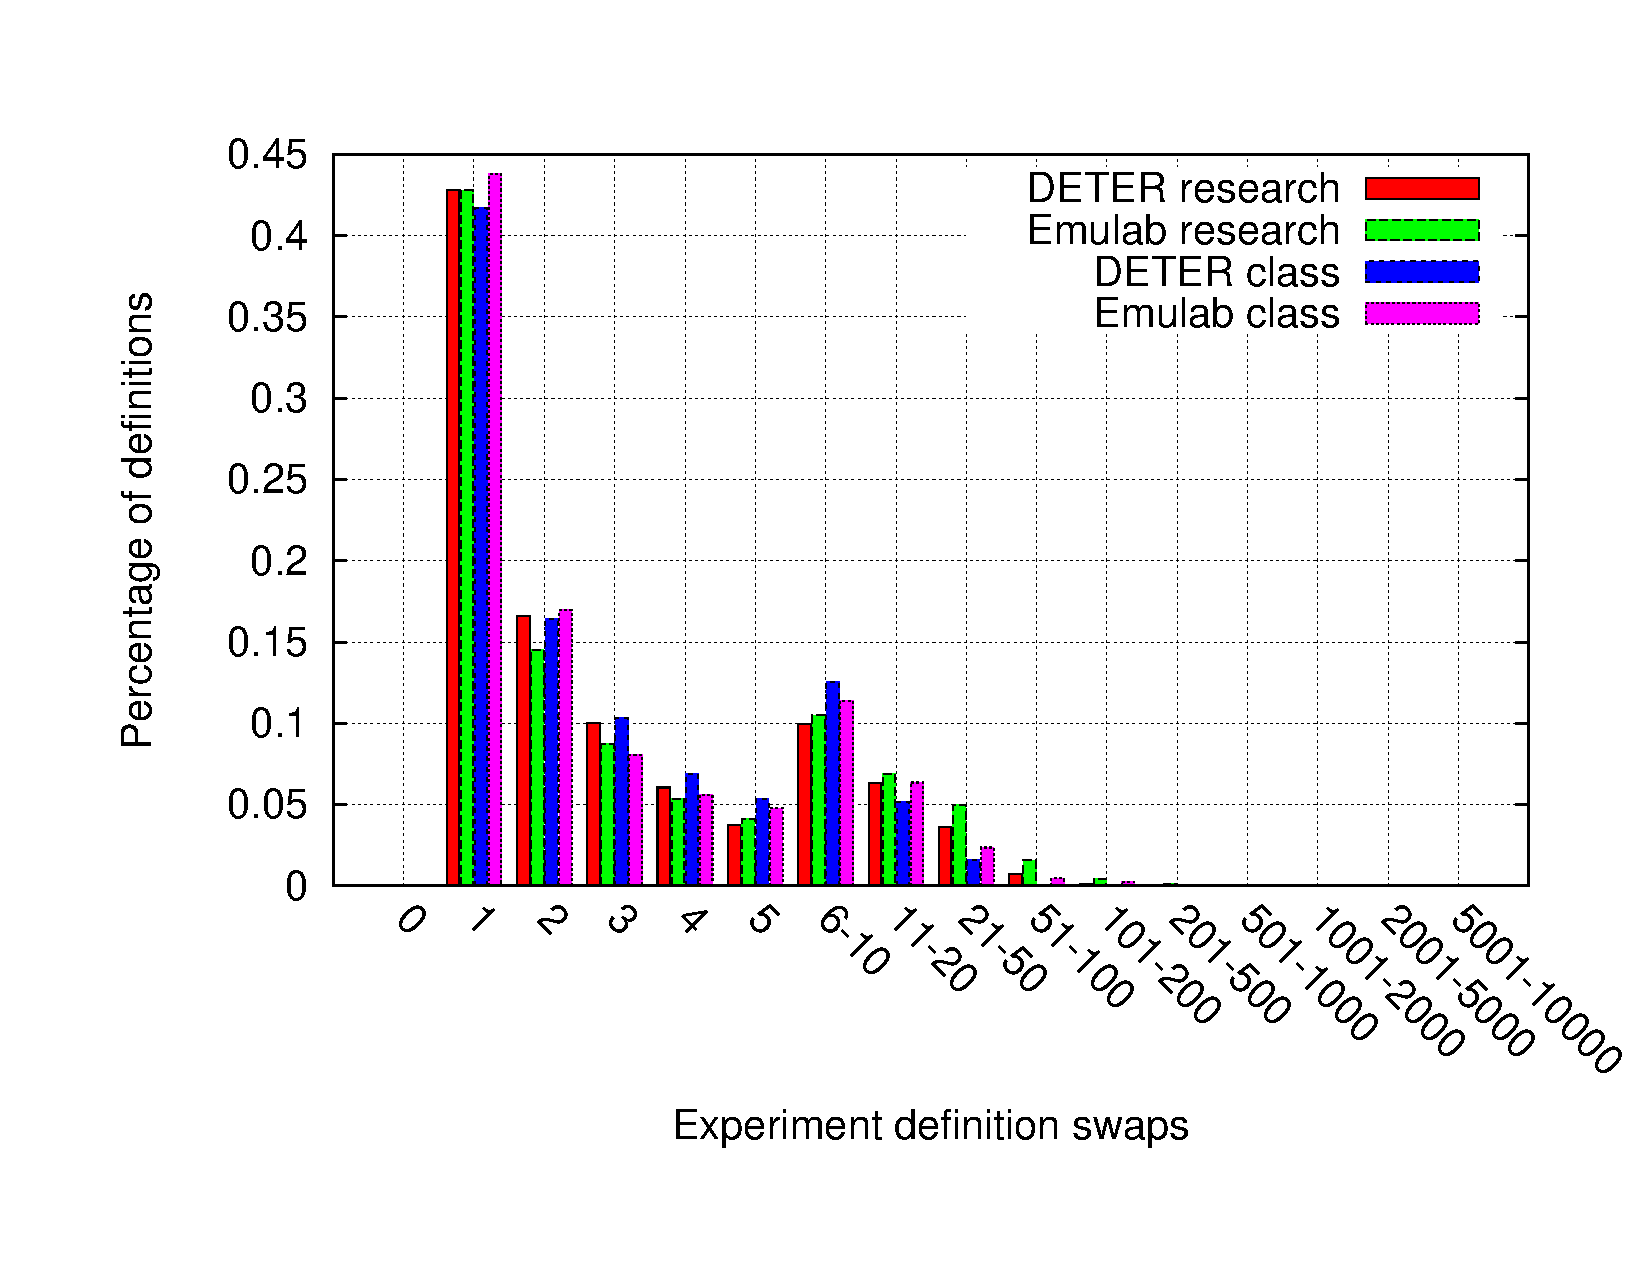
\includegraphics[width=3in,
type=pdf,ext=.pdf,read=.pdf]{figs/exp.swaps.gnu} \caption{Experiment
definition swaps} \label{expswaps} \end{center} \end{figure}

\begin{figure}[htbp] \begin{center} 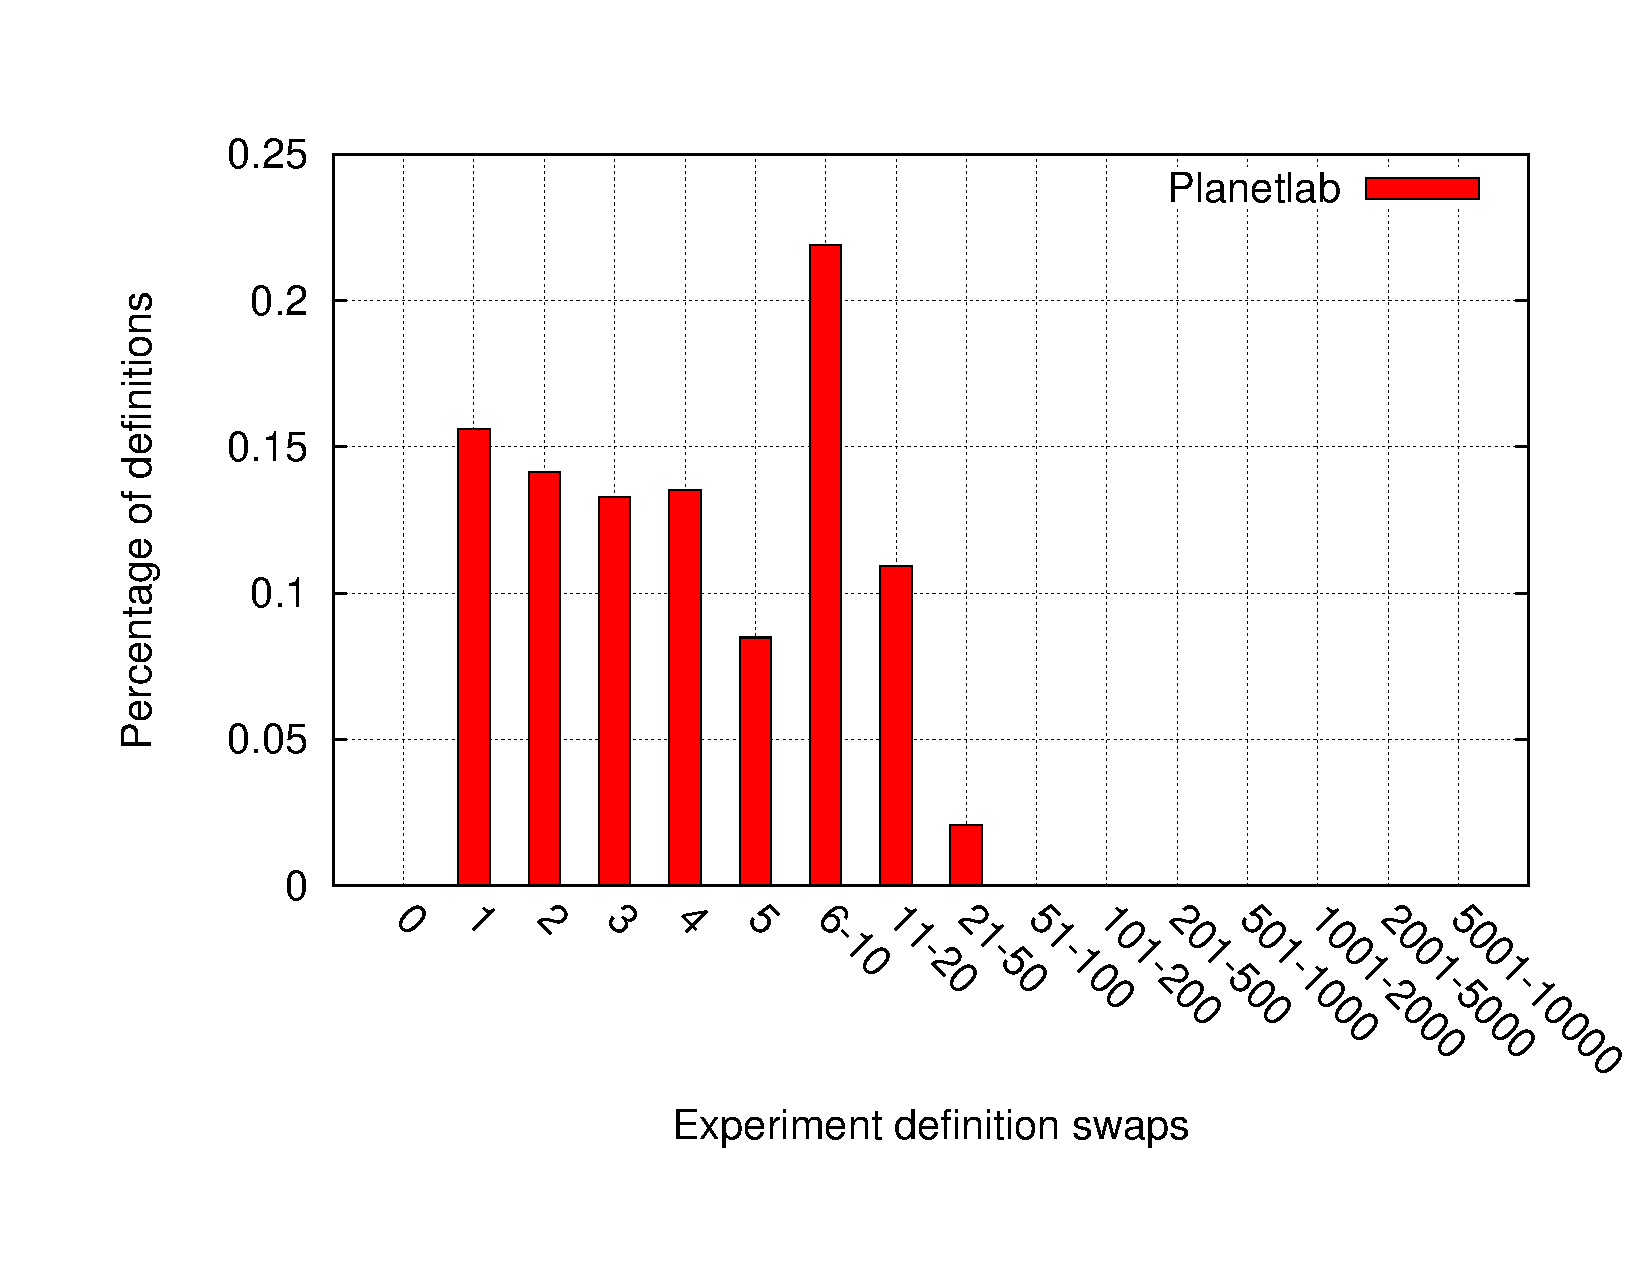
\includegraphics[width=3in,
type=pdf,ext=.pdf,read=.pdf]{figs/planet.swaps.gnu} \caption{Experiment
definition swaps in Planetlab} \label{expswaps} \end{center}
\end{figure}

\begin{figure*}[htbp] \begin{center} 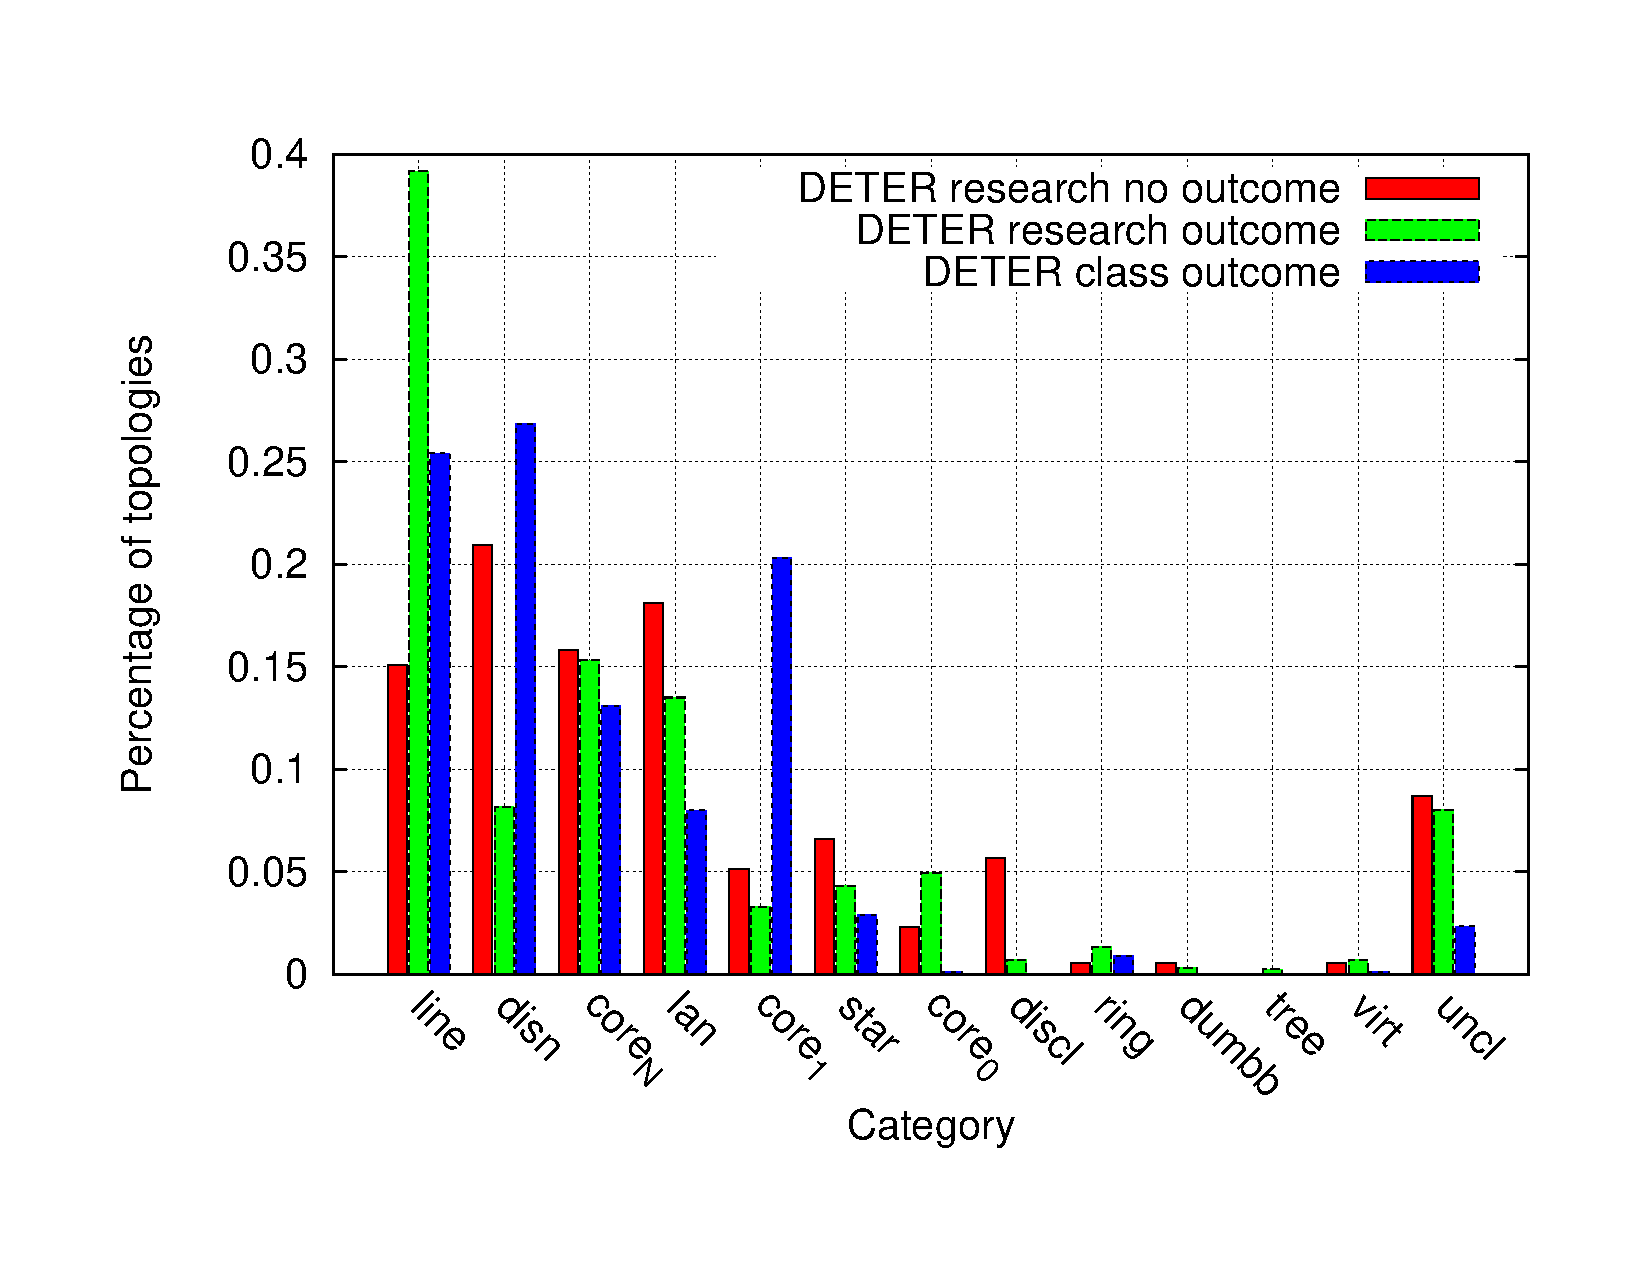
\includegraphics[width=3in,
type=pdf,ext=.pdf,read=.pdf]{figs/topo.gnu} 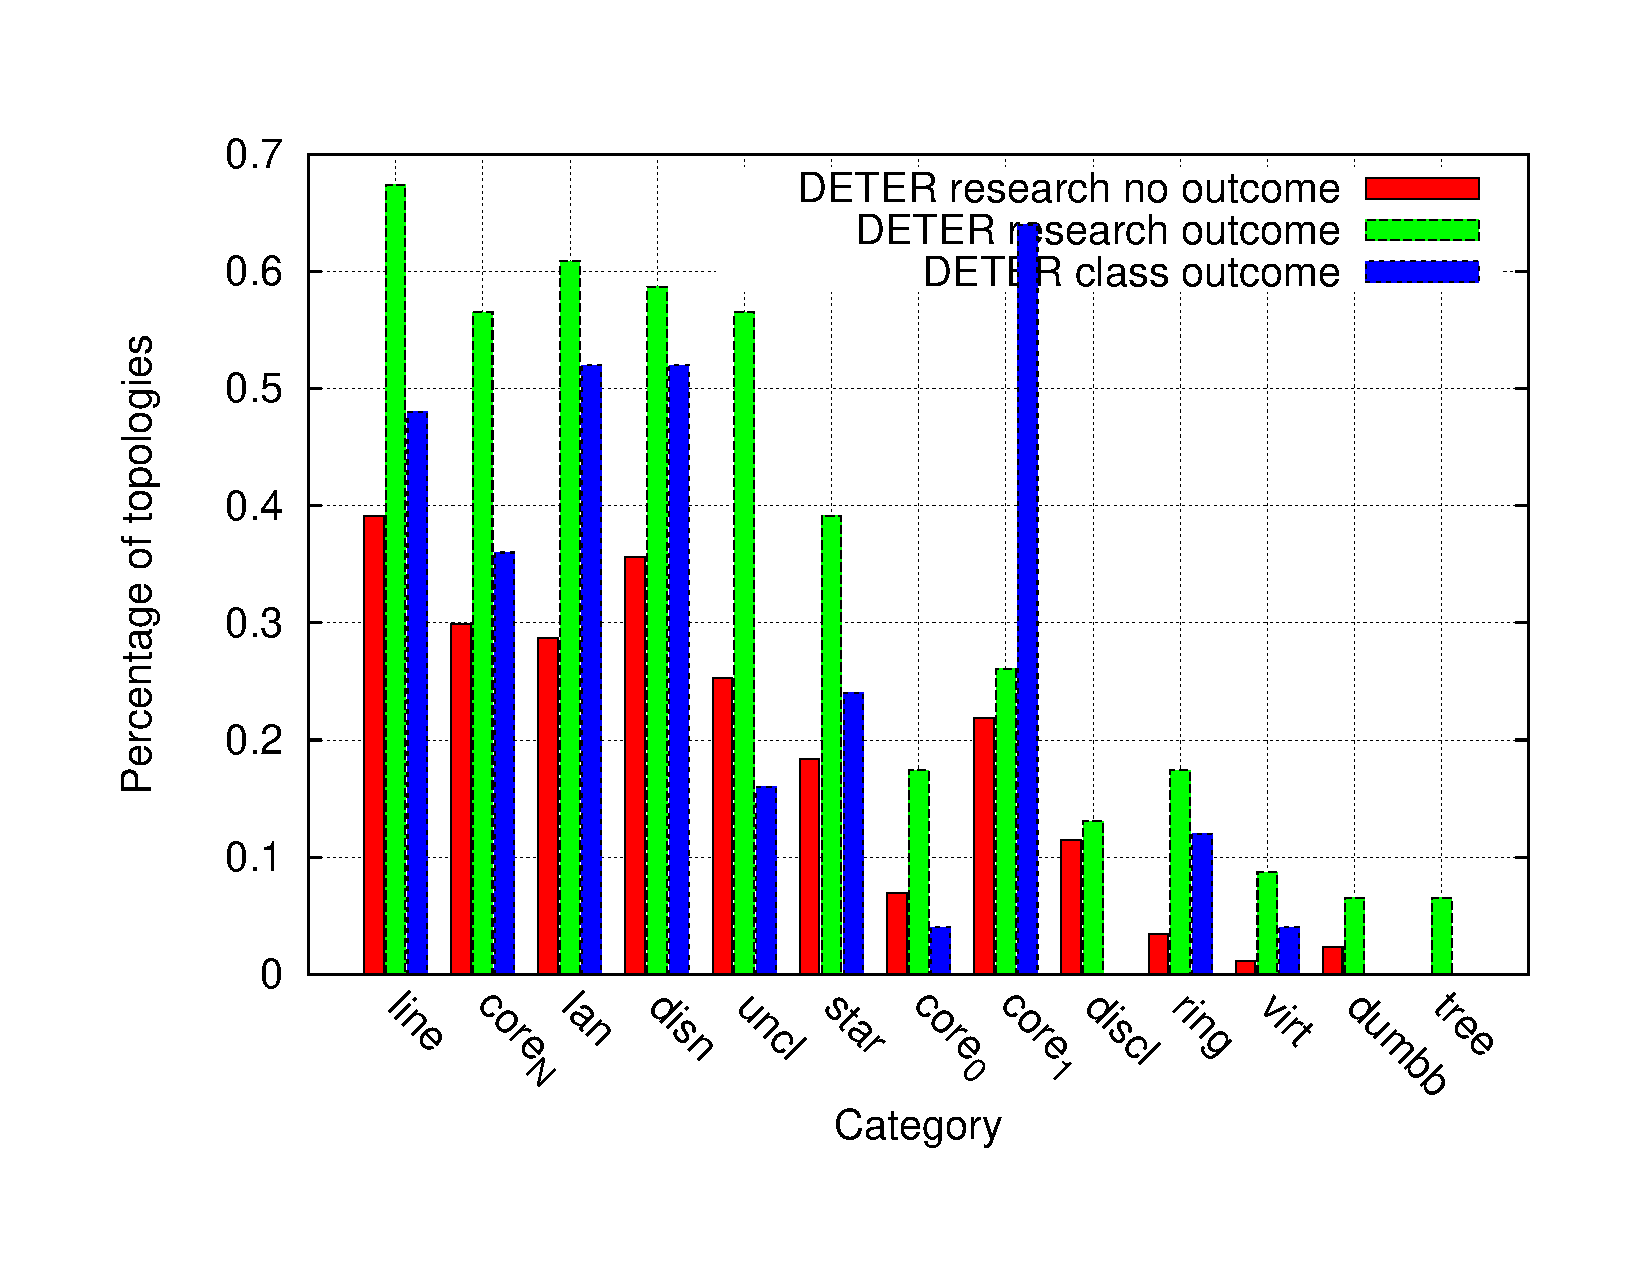
\includegraphics[width=3in,
type=pdf,ext=.pdf,read=.pdf]{figs/topop.gnu} \caption{Experiment
topologies in DETER: experiment vs project distribution} \label{topo}
\end{center} \end{figure*}



\subsection{Project Distributions} 

In this case trends differ between all and outcome projects. Those with
outcome are definitely more active. \begin{figure*}[htbp] \begin{center}
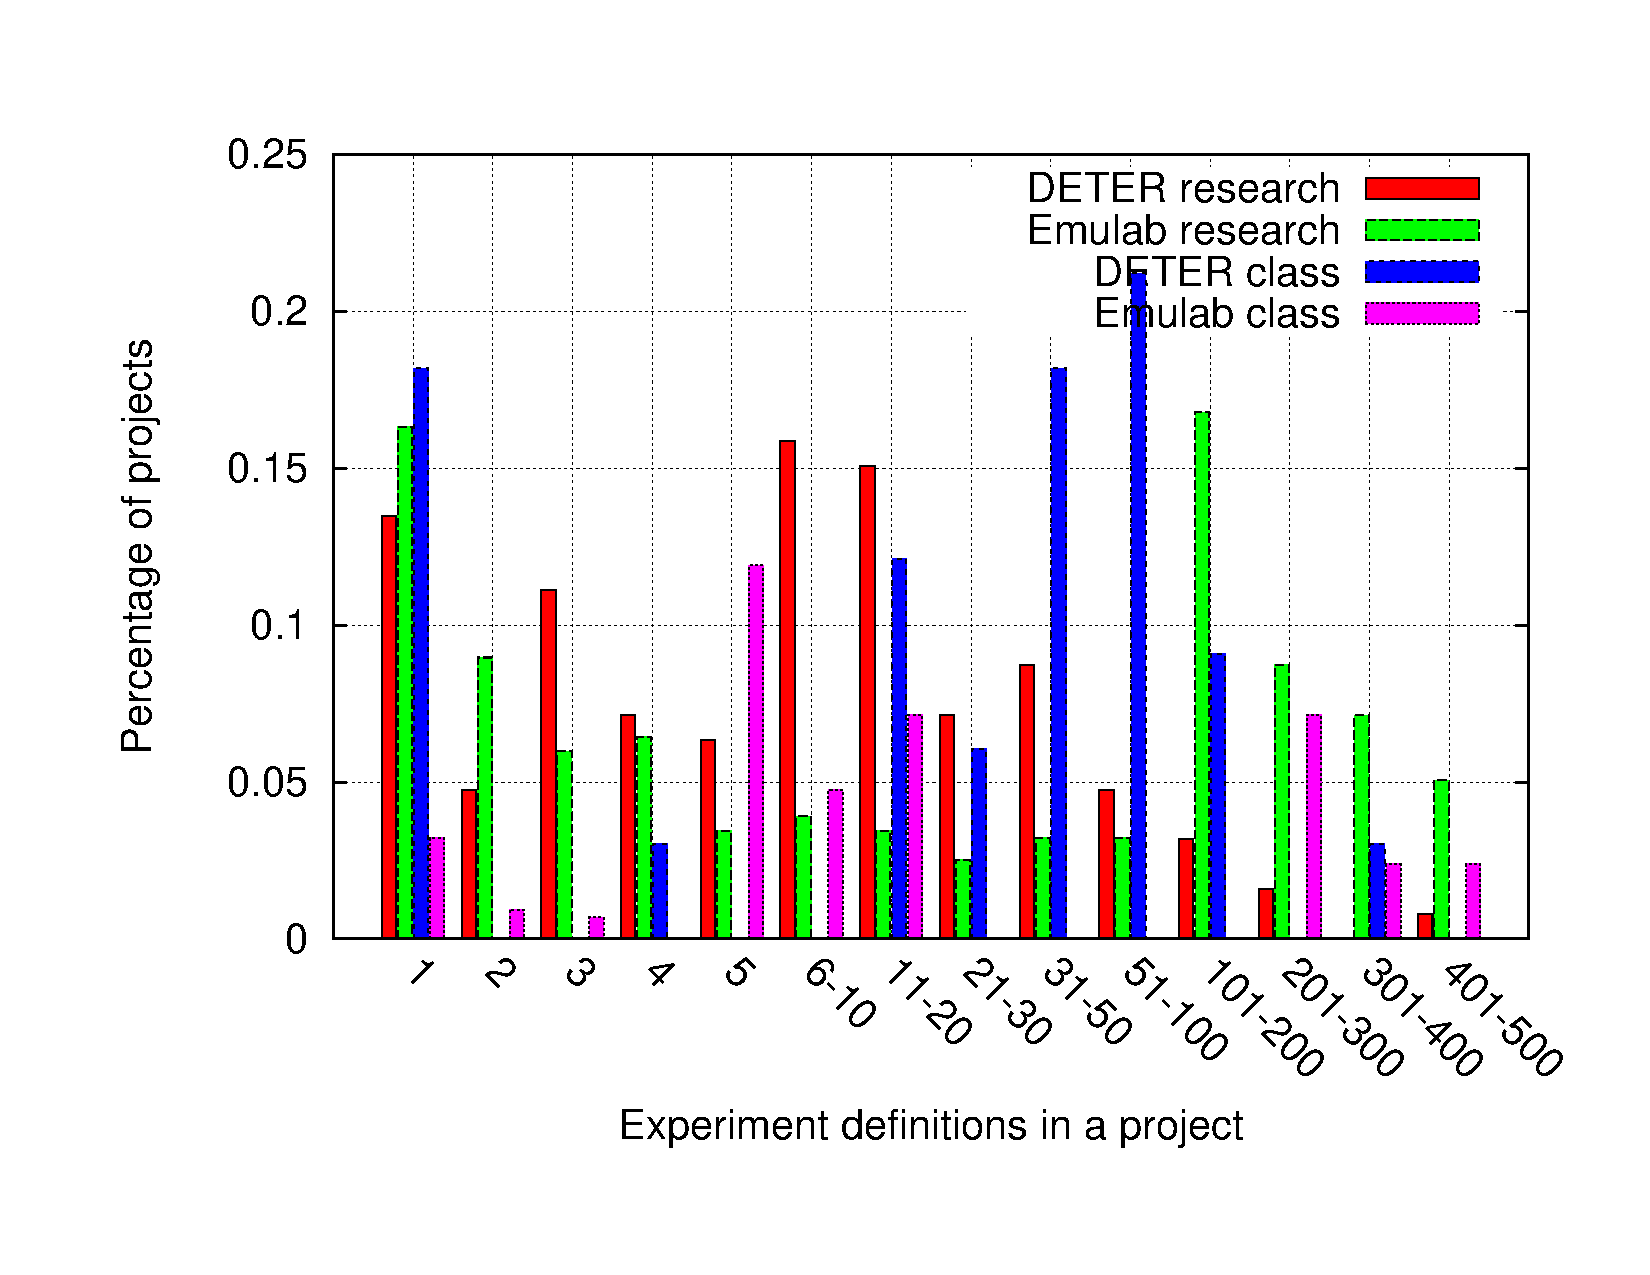
\includegraphics[width=3in,
type=pdf,ext=.pdf,read=.pdf]{figs/proj.size.gnu}
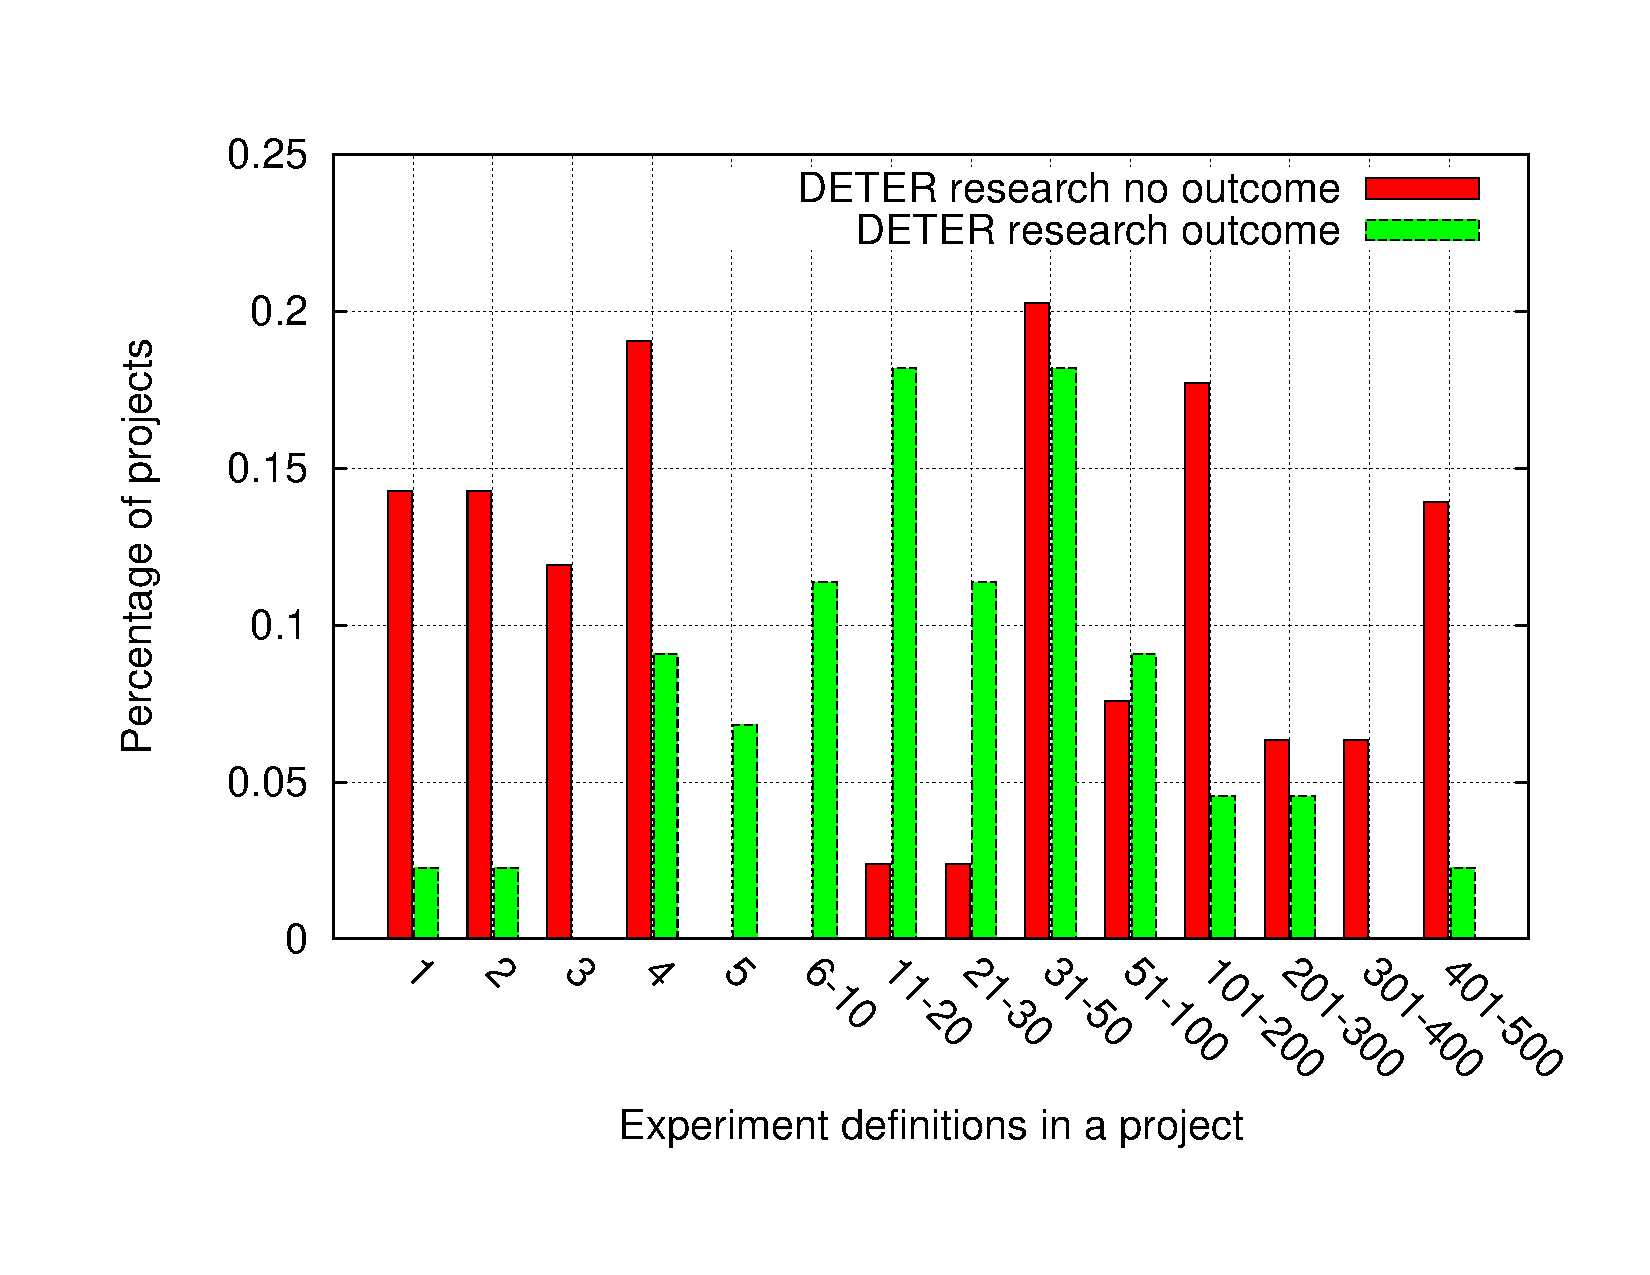
\includegraphics[width=3in,
type=pdf,ext=.pdf,read=.pdf]{figs/proj.size.cmp.gnu}
\caption{Experiments per project. Left: DETER vs Emulab, Right: All vs
outcome} \label{projsize} \end{center} \end{figure*}

\begin{figure*}[htbp] \begin{center} 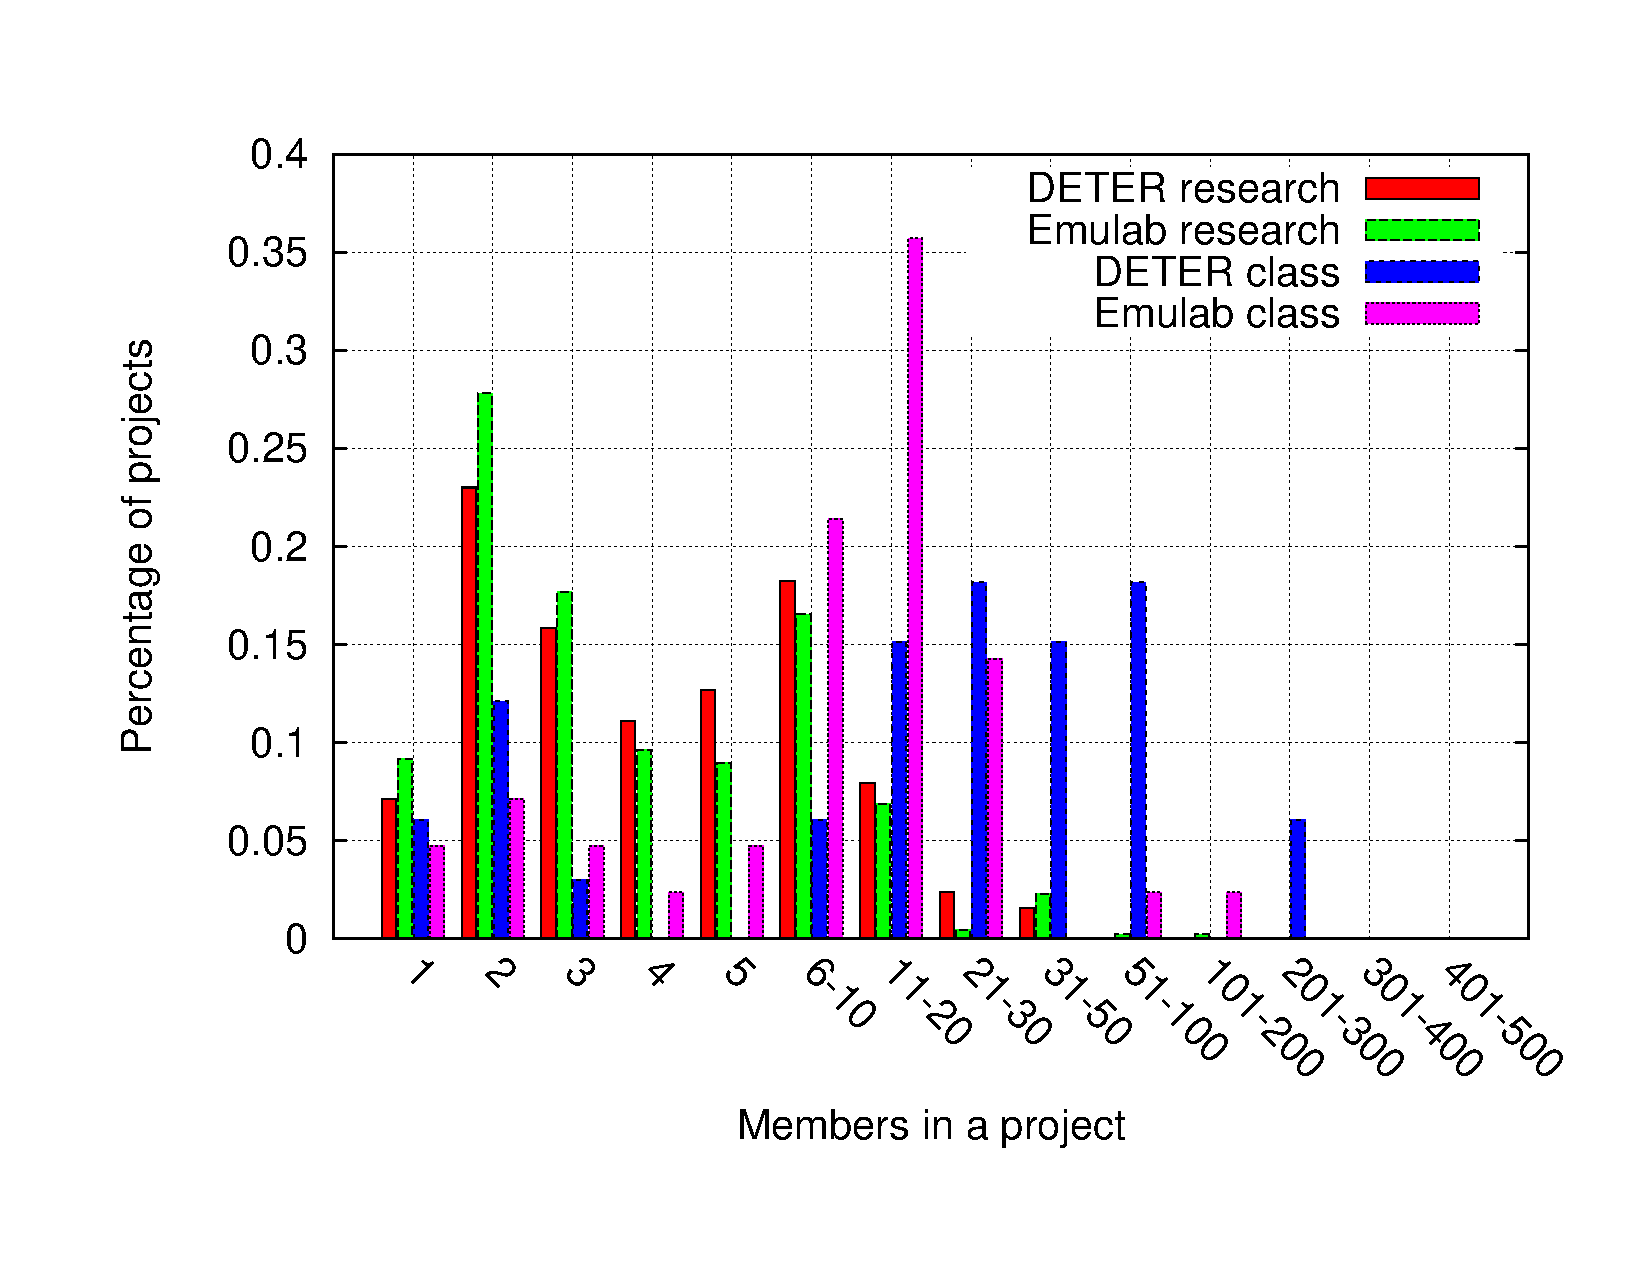
\includegraphics[width=3in,
type=pdf,ext=.pdf,read=.pdf]{figs/proj.user.gnu}
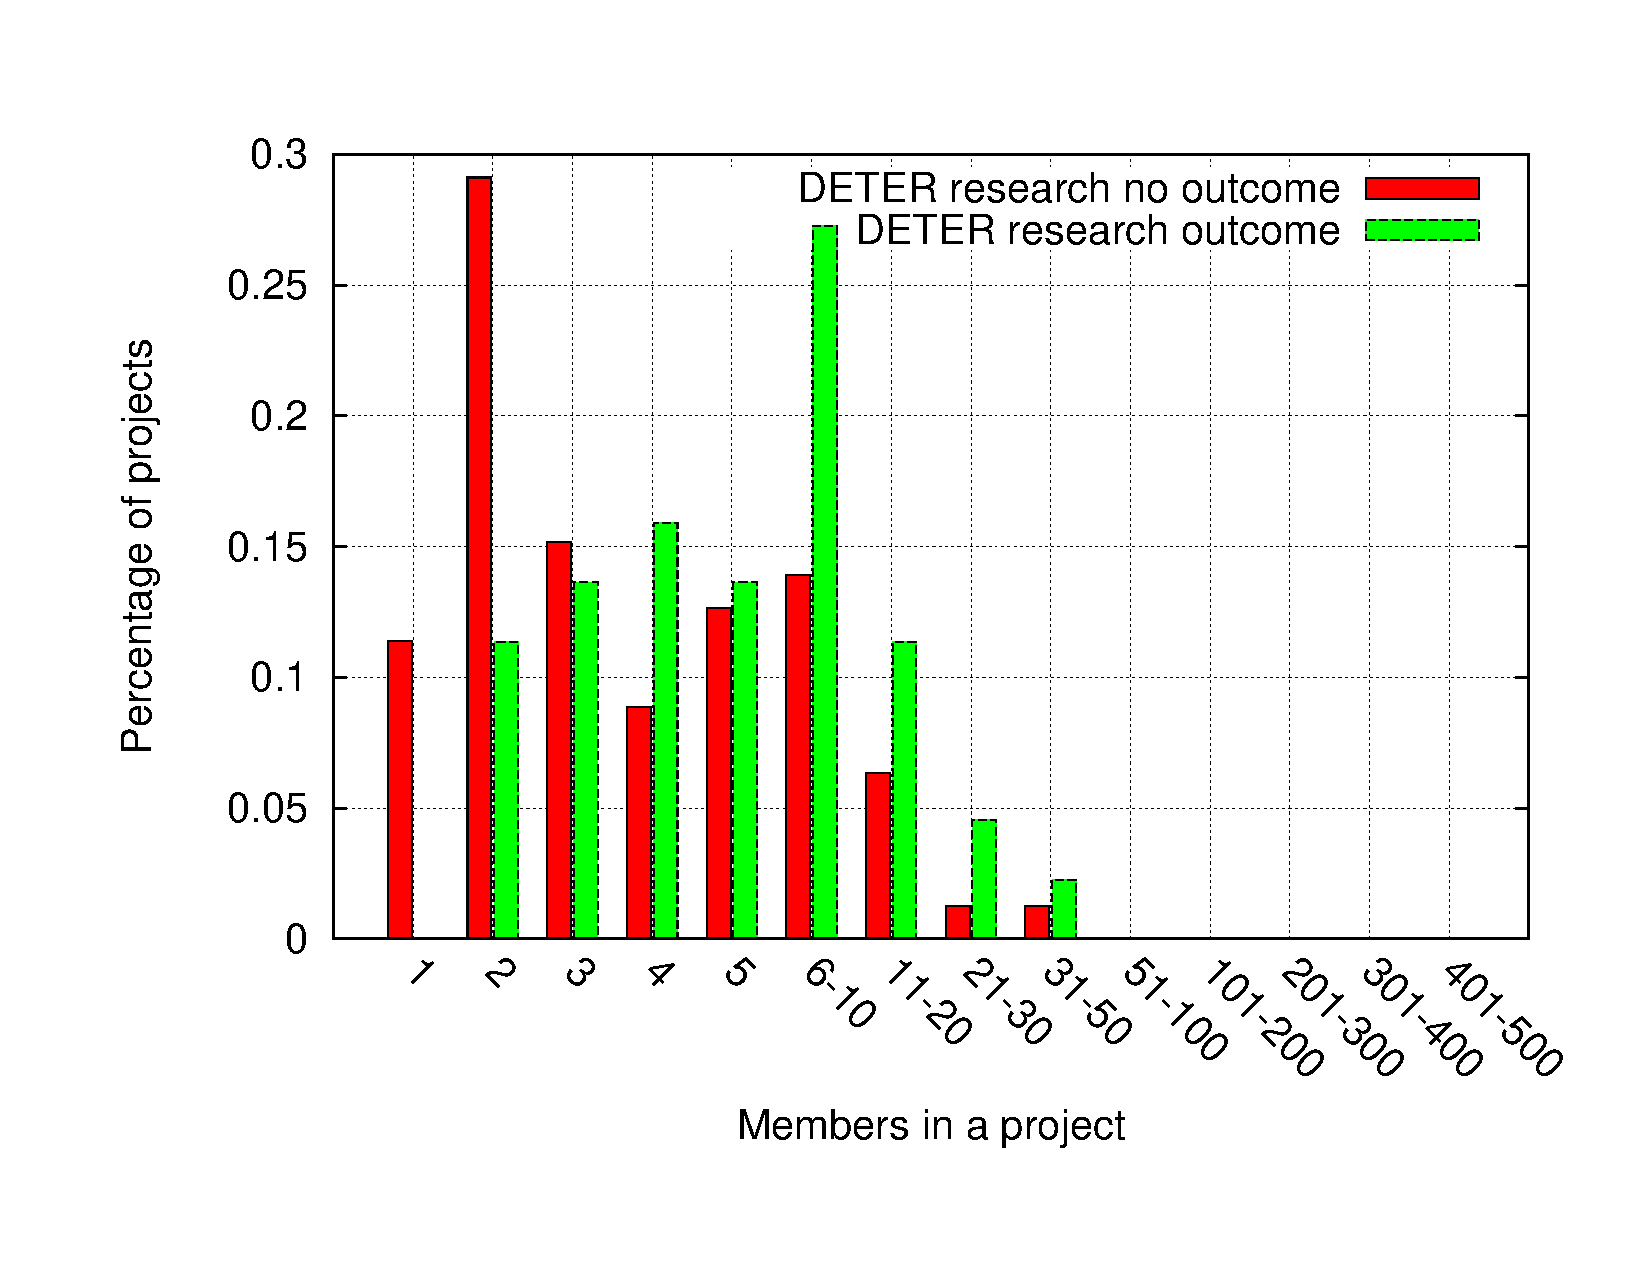
\includegraphics[width=3in,
type=pdf,ext=.pdf,read=.pdf]{figs/proj.user.cmp.gnu} \caption{Members
per project. Left: DETER vs Emulab, Right: All vs outcome}
\label{projuser} \end{center} \end{figure*}

\begin{figure*}[htbp] \begin{center} 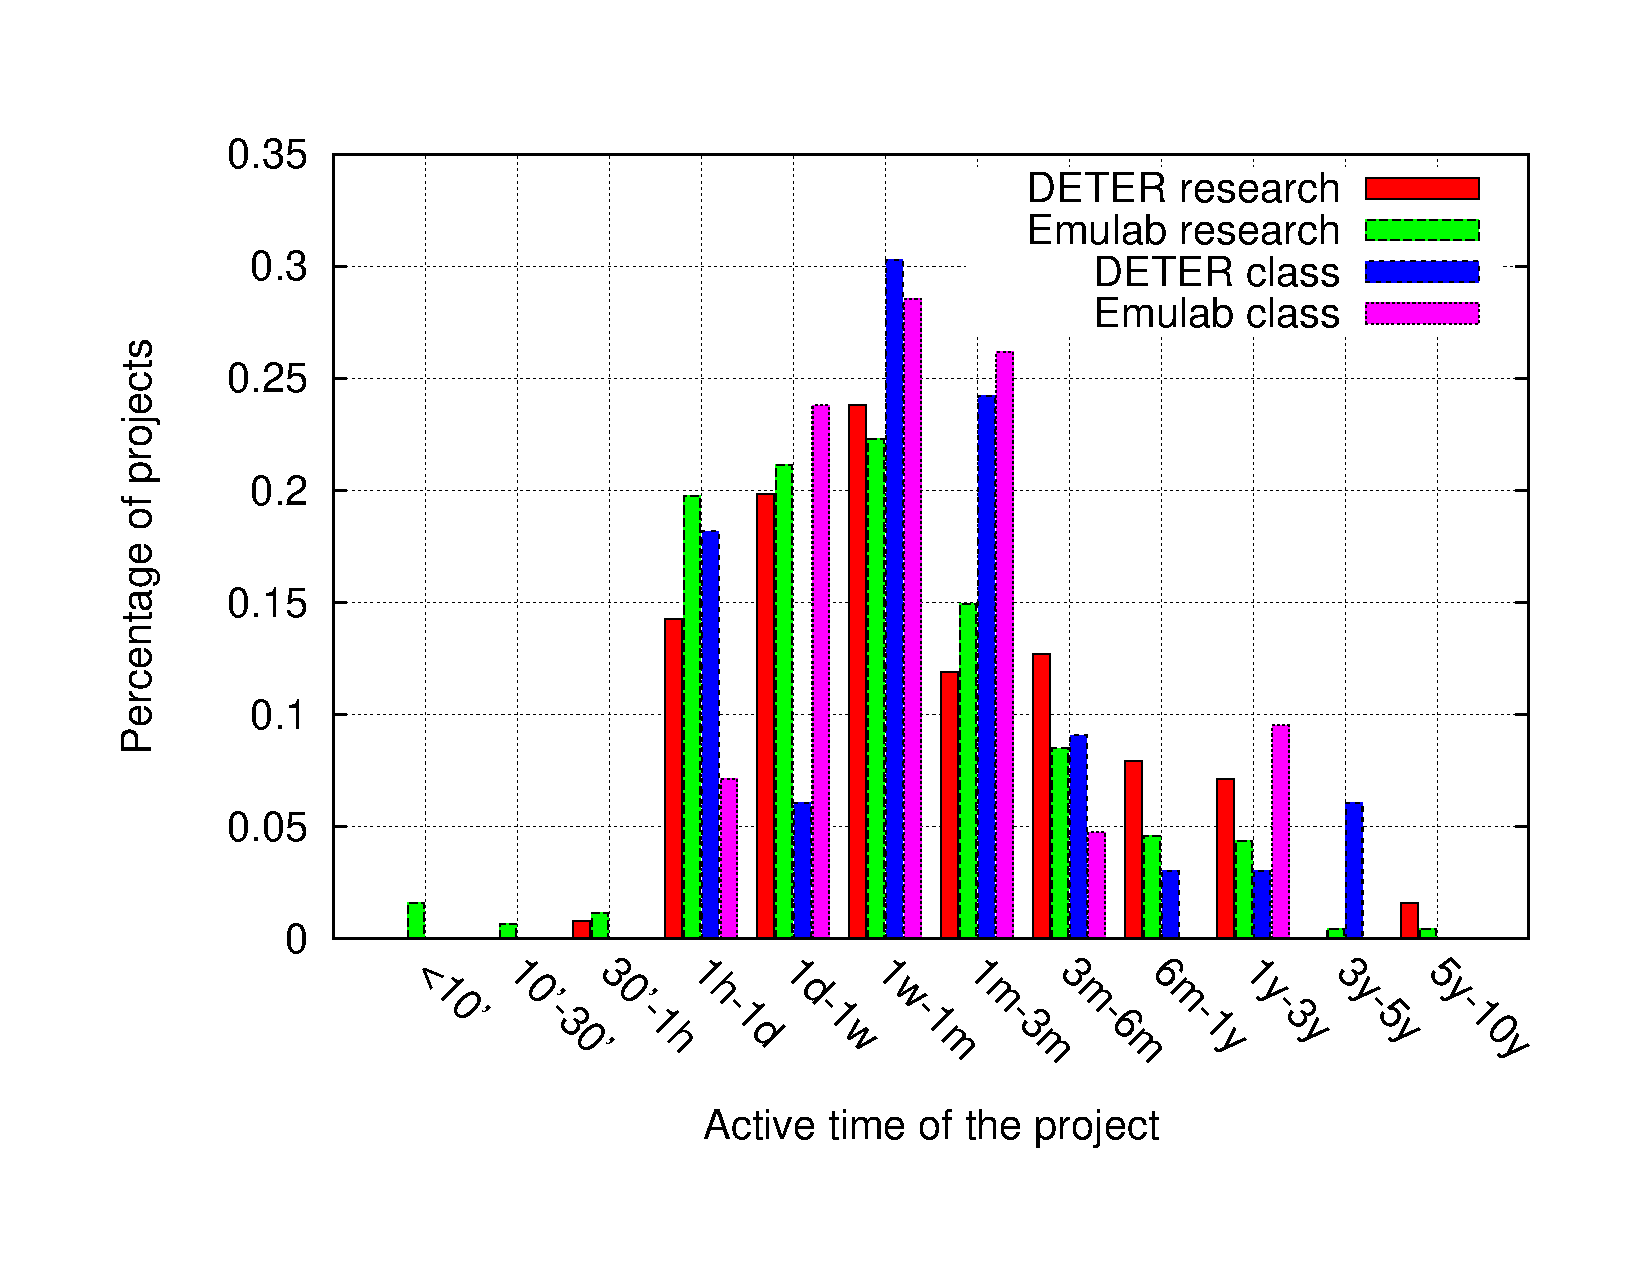
\includegraphics[width=3in,
type=pdf,ext=.pdf,read=.pdf]{figs/proj.active.gnu}
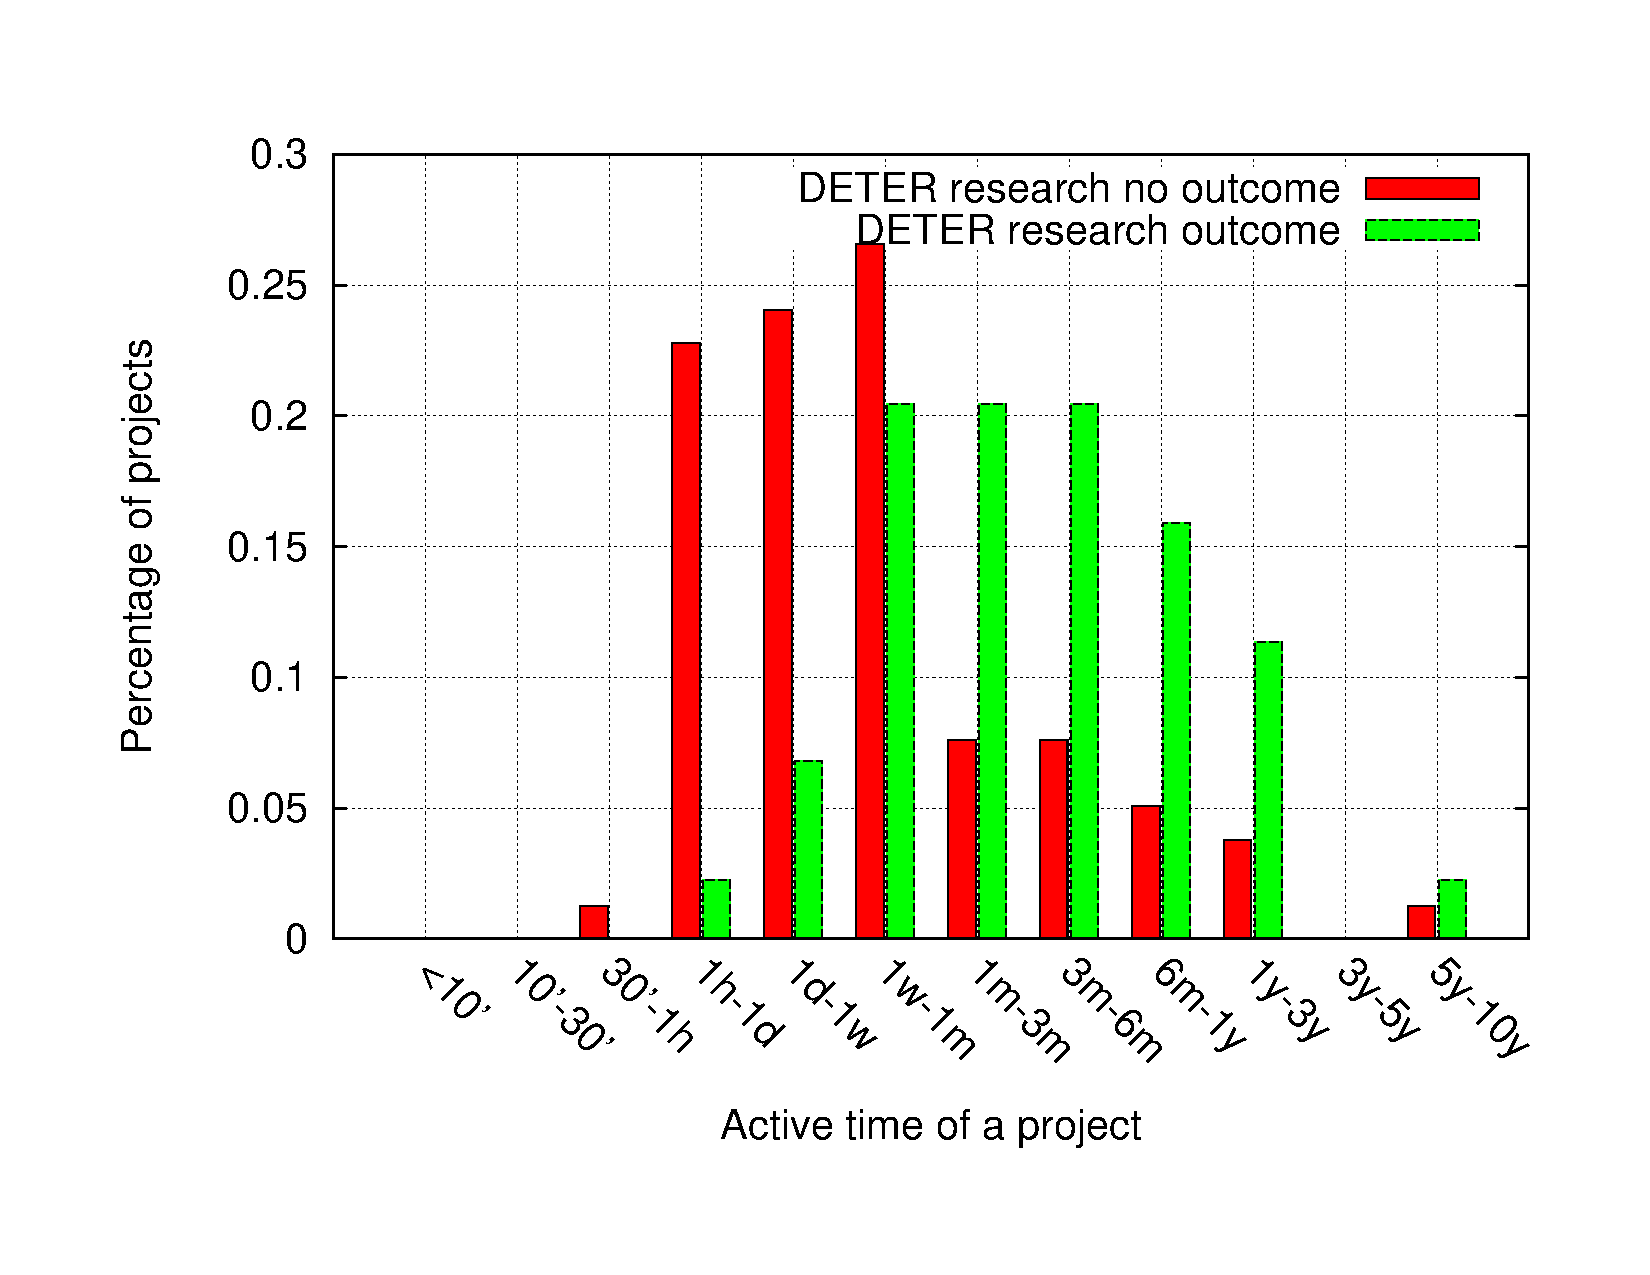
\includegraphics[width=3in,
type=pdf,ext=.pdf,read=.pdf]{figs/proj.active.cmp.gnu} \caption{Active
time of a project. Left: DETER vs Emulab, Right: All vs outcome}
\label{projactive} \end{center} \end{figure*}


\begin{figure*}[htbp] \begin{center} 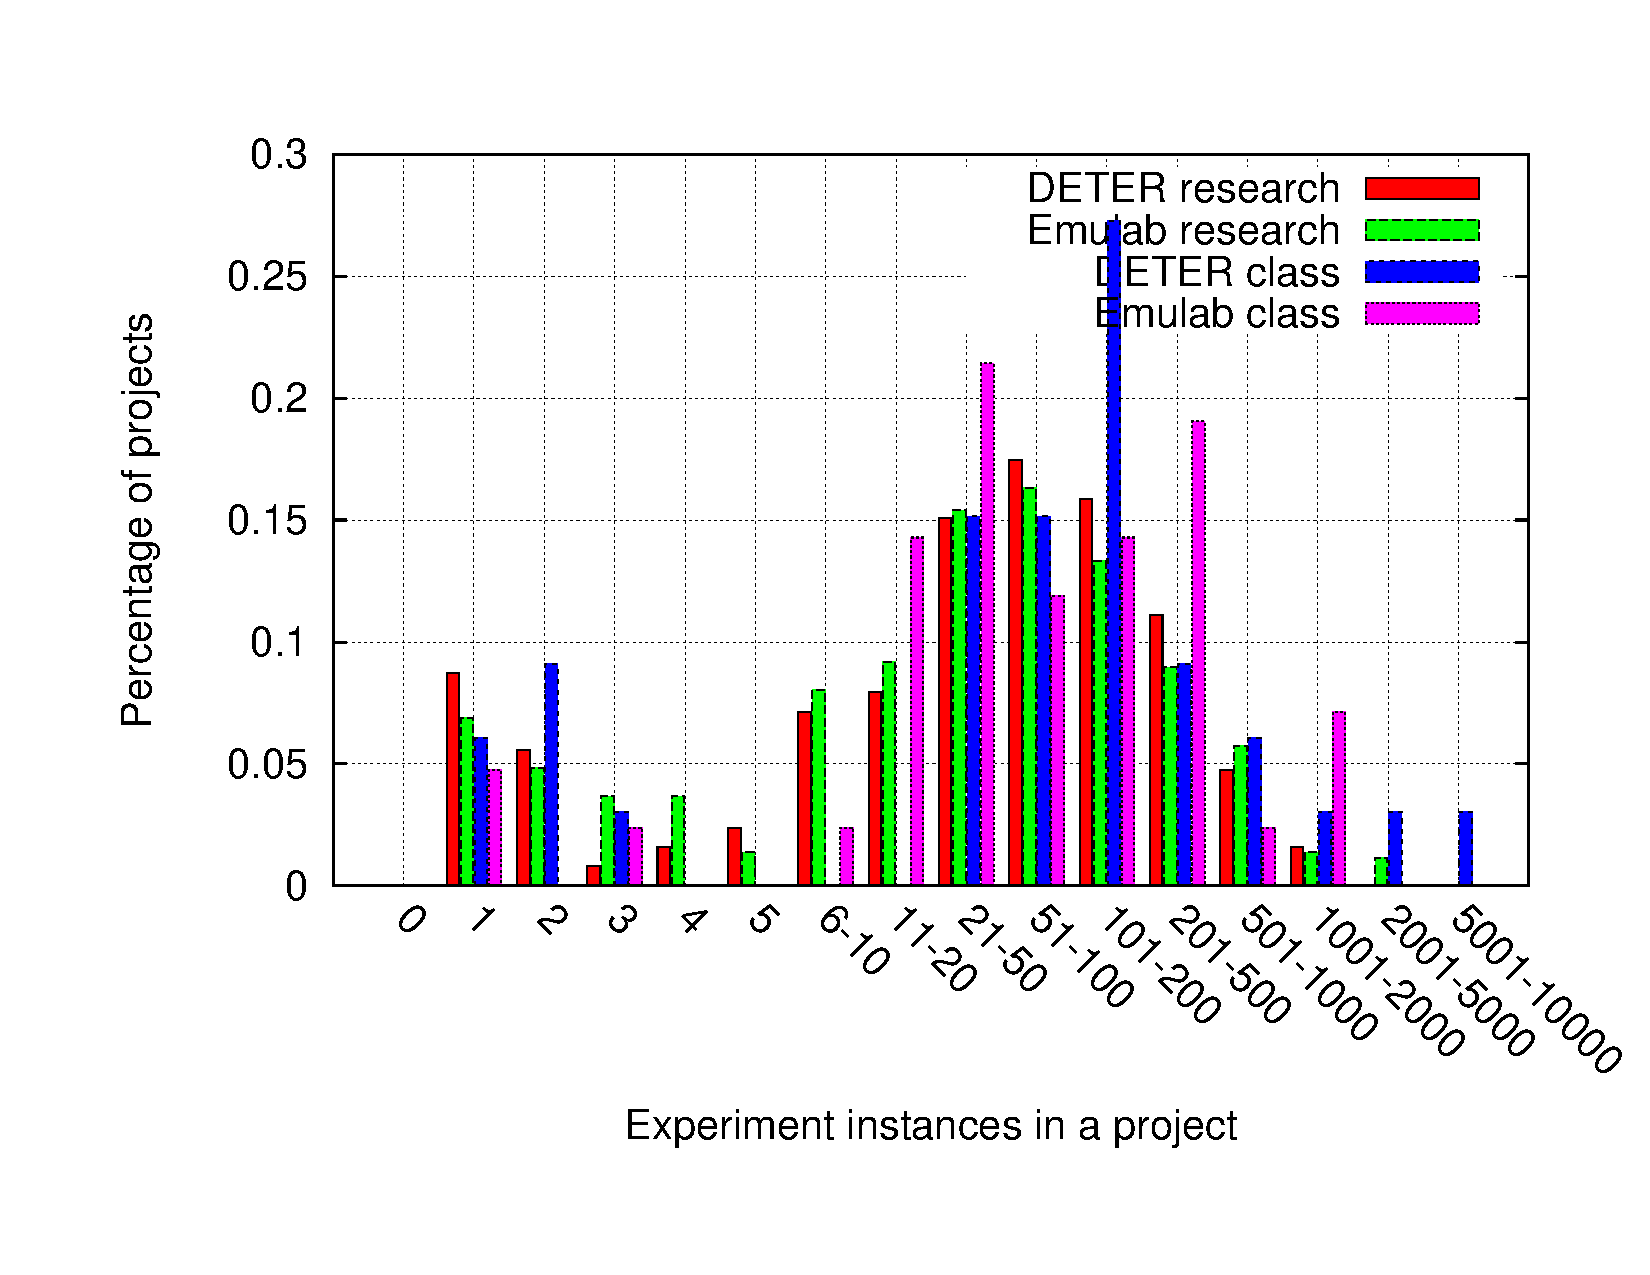
\includegraphics[width=3in,
type=pdf,ext=.pdf,read=.pdf]{figs/proj.swaps.gnu}
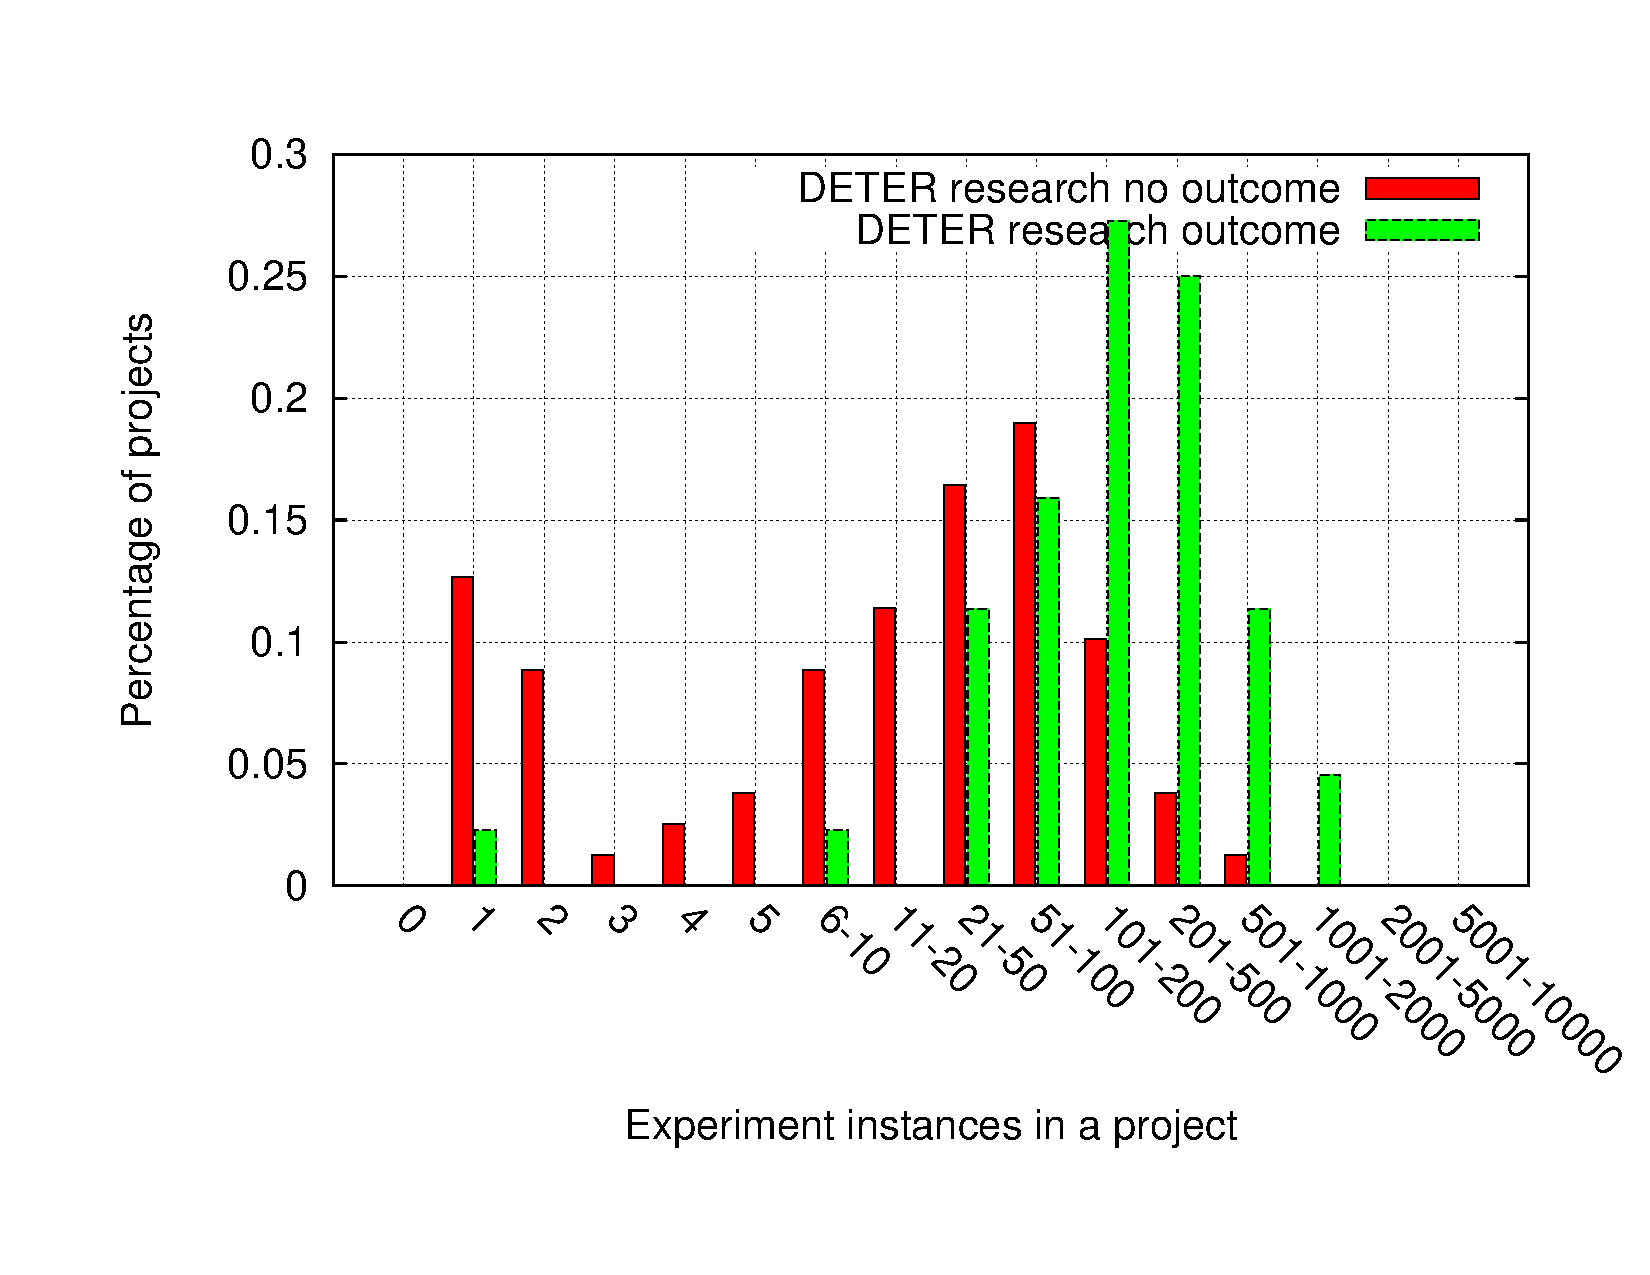
\includegraphics[width=3in,
type=pdf,ext=.pdf,read=.pdf]{figs/proj.swaps.cmp.gnu}
\caption{Experiment instances in a project. Left: DETER vs Emulab,
Right: All vs outcome} \label{projswaps} \end{center} \end{figure*}

Are outcome projects more active because they have been around longer or
because they work harder? Both. Figure \ref{projagevsactive} shows that.
Figure \ref{projuservsauser} shows that in large research projects with
outcome almost all users are active, while in smaller projects only a
few may be active. What's surprising is that for classes with outcome
sometimes only half of the users are active. This may be due to them
having a choice of using DETER vs not or maybe because we create more
accounts than needed for the class.

\begin{figure*}[htbp] \begin{center} \includegraphics[width=3in,
type=pdf,ext=.pdf,read=.pdf]{figs/proj.agevsactive.res.gnu}
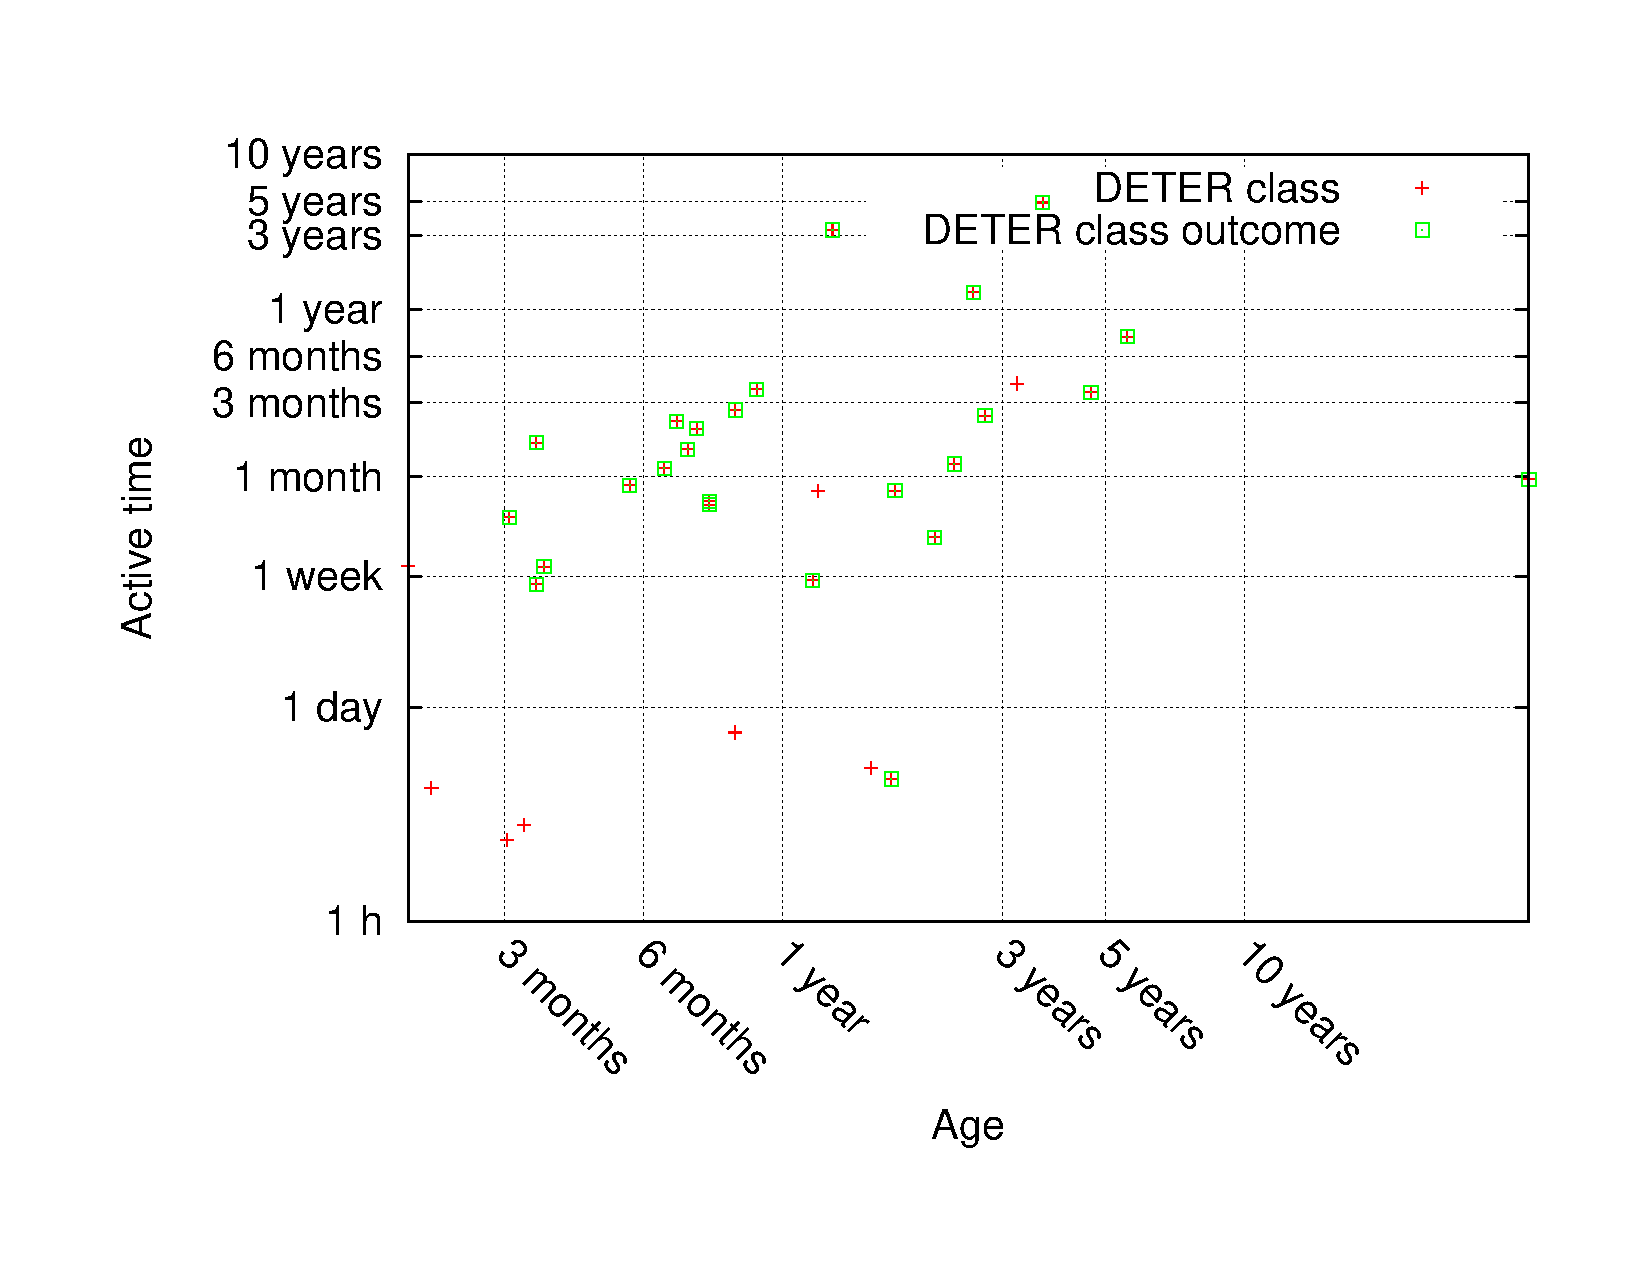
\includegraphics[width=3in,
type=pdf,ext=.pdf,read=.pdf]{figs/proj.agevsactivecl.gnu}
\caption{Active time vs age of a project. Left: DETER research, right:
DETER class} \label{projagevsactive} \end{center} \end{figure*}

\begin{figure*}[htbp] \begin{center} 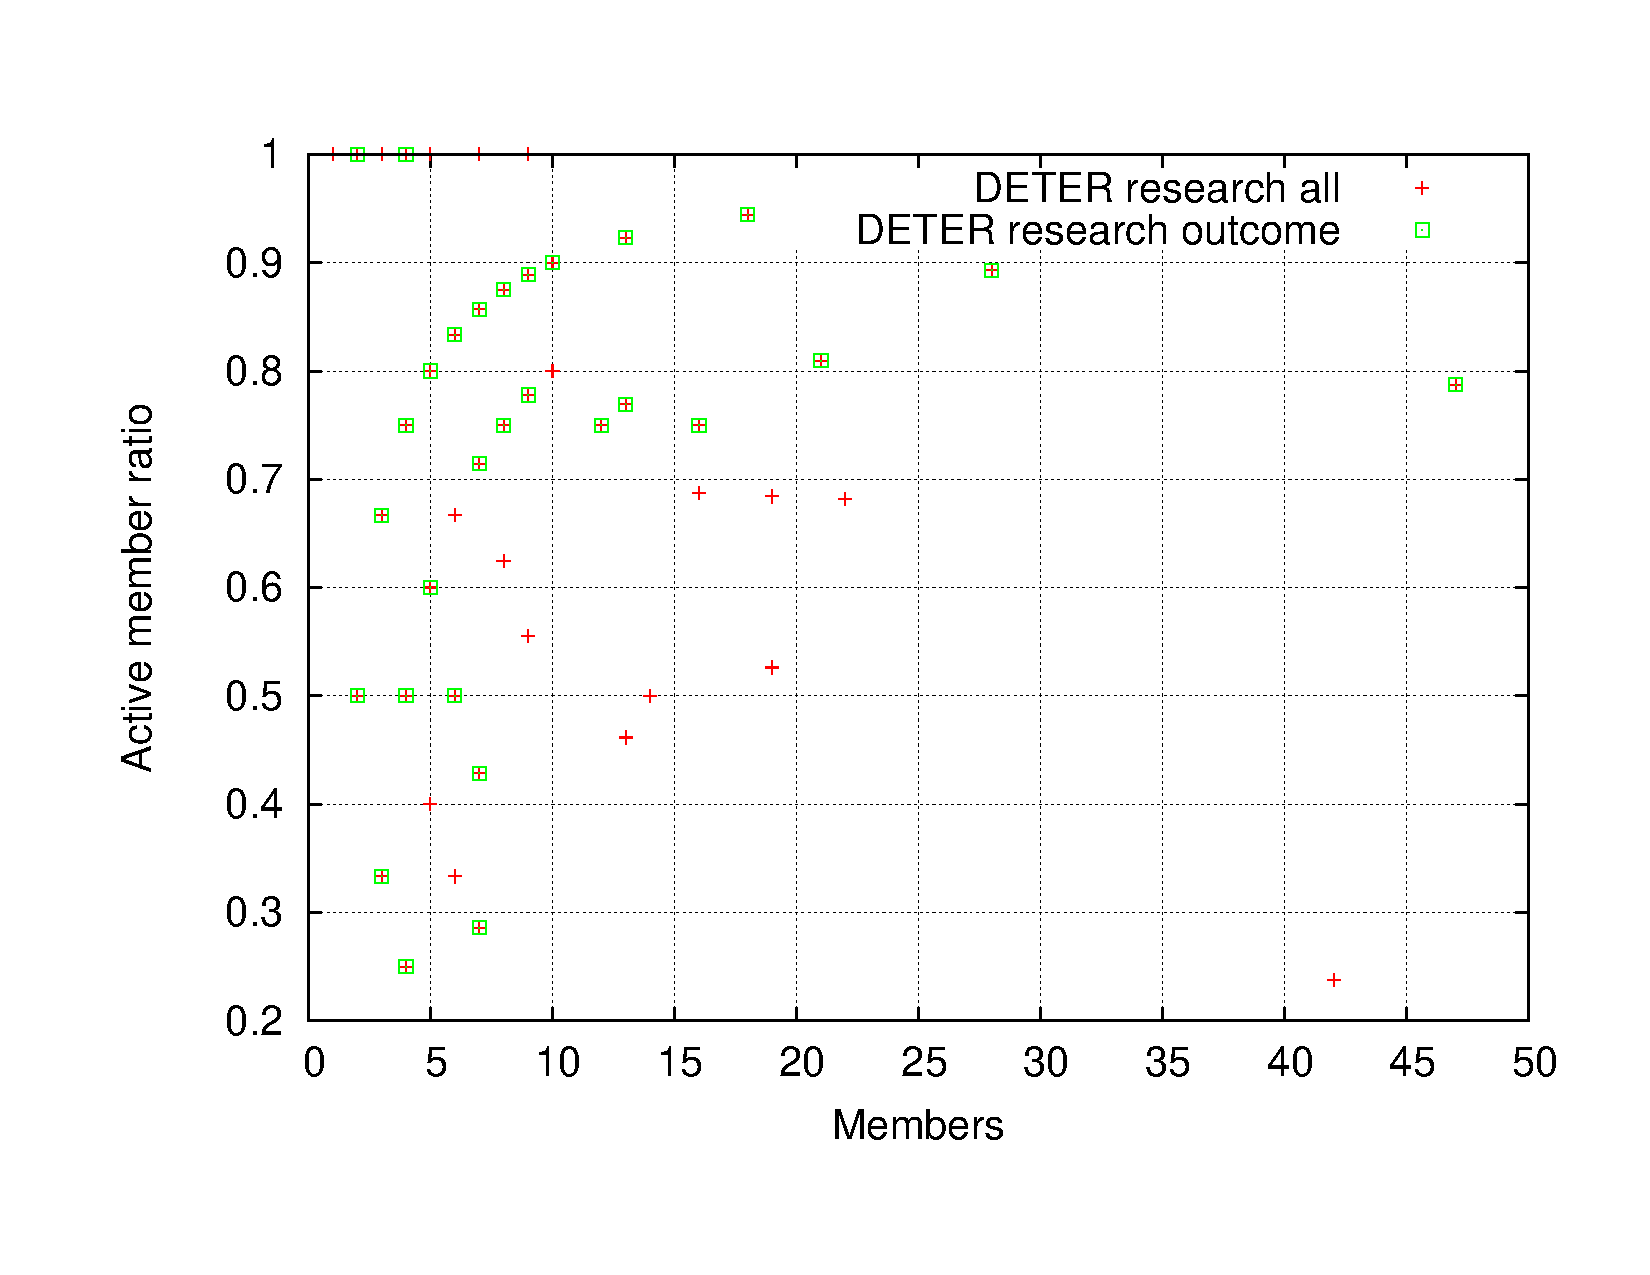
\includegraphics[width=3in,
type=pdf,ext=.pdf,read=.pdf]{figs/proj.uservsauserres.gnu}
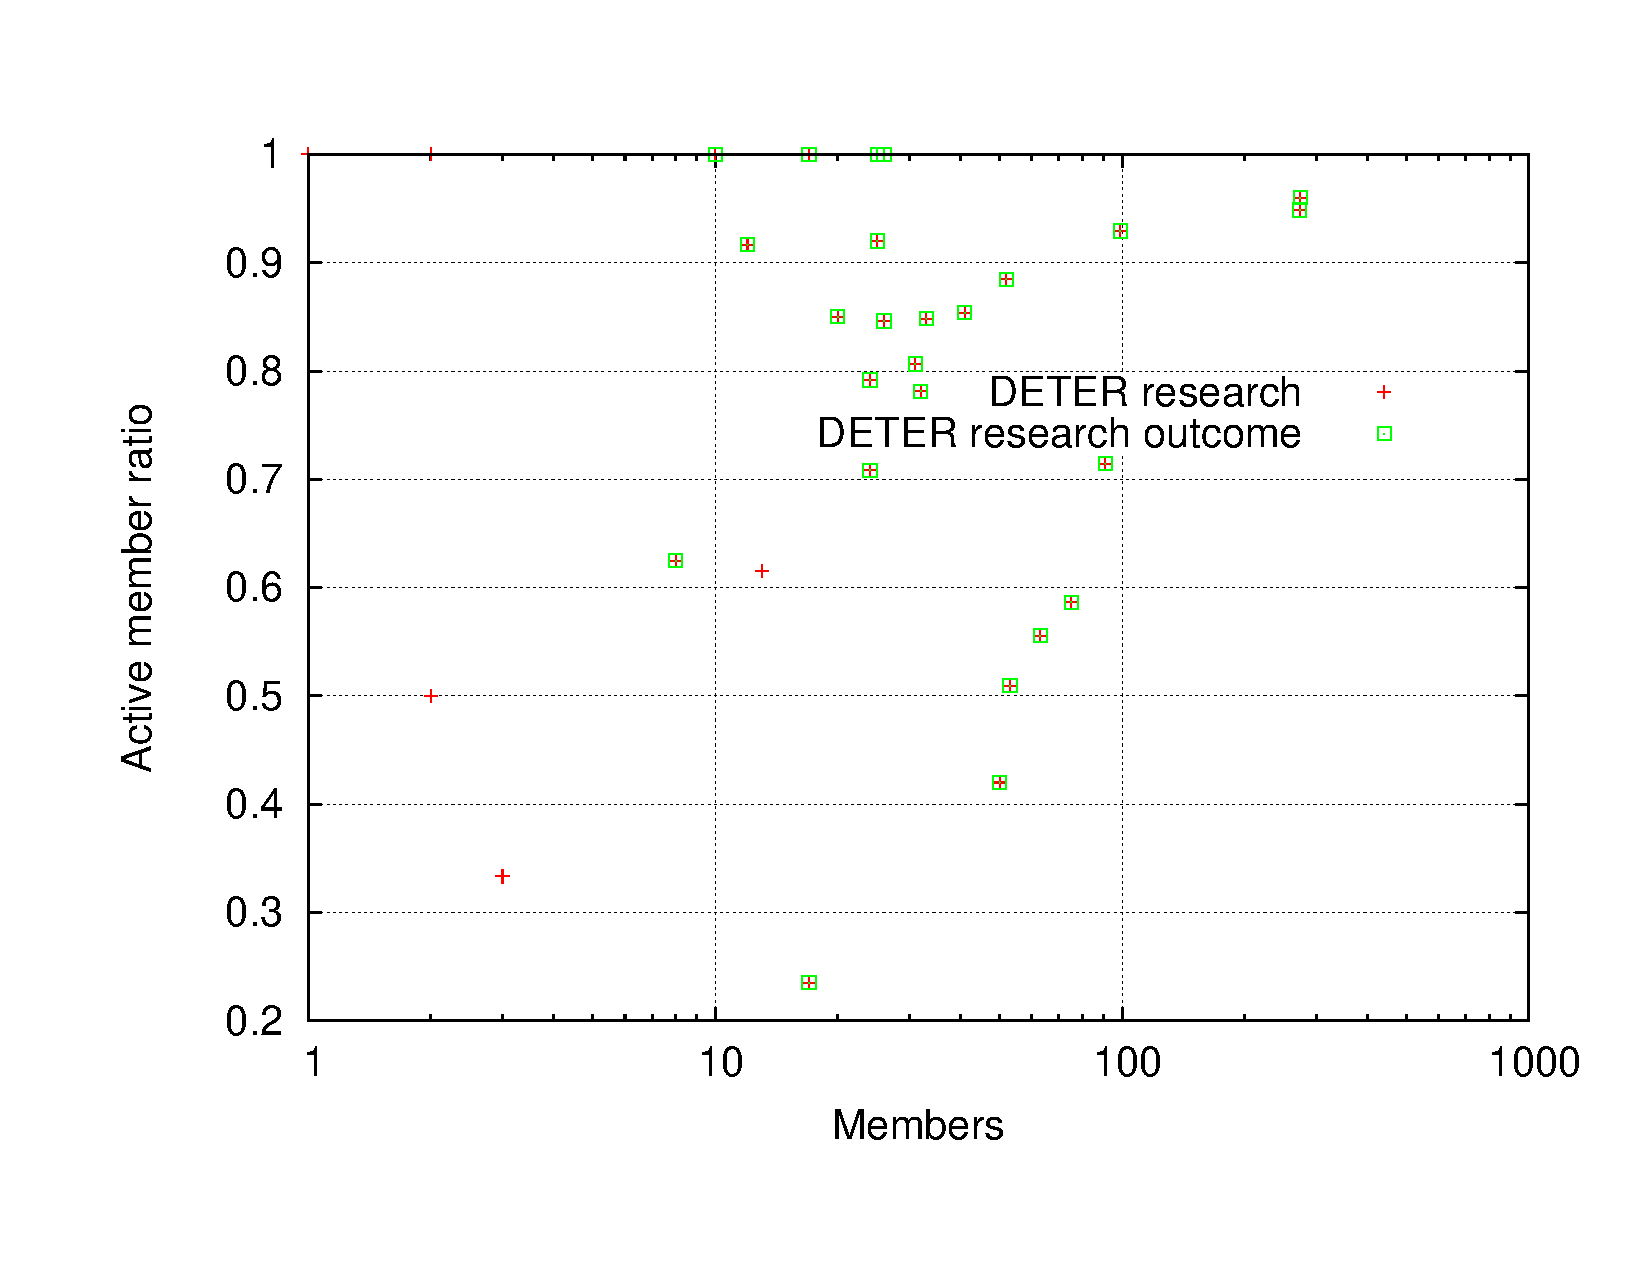
\includegraphics[width=3in,
type=pdf,ext=.pdf,read=.pdf]{figs/proj.uservsausercl.gnu}
\caption{Active member ratio vs all members of a project. Left: DETER
research, right: DETER class} \label{projuservsauser} \end{center}
\end{figure*}

Explain project evolution from inception to publication. Quantify how
many projects do not result in productive use. Some don't manipulate
experiments at all. Some are idle. Quantify this for users as well.
Quantify this for experiments and for idleness as well. Not sure if
idleness goes here.



\subsection{User Distributions} 


\begin{figure*}[htbp] \begin{center} 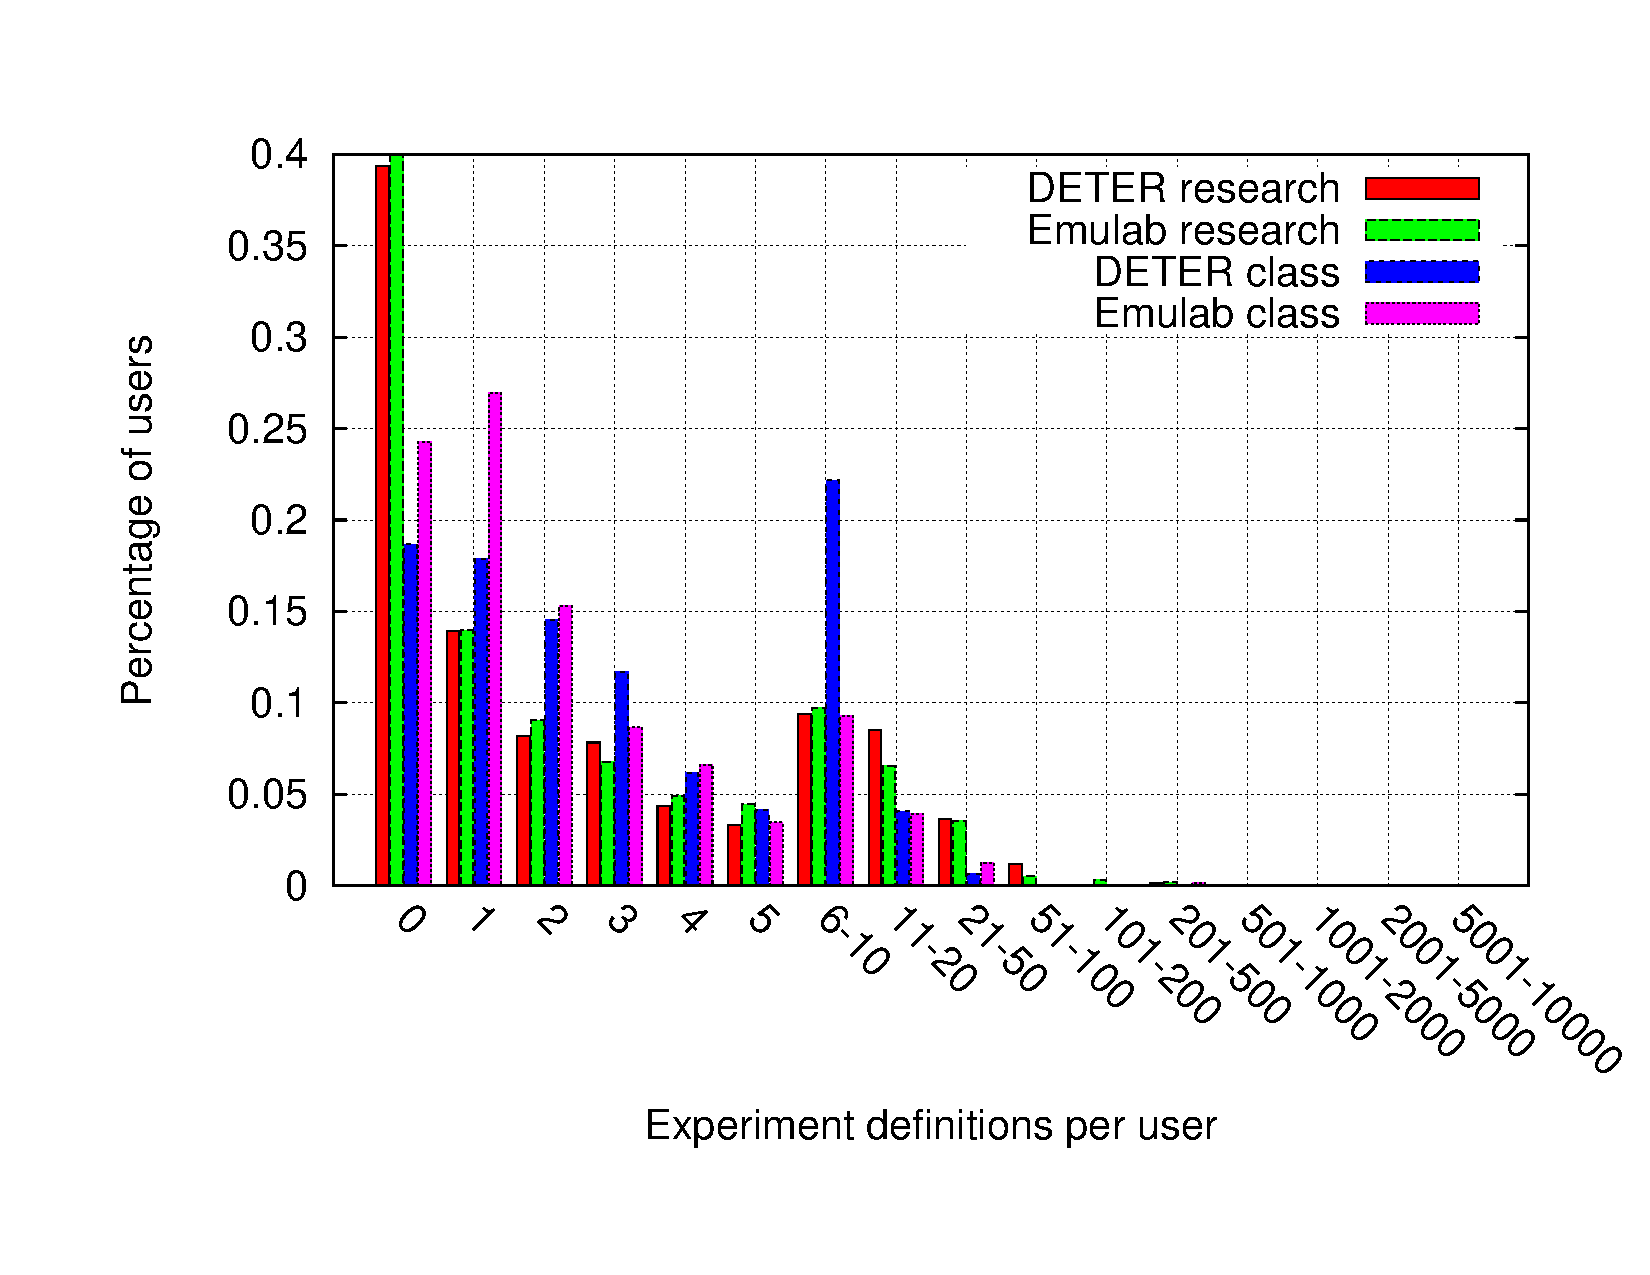
\includegraphics[width=3in,
type=pdf,ext=.pdf,read=.pdf]{figs/user.exp.gnu}
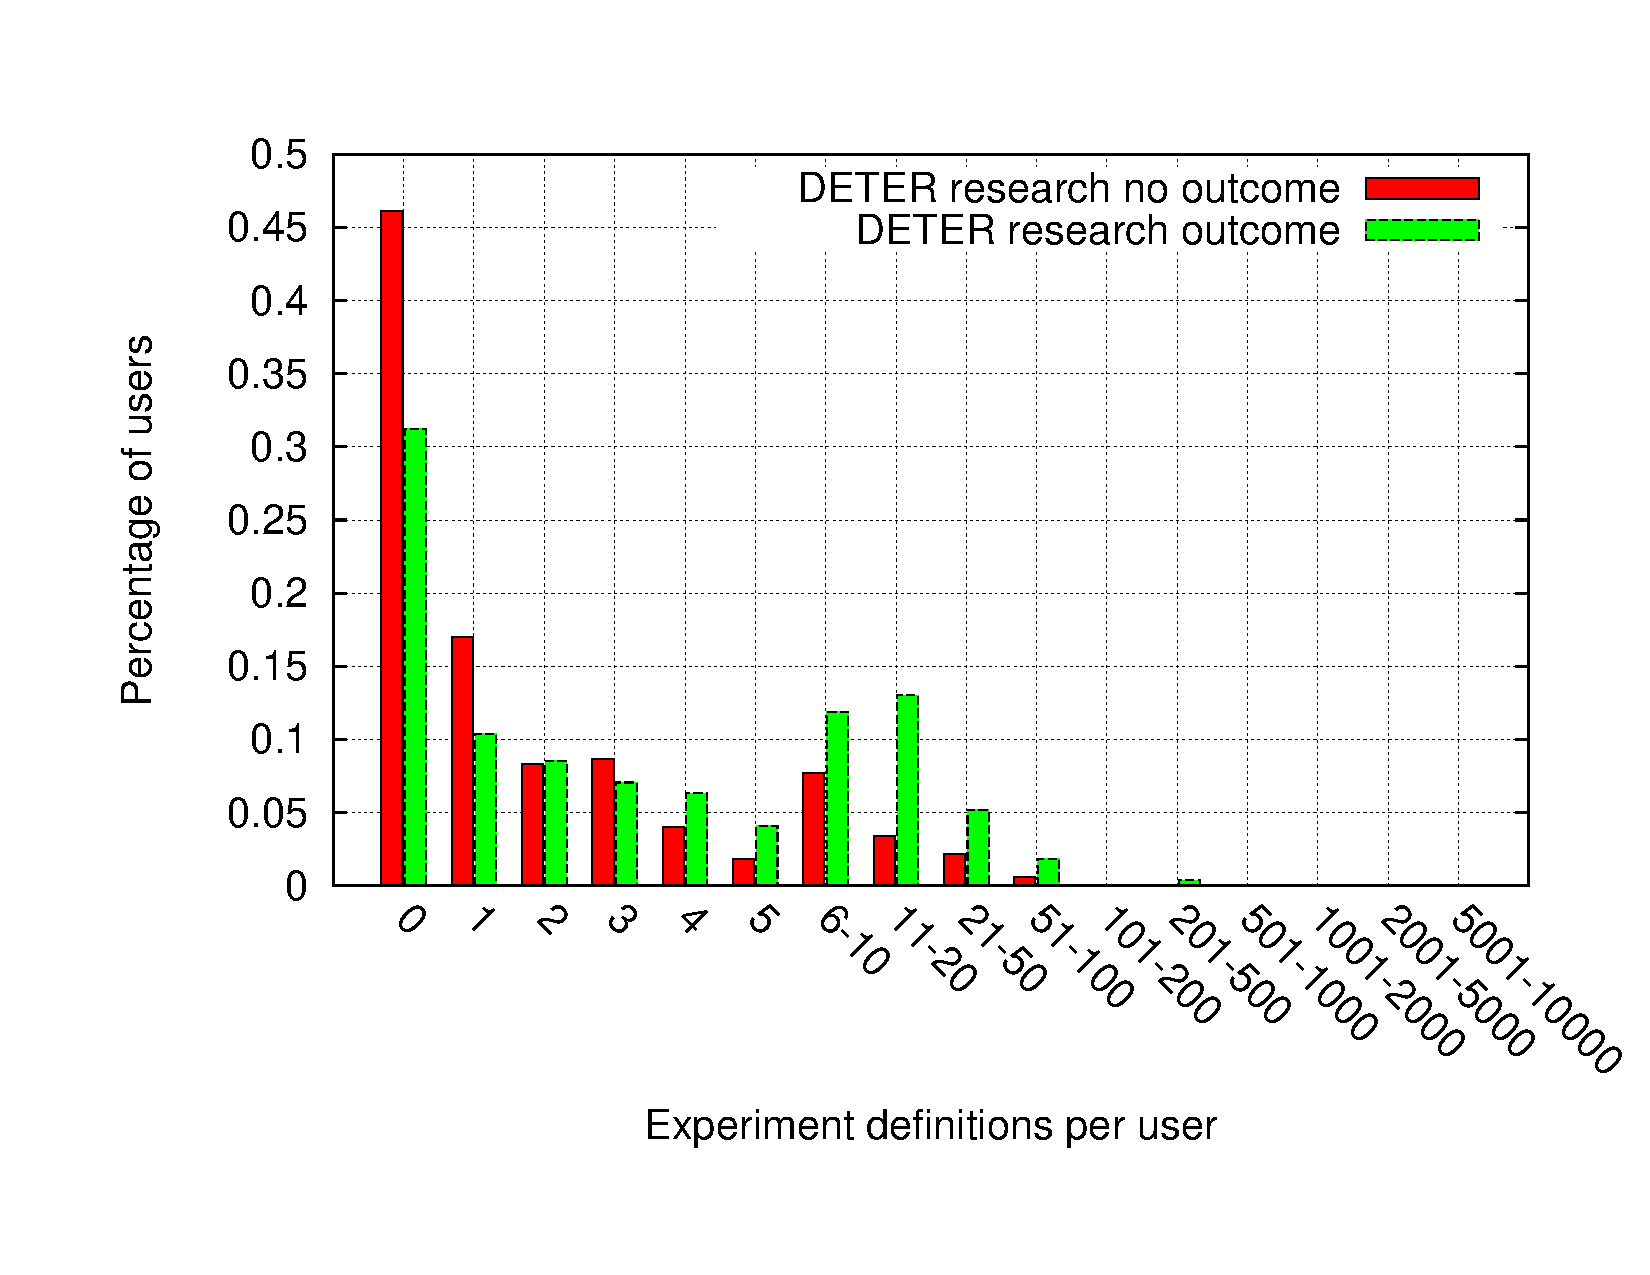
\includegraphics[width=3in,
type=pdf,ext=.pdf,read=.pdf]{figs/user.exp.cmp.gnu} 
\caption{Experiment
definitions per user. Left: DETER vs Emulab, Right: All vs outcome}
\label{userexp} \end{center} \end{figure*}

\begin{figure*}[htbp] \begin{center} 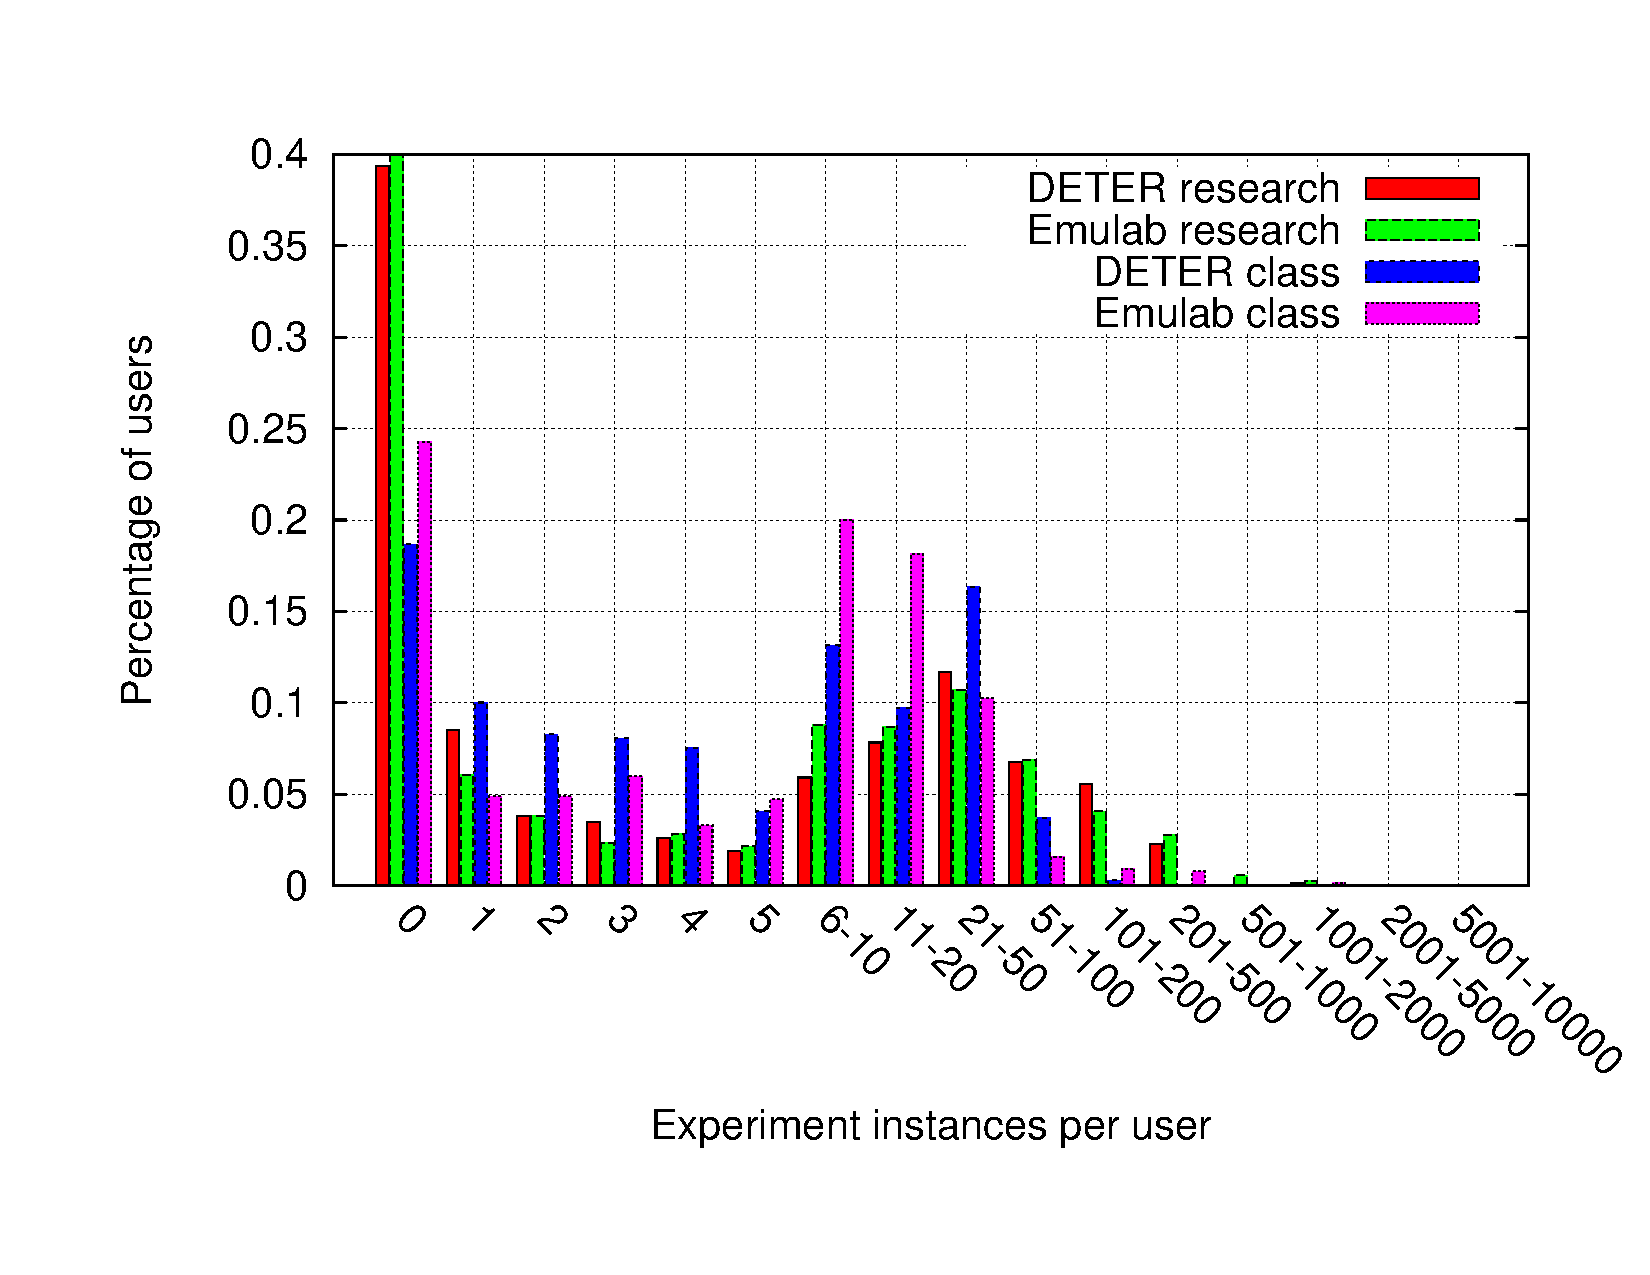
\includegraphics[width=3in,
type=pdf,ext=.pdf,read=.pdf]{figs/user.swaps.gnu}
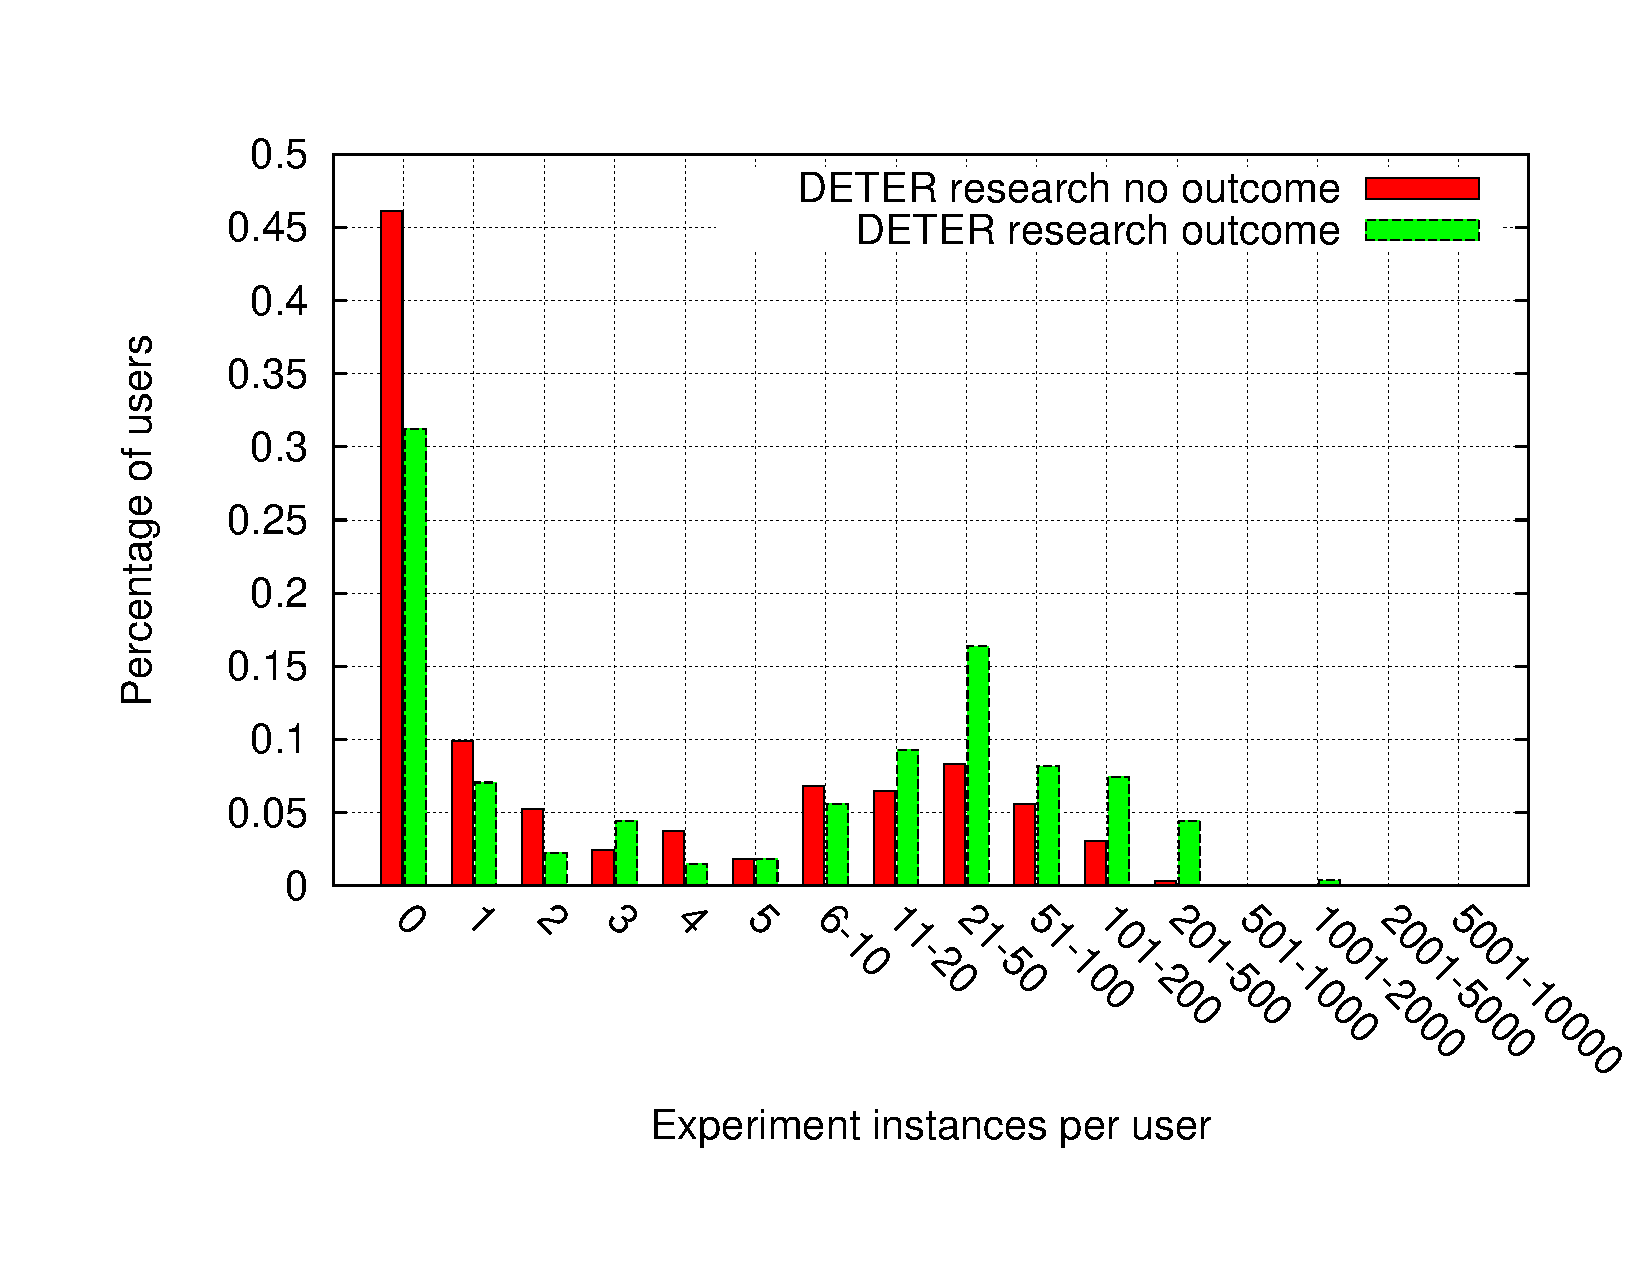
\includegraphics[width=3in,
type=pdf,ext=.pdf,read=.pdf]{figs/user.swaps.cmp.gnu}
\caption{Experiment instances per user. Left: DETER vs Emulab, Right:
All vs outcome} \label{userswaps} \end{center} \end{figure*}

\begin{figure*}[htbp] \begin{center} 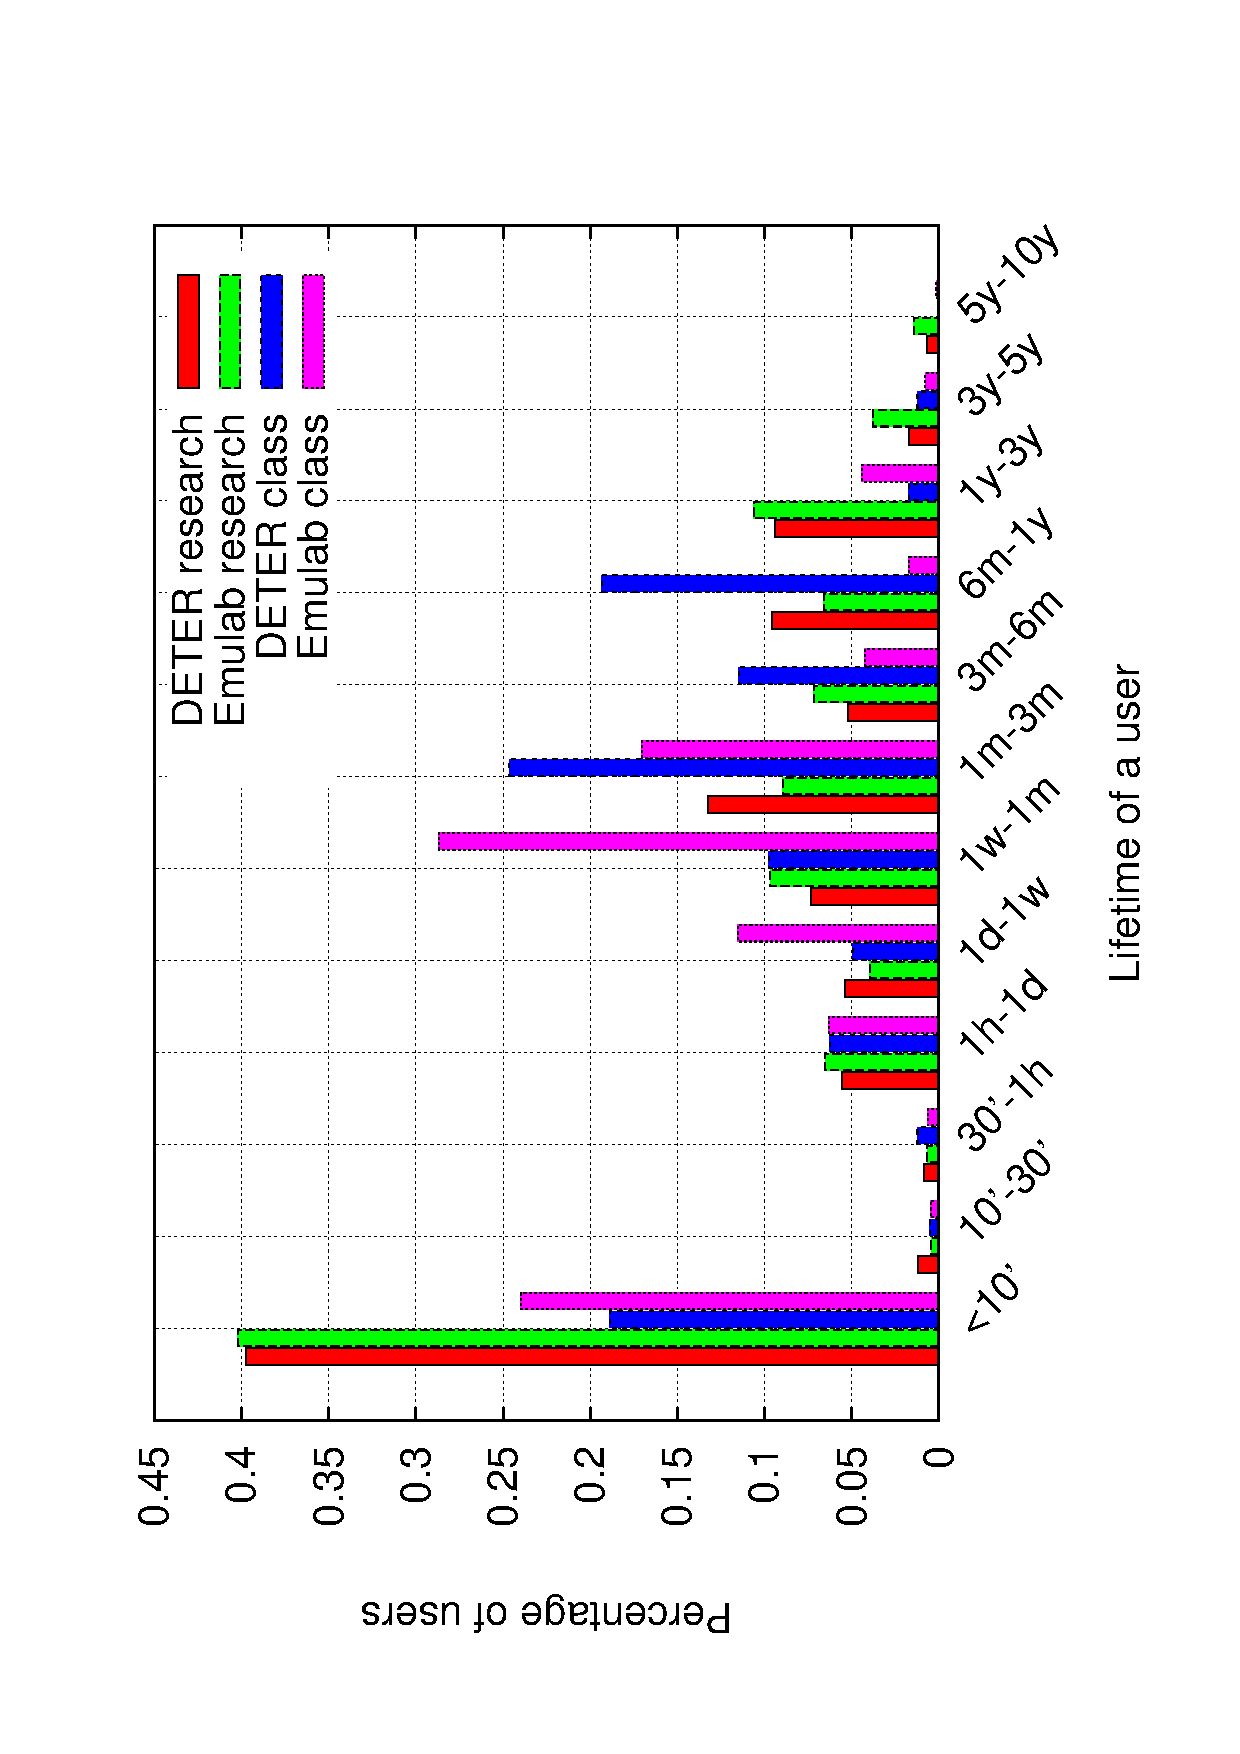
\includegraphics[width=3in,
type=pdf,ext=.pdf,read=.pdf]{figs/user.life.gnu}
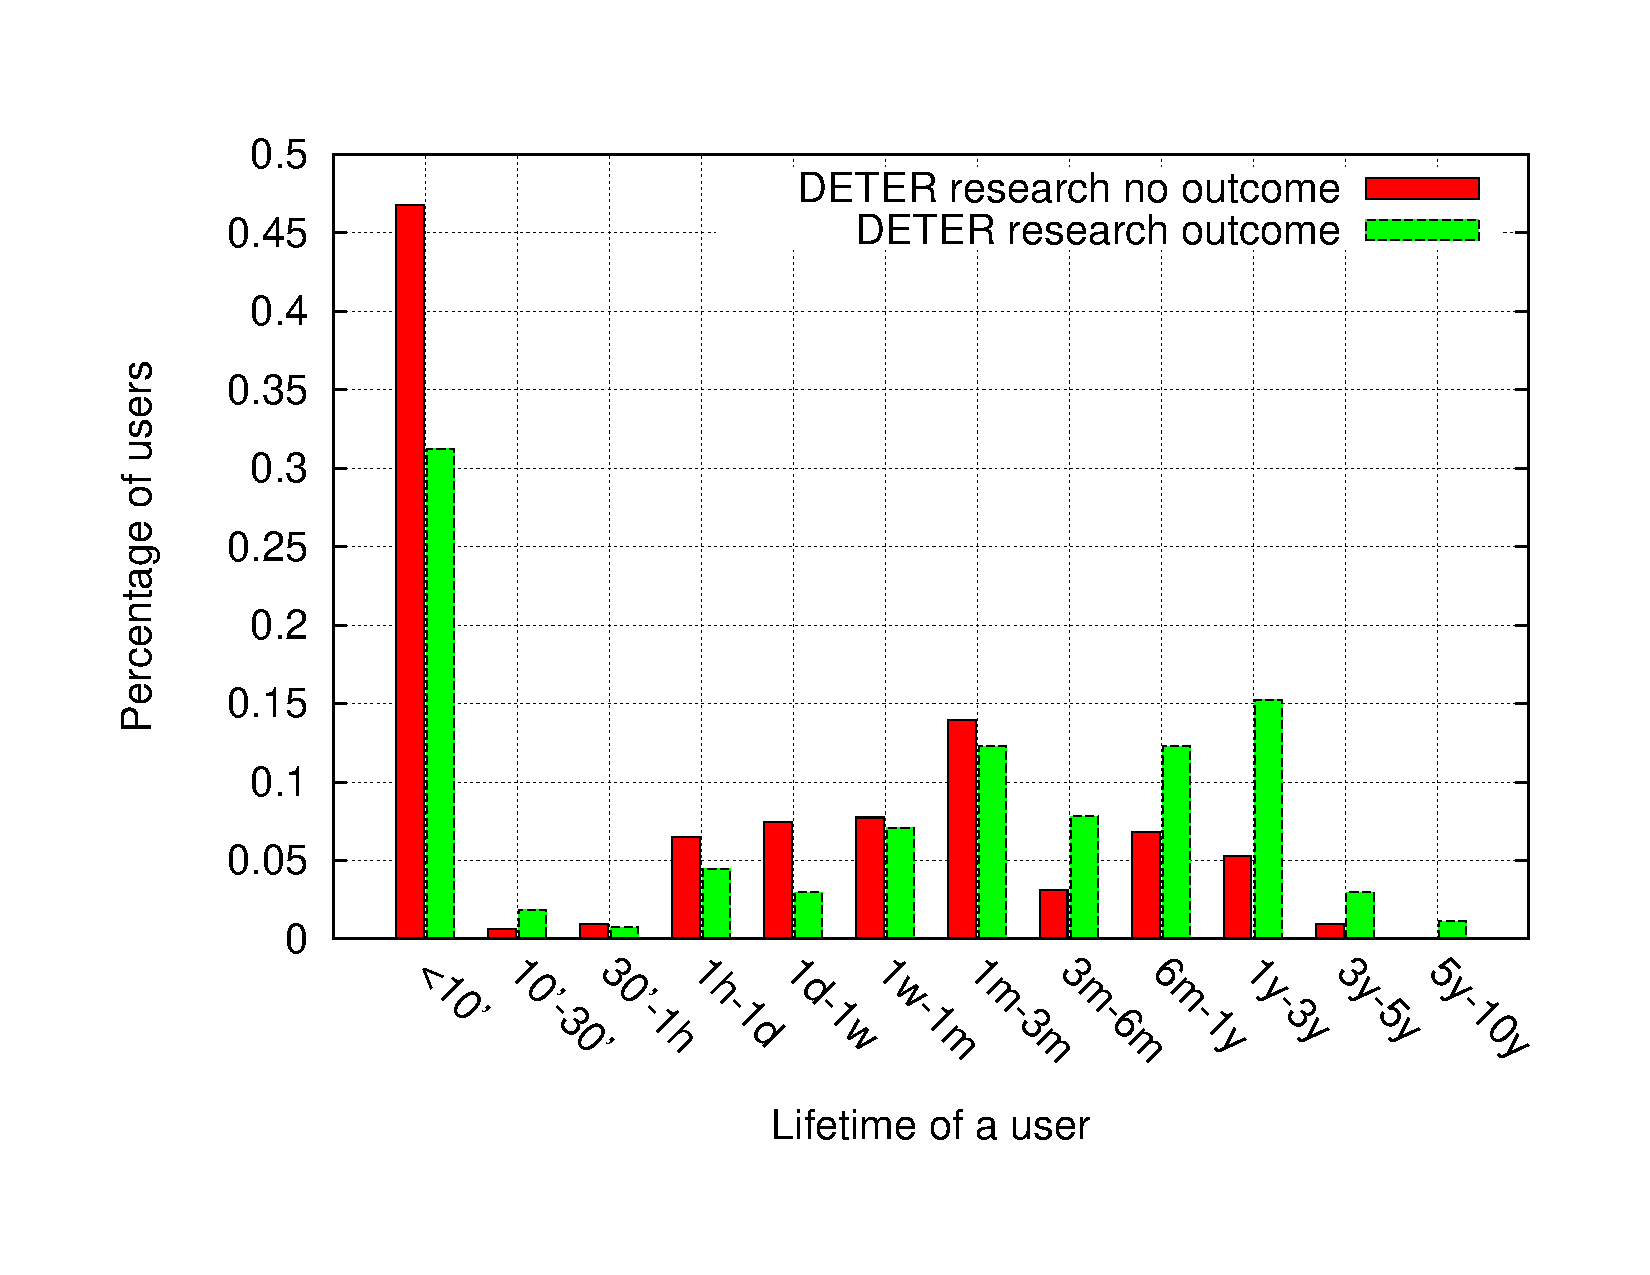
\includegraphics[width=3in,
type=pdf,ext=.pdf,read=.pdf]{figs/user.life.cmp.gnu} \caption{User
lifetime. Left: DETER vs Emulab, Right: All vs outcome} \label{userlife}
\end{center} \end{figure*}


\begin{figure*}[htbp] \begin{center} 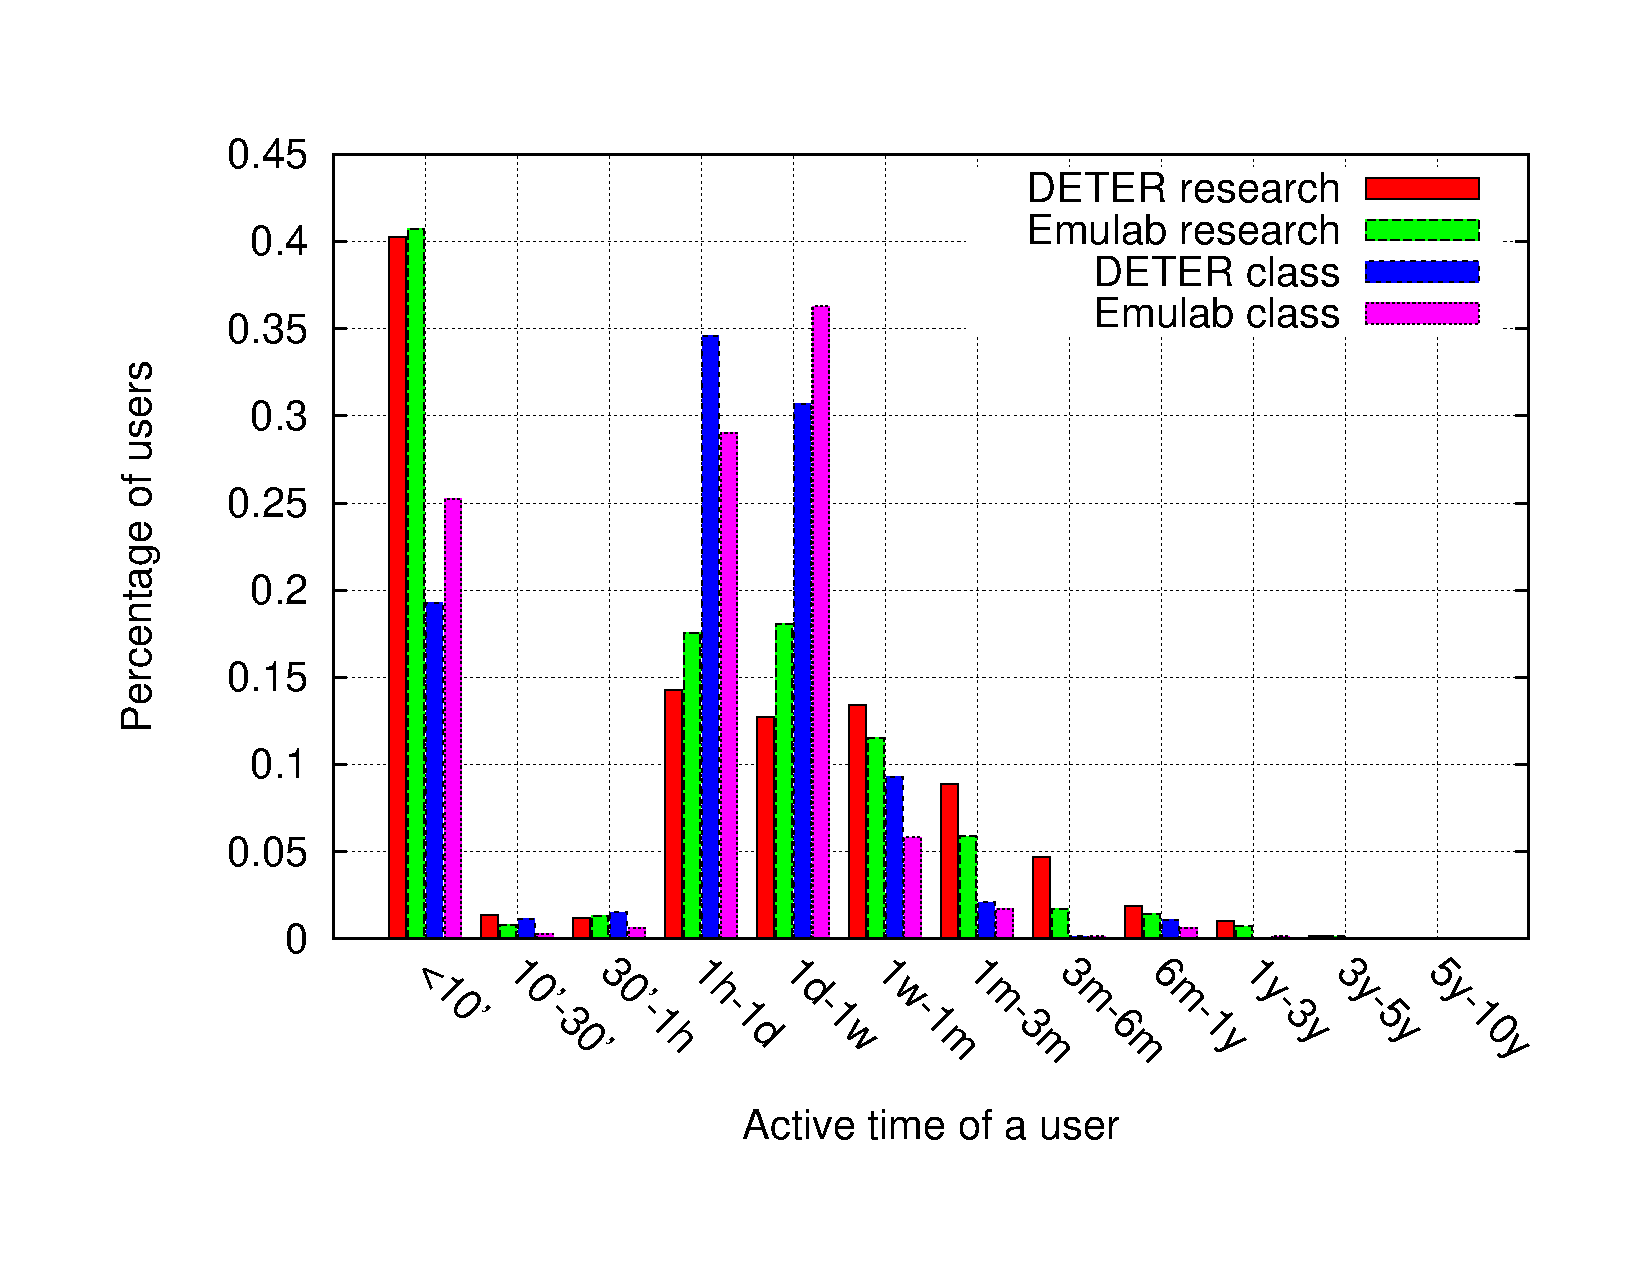
\includegraphics[width=3in,
type=pdf,ext=.pdf,read=.pdf]{figs/user.active.gnu}
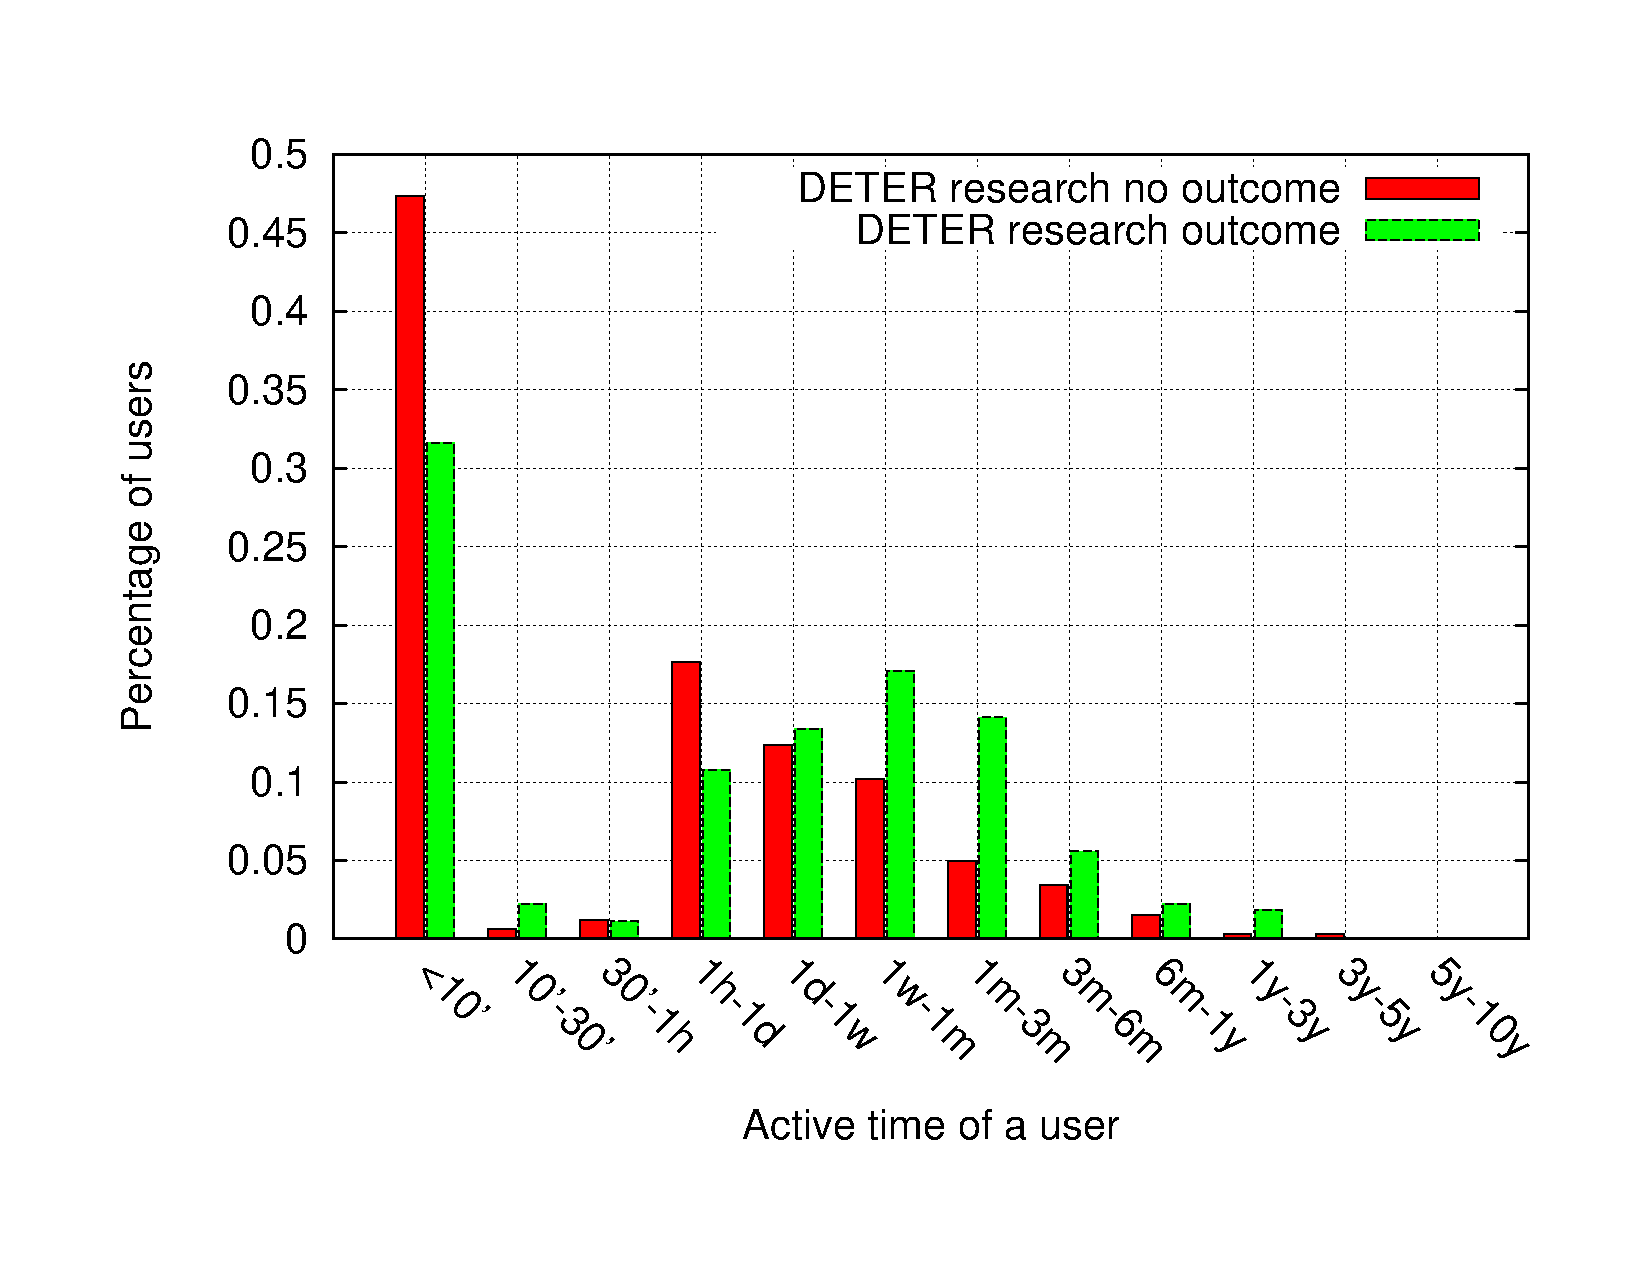
\includegraphics[width=3in,
type=pdf,ext=.pdf,read=.pdf]{figs/user.active.cmp.gnu} \caption{User
active time. Left: DETER vs Emulab, Right: All vs outcome}
\label{useractive} \end{center} \end{figure*}

\begin{figure*}[htbp] \begin{center} 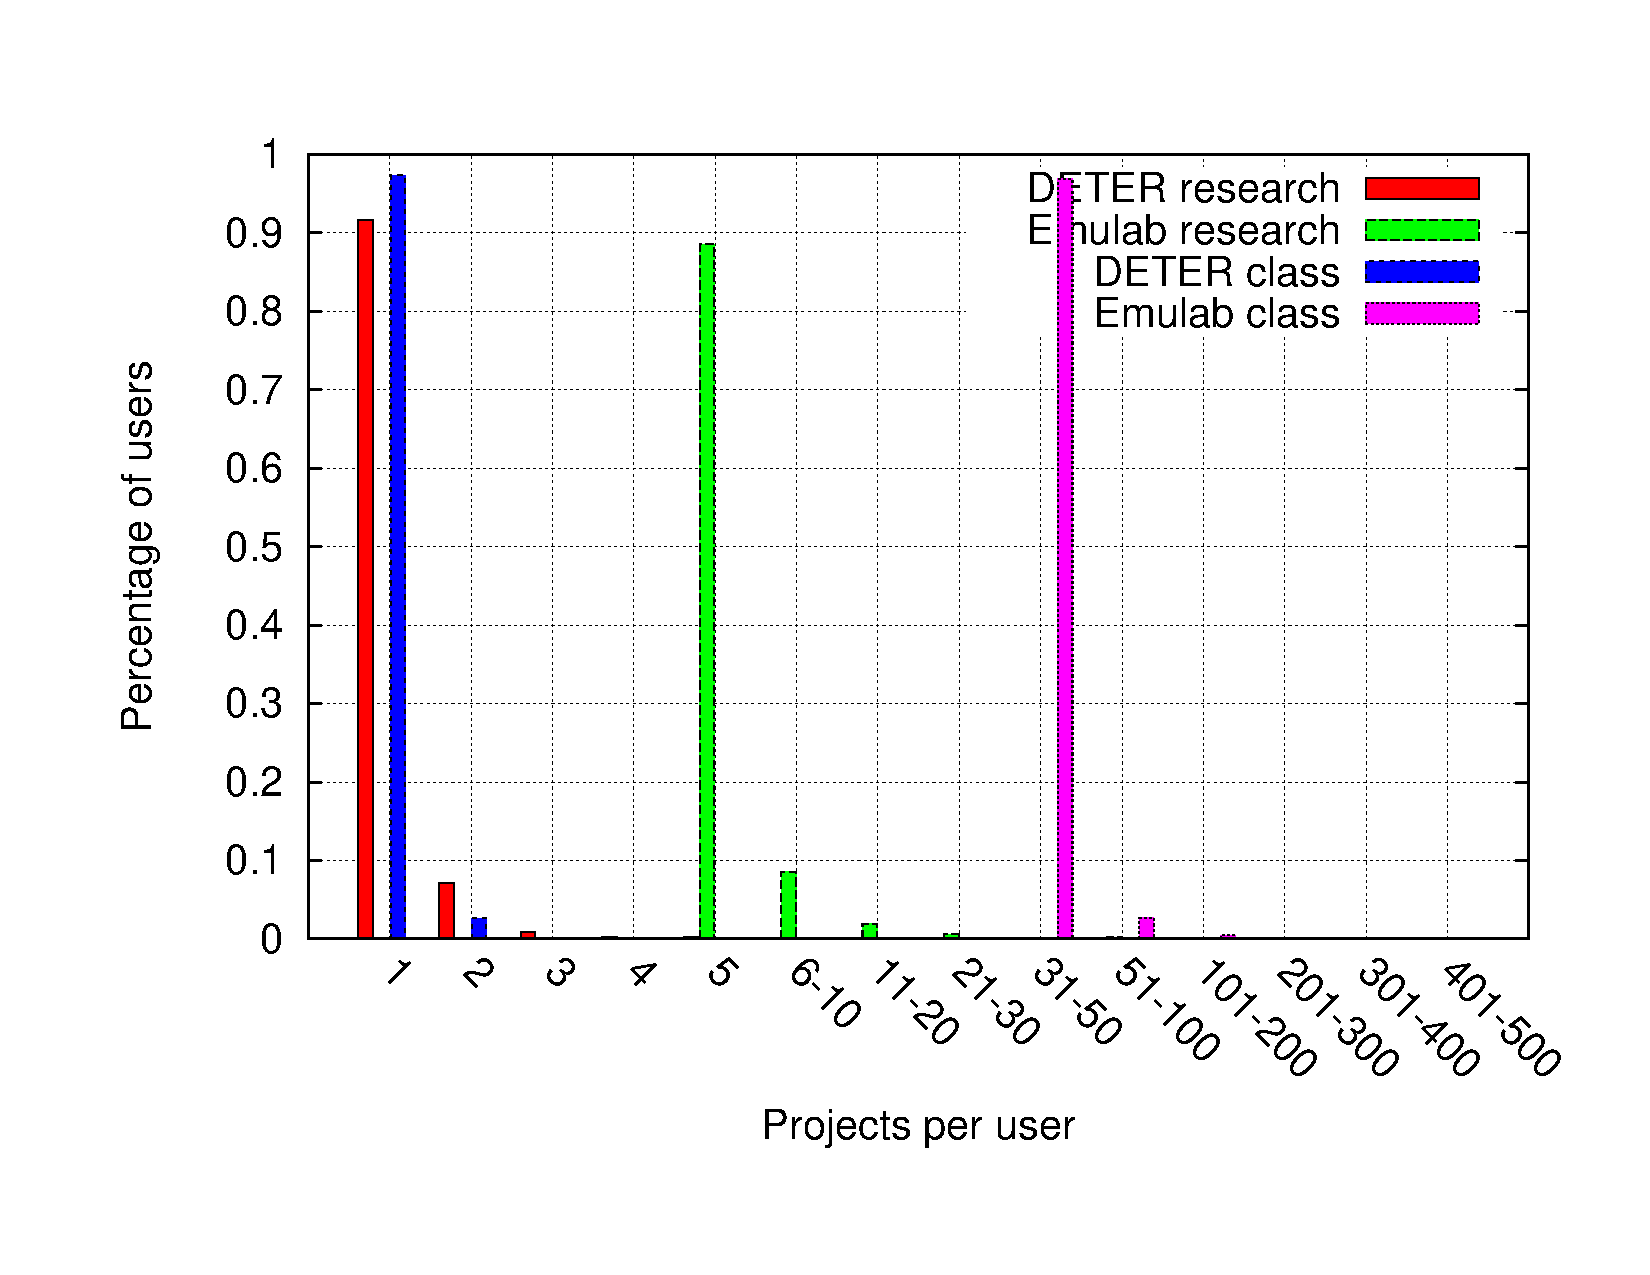
\includegraphics[width=3in,
type=pdf,ext=.pdf,read=.pdf]{figs/user.proj.gnu}
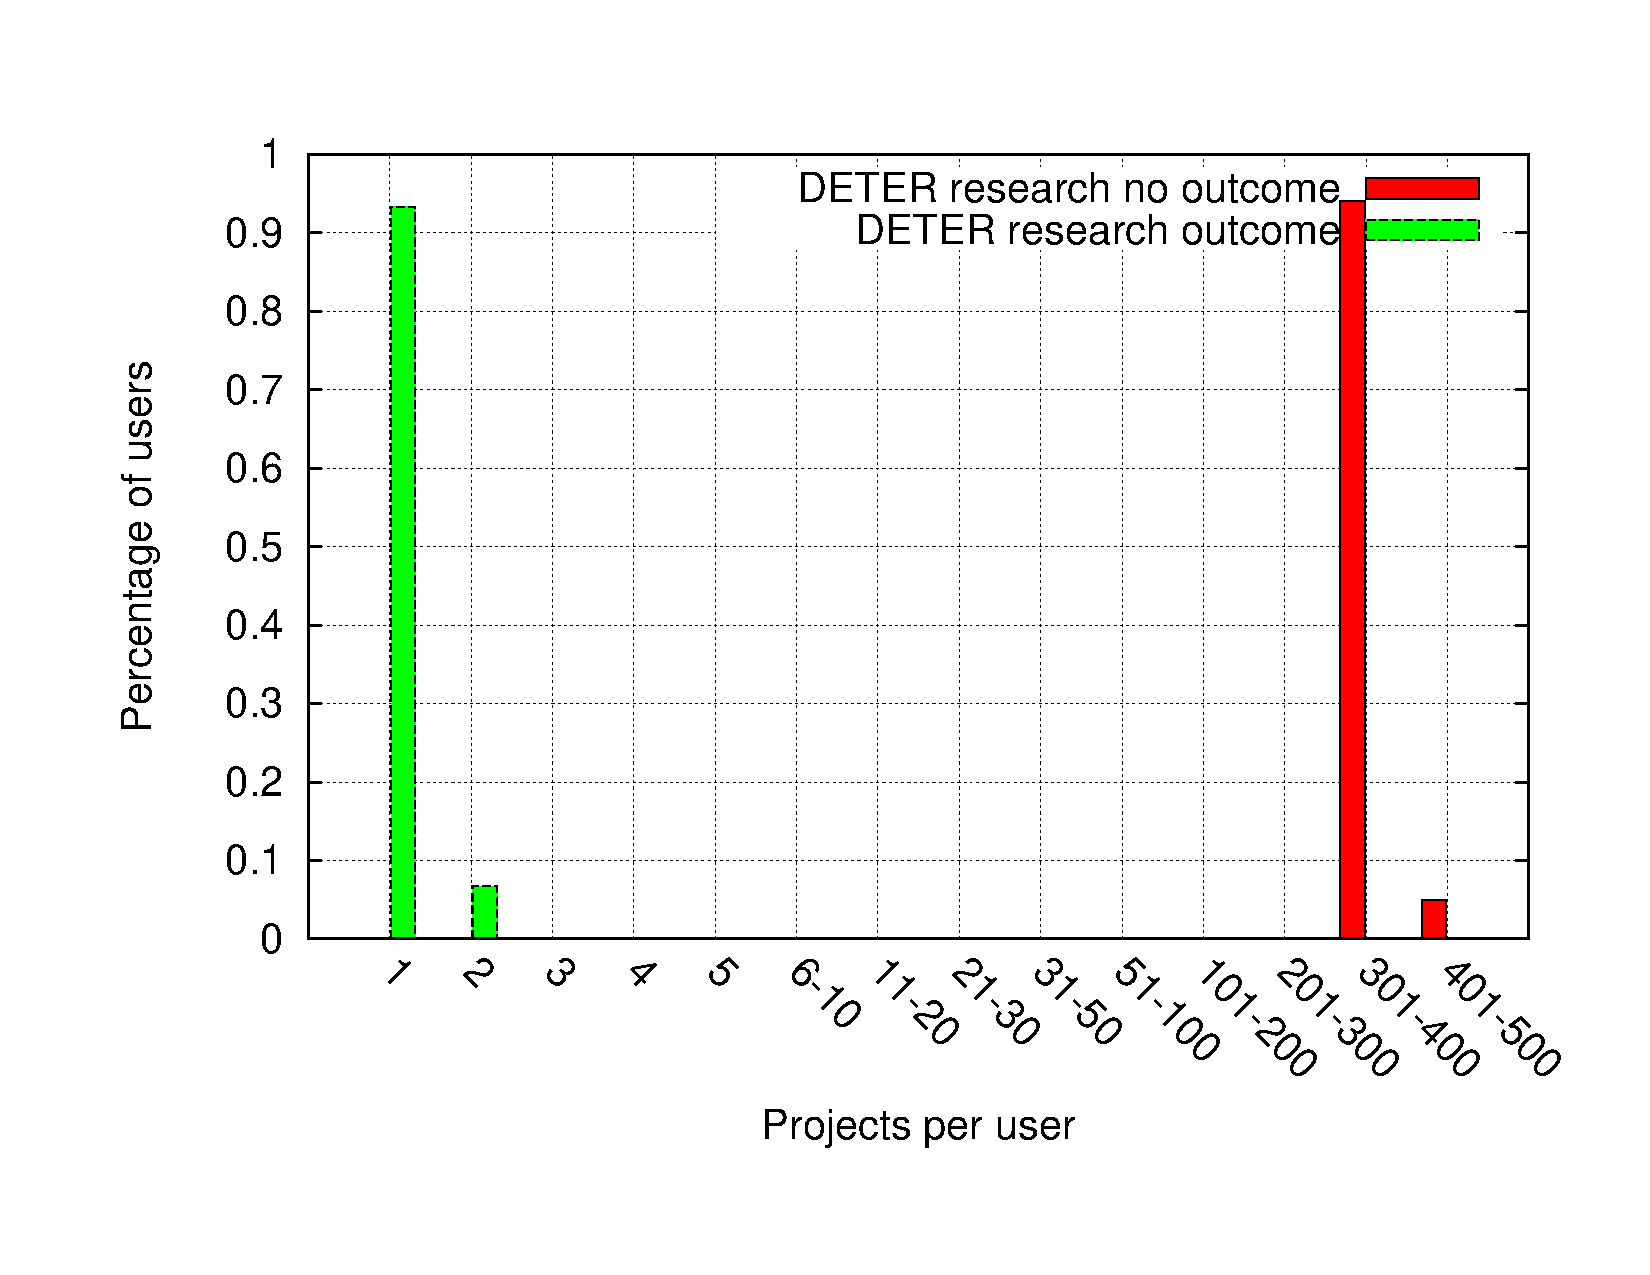
\includegraphics[width=3in,
type=pdf,ext=.pdf,read=.pdf]{figs/user.proj.cmp.gnu} \caption{Projects
per user. Left: DETER vs Emulab, Right: All vs outcome} \label{userproj}
\end{center} \end{figure*}

Members can be deleted and we don't account for that



\subsection{Geolocation Distribution} 



\begin{table}[htdp] \caption{Node activity} \begin{center}
\begin{tabular}{|c|c|} \hline Activity & Percentage \\ \hline Idle &
57\% \\ Network & 30\% \\ CPU & 10\\ Interactive & 3 \\ \hline
\end{tabular} \end{center} \label{default} \end{table}%

57\% of timeslots reported by allocated node were idle but per
experiment all nodes are used together. There are really no huge
inactive periods so inactivity is spread through the experiment. 26\% of
timeslots report a network activity. 6.8\% report a CPU activity and 2\%
report a CPU and network activity.

\begin{figure*}[htbp] \begin{center} 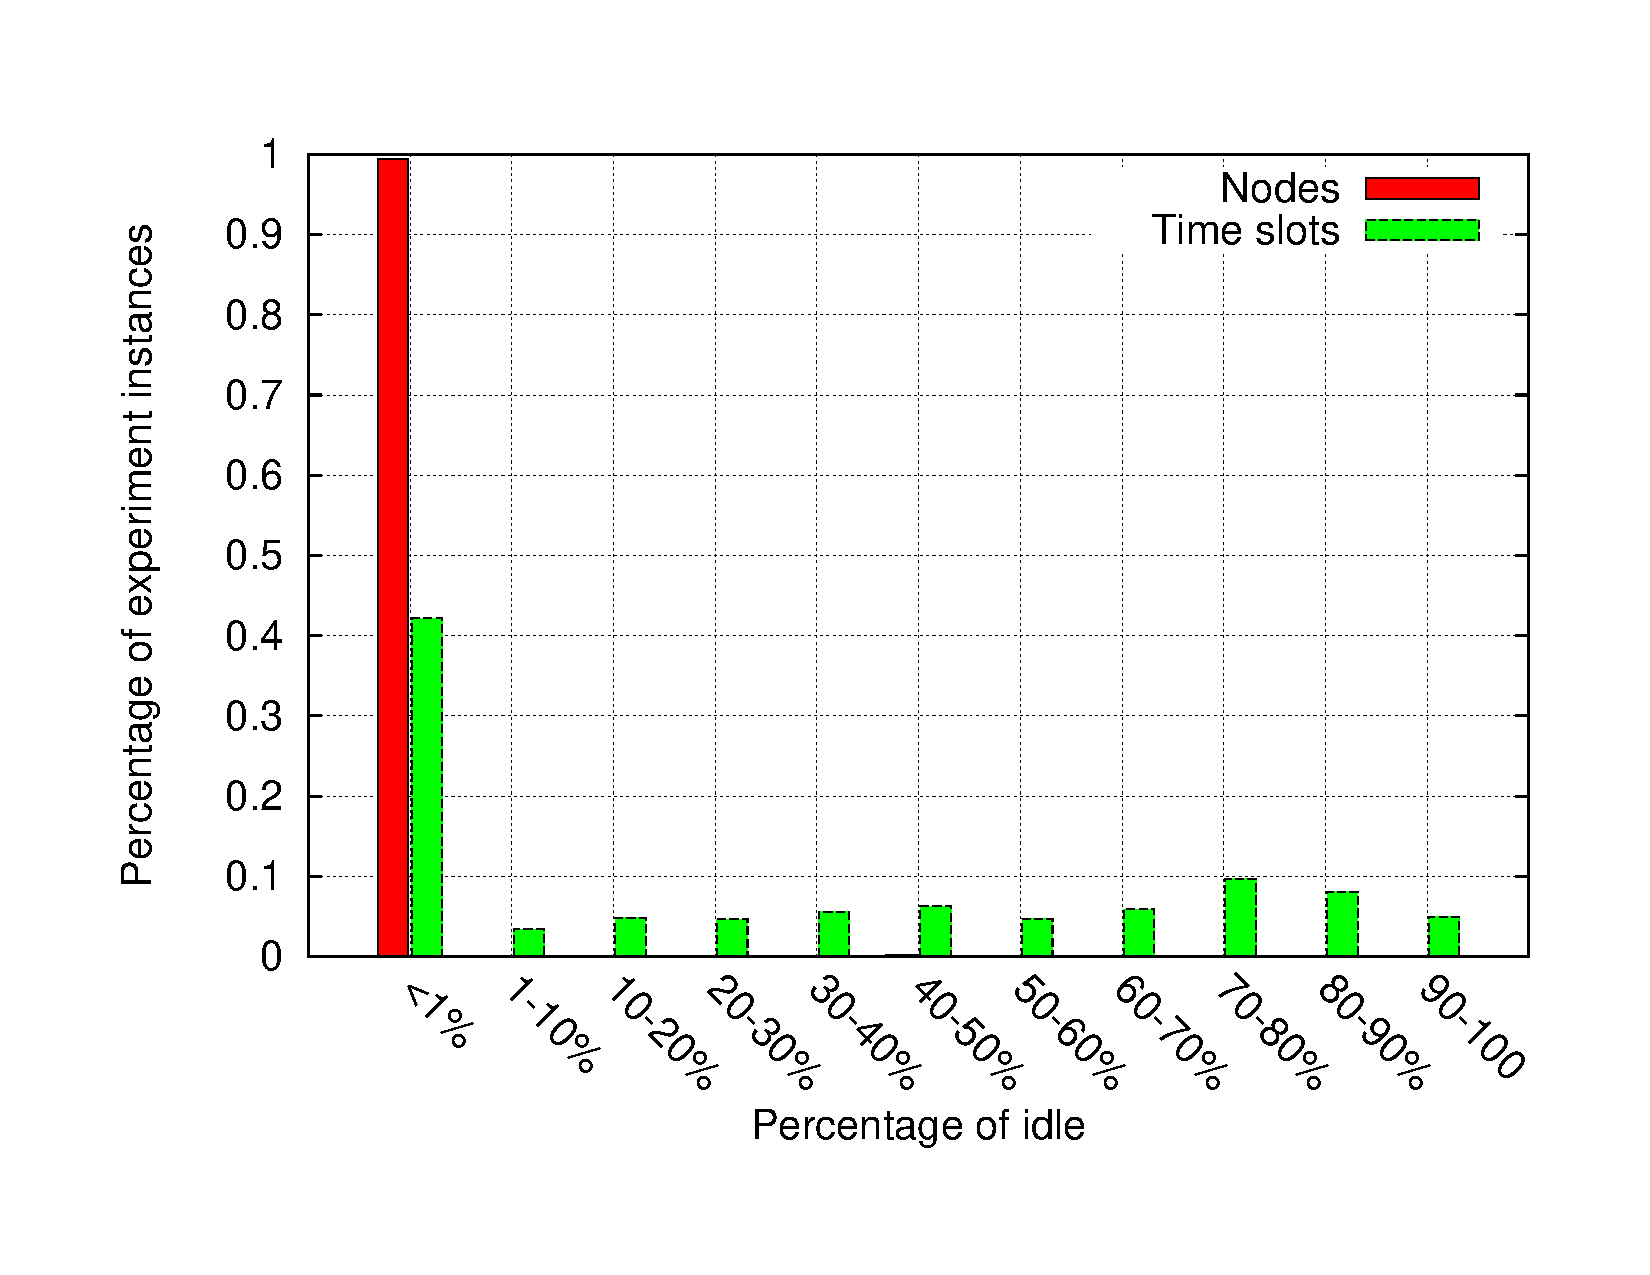
\includegraphics[width=3in,
type=pdf,ext=.pdf,read=.pdf]{figs/exp.idle.gnu}
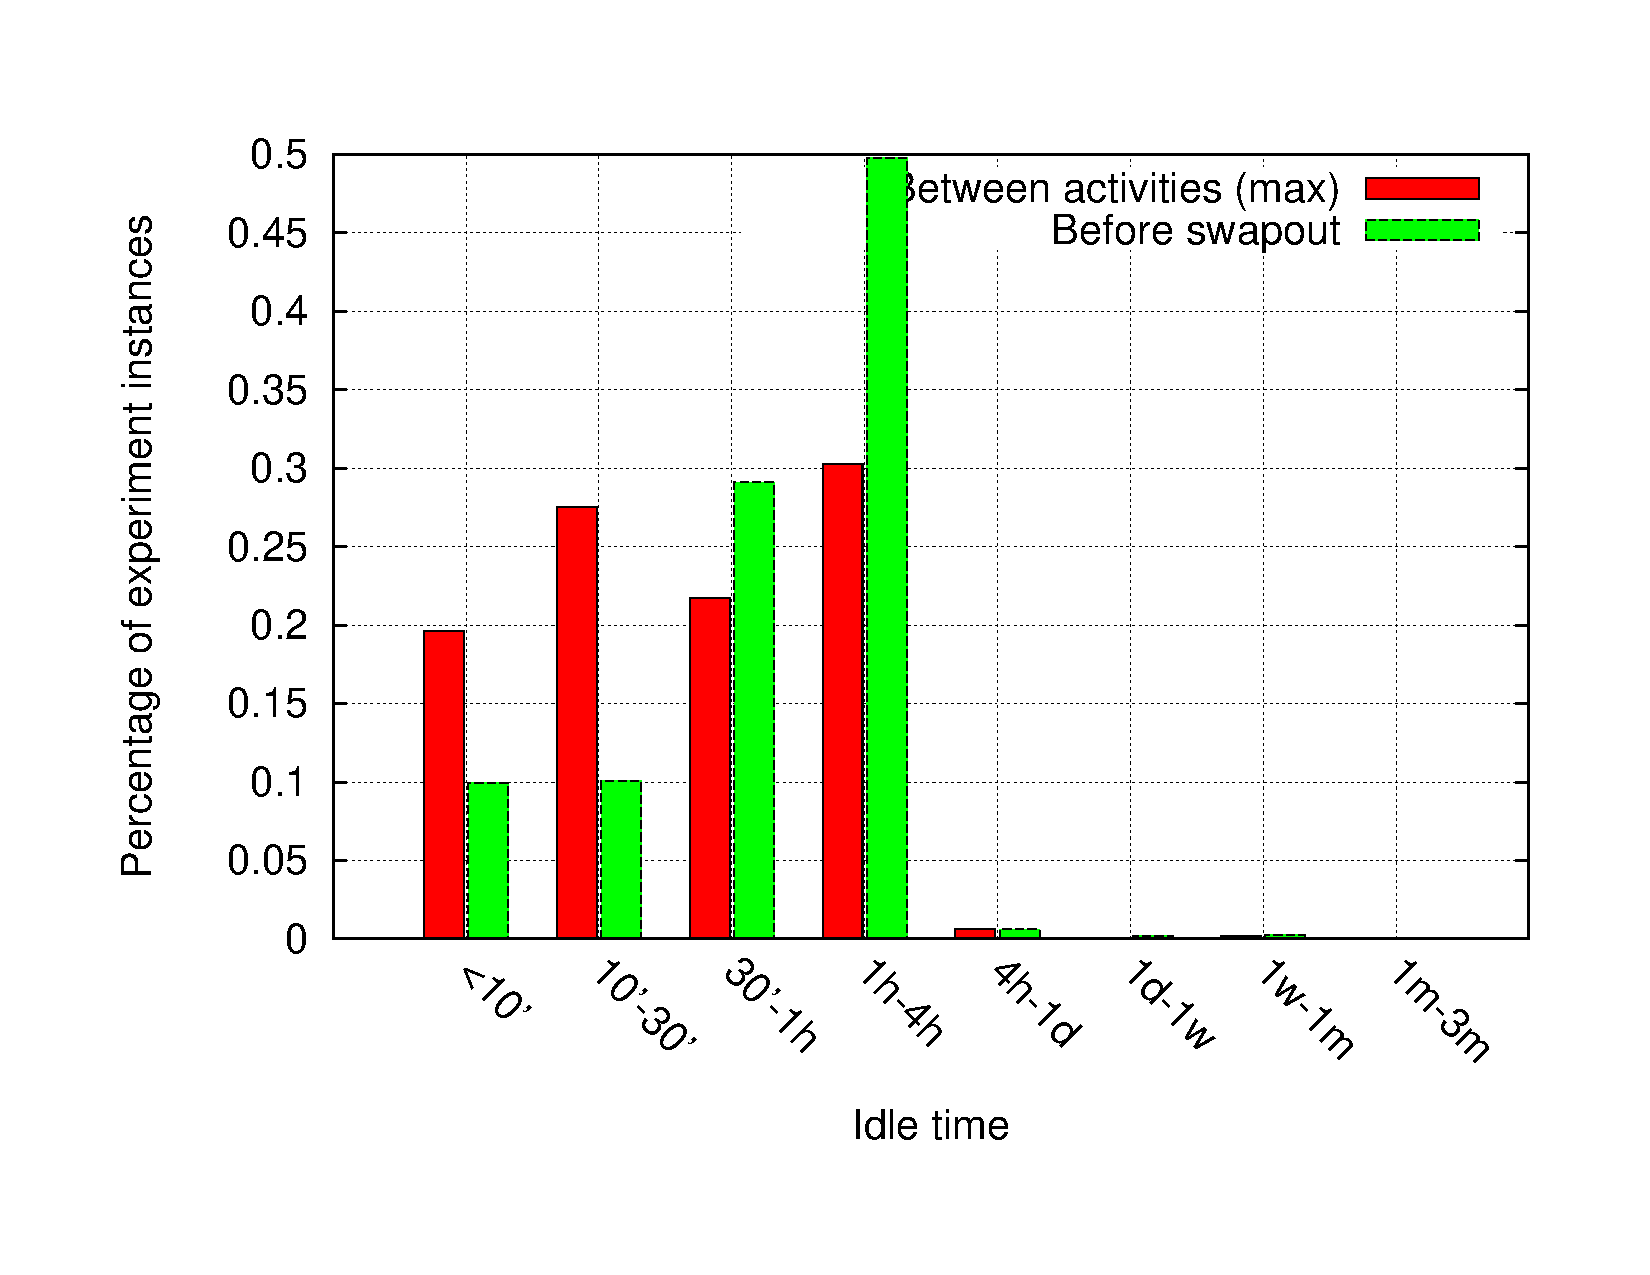
\includegraphics[width=3in,
type=pdf,ext=.pdf,read=.pdf]{figs/period.idle.gnu} \caption{Idleness per
experiment} \label{idle} \end{center} \end{figure*}


cummulative per project idle nodes correlate with experiment duration?
correlate with experiment history?


